\documentclass[12pt]{report}
\usepackage{mystyle}
\setlength{\abovedisplayskip}{2pt}
\setlength{\belowdisplayskip}{2pt}
\usepackage{nccmath}
\usepackage{xpatch}
\xpatchcmd{\NCC@ignorepar}{%
\abovedisplayskip\abovedisplayshortskip}
{%
\abovedisplayskip\abovedisplayshortskip%
\belowdisplayskip\belowdisplayshortskip}
{}{}
\usetikzlibrary{positioning, arrows.meta}
\tikzset{%
    myarrow/.style = {-Stealth, shorten >=3pt}
} 
\newcommand{\mypoint}[2]{\tikz[remember picture]{\node[inner sep=0, anchor=base](#1){$#2$};}}
\usepackage{arydshln}
\makeatletter
\newcommand*\dashline{\rotatebox[origin=c]{90}{$\dabar@\dabar@\dabar@$}}
\makeatother
\begin{document}
% \righthyphenmin=2
\chapter{Алгебра и геометрия. \\ \hfill Линейная алгебра}

\begin{multicols}{2}
\raggedcolumns 

\section{Группы, кольца, поля. Определения и примеры. Циклические группы. Теорема о гомоморфизме}

\begin{definition}{(Группа)}{}
    Непустое множество $\mathcal{G}$, на котором определена некая операция $\bullet: \mathcal{G} \times \mathcal{G} \to \mathcal{G}$, называется группой, если выполнены 3 свойства: $(\forall a,b,c \in \mathcal{G})$
    \begin{enumerate*}
        \item ассоциативность $a\bullet(b\bullet c) = (a\bullet b)\bullet c$;
        \item существование нейтрального элемента $\exists e \in \mathcal{G}: e\bullet a = a\bullet e = a$;
        \item существование обратного элемента $\exists a^{-1}\in \mathcal{G} : a\bullet a^{-1} = a^{-1}\bullet a = e\in \mathcal{G}$;
    \end{enumerate*}  
\end{definition}
Если $(\mathcal{G}, \bullet)$ удовлетворяет только свойству 1., то множество называется полугруппой. Если свойства 1. и 2., то моноид.
Пример: 
\begin{multicols}{2}
    \begin{enumerate*}
    \item $\left(\Z, +\right)$ -- группа;
    \item $\left(\Z, \cdot\right)$ -- моноид;
    \item $\left(\Q\backslash \left\{0\right\}\right)$ -- группа;
    \item $\left(\R, +\right)$ -- группа;
    \item $\left(\R \backslash \{0\}\right)$ -- группа.
\end{enumerate*}
\end{multicols}
\begin{note}
    Абелевой группой называется группа $(\mathcal{G}, \bullet)$ в соответствии с определением, но обладающая также коммутативностью: \[\forall a,b \in \mathcal{G} \ ab = ba\]
\end{note}
Примеры:
\begin{multicols}{2}
\begin{enumerate*}
    \item $(V_{2,3})$ -- группа;
    \item $(M_{n\times k}, +)$ -- группа;
    \item $(M_{n\times n}, \cdot)$ -- моноид;
    \item $S_n = \{\sigma: \{1, \ldots, n\} \to \\ \to \{1, \ldots, n\}\}$ -- симметричная группа, но не абелева. Группа перестановок. Операция -- композиция. 
\end{enumerate*}
\end{multicols}
\begin{definition}{(Кольцо)}{}
    Множество $R$ с двумя бинарными операциями $+$ и $\bullet$, для которого справедливы свойства:
    \begin{enumerate*}
        \item Абелева группа по сложению $(R, +)$;
        \item Моноид по умножению $(R, \bullet)$;
        \item Дистрибутивность относительно умножения и сложения $\forall a,b,c \in R$:
        \[
            \begin{array}{c}
                a(b+c) = ab+ac\\
                (a+b)c = ac+bc
            \end{array}
        \]  
    \end{enumerate*} 
\end{definition}
Кольцо коммутативно, если умножение коммутативно.
Примеры:
\begin{multicols}{2}
    \begin{enumerate*}
        \item $\Z, \Q, \R$ -- кольца (коммутативные);
        \item $M_n(\R)$ -- кольцо;
        \item $2\Z$ (четные числа) -- кольцо с единицей;
        \item $(R^{*}, \bullet)$ -- группа (множество всех обратимых элементов кольца);
        \item $\Q^*=\Q\backslash\{0\}, \Z^* = \{\pm 1\}$
    \end{enumerate*}
\end{multicols}
\begin{definition}{(Поле)}{}
    Коммутативное кольцо $R$ называется полем, если его мультипликативная группа \mbox{$R^* = R\backslash \{0\}$}
\end{definition}
Примеры: $\Q, \R, \C$ -- поле, $\Z$ -- кольцо, но не поле.
\begin{definition}{(Изоморфизм)}{}
    Пусть $M$ -- множество с операцией $\circ$, а $N$ -- множество с операцией $\bullet$. Алгебраические структуры $(M, \circ)$ и $(N, \bullet)$ называются изоморфными ($(M, \circ) \simeq (N, \bullet)$), если существует биективное отображение\useshortskip \[
            f: \ M \to N
        \]
    такое, что ($\forall a,b \in M$):\useshortskip
    \[
        f(a\circ b) = f(a) \bullet f(b)
        \]
    $f$ в таком случае называют изоморфизмом структур $(M, \circ)$ и $(N, \bullet)$.
\end{definition}
Пример: $a \to 2^a$ -- изоморфизм множества $\R$ с операциями сложения и множества положительных чисел с операцией умножения $(2^{a+b} = 2^a2^b)$.
\bigskip
\par

Пусть $M$ -- множество с операцией $\bullet$ и $N$ -- какое-либо его подмножество. Говорят, что $N$ замкнуто относительно операции $\bullet$, если:\useshortskip
\[
    a,b\in N: \ a \bullet b \in N
    \]
\begin{definition}{(Подгруппа)}{}
    Подмножество $B$ абелевой группы (аддитивной) $A$ называется подгруппой, если:
    \begin{enumerate*}
        \item $B$ замкнуто относительно сложения;
        \item $a\in B \Longrightarrow -a \in B$;
        \item $0 \in B$.
    \end{enumerate*}
\end{definition}
\begin{note}{}{}
    Для мультипликативной группы подмножество $B$ будет называться подгруппой, если:
    \begin{enumerate*}
        \item $B$ замкнуто относительно умножения;
        \item $a\in B \Longrightarrow a^{-1} \in B$;
        \item $e \in B$.
    \end{enumerate*}
    В аддитивной абелевой группе $\R$ справедлива цепочка:\useshortskip
    \[
        \Z \subset \Q \subset R
        \]
    В мультипликативной группе $\R^*$:\useshortskip
    \[
        \Z^* = \{\pm 1\} \subset \Q^{*} = \Q\backslash \{0\} \subset \R^*.
        \]
\end{note}
\begin{definition}{(Подкольцо)}{}
    Подмножество $L$ кольца $K$ называется подкольцом, если 
    \begin{enumerate*}
        \item $L$ является подгруппой аддитивной группы кольца $K$;
        \item $L$ замкнуто относительно умножения.
    \end{enumerate*}
\end{definition}
Подкольцо само является кольцом. Цепочка подгрупп аддитивной группы $\R$ является и цепочкой подколец.
\begin{definition}{(Подполе)}{}
    Подмножество $L$ поля $K$ называется подполем, если 
    \begin{enumerate*}
        \item $L$ является подкольцом кольца $K$;
        \item $a\neq 0\in L \Longrightarrow a^{-1} \in L$;
        \item $e \in L.$
    \end{enumerate*}
\end{definition}
Поле $\Q$ -- подполе поля $\R$.
\par
Порядок группы -- это $|\mathcal{G}|$
\subsection*{Еще примеры групп}
\begin{enumerate*}
    \item $GL_n(F) = M_n(F)^* = \{A \in M_n (F): \ |A| \neq 0\}$;
    \item $SL_n(F) = \{A \in GL_n(F):\ |A| = 1\} \subseteq GL_n(F)$;
    \item $T_n(F) = \{A = [a_{ij}] \in GL_n(F): \ a_{ij} = 0 \ \forall i,j: i>j\} \subseteq GL_n(F)$;
    \item $GL_n(\Z) = M_n(\Z)^*$;
    \item $S_n$ -- группа перестановок на $n$ элемента $x$:
    \[
        S_n = \{\sigma: \ [n] \to [n] -- \text{ биекция}\}
        \]
\end{enumerate*}
\begin{definition}{(Гомоморфизм)}{}
    Гомоморфизмом группы $\mathcal{G}$ в группу $\mathcal{H}$ называют отображение $f: \mathcal{G} \to \mathcal{H}$, удовлетворяющее условию:\useshortskip
    \[f(ab) = f(a)f(b)\]
\end{definition}
\subsubsection*{Примеры гомоморфизма}
\begin{enumerate*}
    \item $(-1)^{\sigma\tau} = (-1)^\sigma (-1)^\tau$
    \par Это свойство говорит, что есть гомоморфизм $\mathrm{sgn}: S_n \to \Z^* = \left(\{\pm 1\}\right)$
    \[
        \mathrm{sgn} (\sigma \tau) = \mathrm{sgn}\sigma \cdot \mathrm{sgn} \tau
        \]
\end{enumerate*}
\begin{theorema}{(Кэли)}{}
    Пусть $\mathcal{G}$ -- группа, $|\mathcal{G}| = n$. Тогда в $S_n$ есть подгруппа $H \subseteq S_n, \ H \cong \mathcal{G}$
\end{theorema}
\begin{theorema}{(О гомоморфизме групп)}{}
    Пусть $f: \mathcal{G} \to \mathcal{H}$ -- гомоморфизм групп. Тогда\useshortskip
    \[\im f \simeq \mathcal{G}\ker f\] 
    Или имеется изоморфизм:\useshortskip
    \[\varphi: \ \im f \cong \mathcal{G}/\ker f\]
\end{theorema}
\section{Подстановки. Определение подстановки, четность подстановок. Произведение подстановок, разложение подстановок в произведение транспозиций и независимых циклов.}
\begin{definition}{(Циклическая группа)}{}
    Группа $\mathcal{G}$ называется циклической, если $\exists g \in G: \ G = <g>$
\end{definition}
$\Z, \ \Z_n$ -- циклические группы.
\begin{definition}{(Порядок)}{}
    Пусть $a\in G$. Тогда порядок элемента $a$ ($\ord a$) -- это наименьшее натуральное $n$: \ $a^n = e$. Если такого $n$ нет, то $\ord a = \infty.$
\end{definition}
\textbf{Пример:} В $\Z_n \ \ord 1 = n$.
\begin{proposition}{}{}
    Пусть $a\in \mathcal{G}, \ \ord a = n$. Тогда $\forall k \in \Z, \ a^k = e \Longleftrightarrow n|k.$
\end{proposition}
\begin{proposition}{}{}
    $\ord a = |<a>|.$
\end{proposition}
\begin{definition}{(Перестановка)}{}
    Перестановка на $n$ элементах -- это биекция $\sigma : [n] \to [n]$, где $[n] = \{1 , \ldots, n\}$. Множество всех перестановок -- $S_n$. 
\end{definition}
$S_n$ -- группа относительно операции композиции:
\[
    \sigma \cdot \tau = \sigma \circ \tau: [n]\to [n], \ \sigma \circ \tau(i) = \sigma(\tau(i))  
\]
Табличный вид записи перестановки:
\[
    \sigma = \begin{pmatrix}
        1 & 2 & \ldots & n\\
        \sigma(1) & \sigma(2) & \ldots & \sigma(n)
    \end{pmatrix}
\] 
Цикл: $\sigma = (i_1, i_2, \ldots, i_k) \in S_n$ -- перестановка, которая $\sigma(i_s) = i_{s+1},\ s=1, \ldots, k-1, \ \sigma(i_k) = i_1$, а остальные элементы $[n]$ неподвижны ($\sigma(x) = x$).
\begin{definition}{(Независимость циклов)}{}
    Циклы $\sigma = (i_1, \ldots, i_k), \ \tau = (j_1, \ldots, j_l)$ независимы, если:
    \[
        \{i_1, \ldots, i_k\} \cap \{j_1, \ldots, j_l\} = \emptyset.    
    \]
\end{definition}
Для независимых циклов естественна коммутативность.
\begin{proposition}{}{}
    Любая перестановка $\sigma \in S_n$ представима в виде произведения нескольких независимых циклов.
\end{proposition}
Построим это разложение. Будем записывать циклы вида $(i)$, если $\sigma(i) = i$. Когда-то в списке $i_1, i_2, \ldots$ появится повтор. Первым повторится $i_1$, иначе $i_{k+1} = \sigma(i_k) = i_s = \sigma(i_{s-1})$. Тогда $i_k = i_{s-1}$. Противоречие. Получили первый цикл. У каждого элемента в цикле там же содержится его $\sigma$ - образ и $\sigma$ -- прообраз. Выберем наименьшее из $[n]$, которое еще не в цикле $j_1$ и повторим процедуру. Аналогично получим второй цикл и так далее. В итоге получим, что $\sigma (i_1, \ldots, i_k)(j_1, \ldots, j_l)\ldots$
\begin{definition}{(Транспозиция)}{}
    Транспозиция -- цикл длины 2, т.е. перестановка вида $(i,j), \ i\neq j.$
\end{definition}
\begin{proposition}{}{}
Каждая перестановка $\sigma \in S_n$ есть произведение нескольких транспозиций.
\end{proposition}
Индукция по $n$. При $n=1$ (id -- пустое произведение). Пусть $\sigma \in S_n$, если $\sigma(n) = n$, то $\sigma \in S_{n-1}$. Для нее предположение верно по индукции. Если $\sigma(n) = i$, то положим $\tau = (i,n)\sigma$, тогда $\tau(n) = n \Rightarrow \tau$ -- произведения транспозиций и $\sigma = (i,n)^{-1}\tau = (i, n)\tau$.
\begin{definition}{(Инверсия)}{}
    Пусть $\sigma\in S_n$. Назовем беспорядком (инверсией) в перестановке $\sigma$ такую пару $(i,j): \ 1 \leq i < j \leq n, \ \sigma(i) > \sigma(j)$. Обозначим $N(\sigma)$ -- число беспорядков в $\sigma$. Знак $\sigma: \ \mathrm{sgn} \sigma = (-1)^\sigma := (-1)^{N(\sigma)}$.
\end{definition}
Если $(-1)^\sigma = 1$, то $\sigma$ -- четная, иначе нечетная.
\section{Комплексные числа. Геометрическое изображение, алгебраическая и тригонометрическая форма записи, извлечение корней, корни из единицы.}
Аксиоматическое определение поля комплексных чисел.
\begin{definition}{(Поле $\C$)}{}
    Полем комплексных чисел называется всякое поле $\C$, обладающее следующими свойствами:
    \begin{enumerate*}
        \item оно включает в себя подполе $\R$;
        \item $i \in \C: \ i^2 = -1$;
        \item минимально среди полей с предыдущими свойствами, т.е. $K \subset \C: K \ni \R, i \Longrightarrow K = \C.$
    \end{enumerate*}
\end{definition}
Теорема о единственности поля $\C$ и алгебраическая форма представления. $a (\im)$ -- вещественная часть, $b (\re)$ -- мнимая.
\begin{theorema}{(Единственность поля $\C$)}{}
    Поле комплексных чисел существует и единственно с точностью до изоморфизма, переводящего $\R \to \C$. Каждое комплексное число представляется в виде $a+bi, \ a,b\in \R, \ i: \ i^2 = -1$.
\end{theorema}
Рассмотрим изоморфизм вида:\useshortskip
\[
    f: \ \C \to \C, \hspace*{0.5cm} c=a+bi \to \overline{c} = a-bi', \hspace*{0.5cm} (a,b\in\R)
    \]
\par
Такое отображение называется комплексным сопряжением. Любой изоморфизм любой алгебраической структуры на себя называется автоморфизмом.
\begin{wrapfigure}{r}{0.5\columnwidth}
    \includegraphics[scale=0.65]{images/complex_field_trigonometric.png}
    \caption{Геометрическое изображение комплексного числа.}
    \label{fig:complex_field}
\end{wrapfigure}
Комплексные числа можно изображать точками или векторами на плоскости. Число $c=a+bi$ изображается точкой или вектором с декартовыми координатами $(a,b)$.
Модулем комплексного числа $c=a+bi$ называется длина вектора, изображающего это число. Модуль при этом равен:\useshortskip
\[
    |c| = \sqrt{a^2 + b^2}
    \]
\par
Аргумент ($\arg c$) -- угол, между вектором и положительным направлением оси. Аргумент числа 0 не определен.
$r$ и $\varphi$ -- модуль и аргумент числа $c$. Тогда получим, что \[a=r\cos \varphi, \hspace*{0.5cm} b = r\sin \varphi\]
Тогда (тригонометрическое представление)
\[
    c = r(\cos \varphi + i\sin \varphi)
    \]
Формулы для умножения, деления и возведения в степень:
\[
    \begin{array}{c}
        r_1(\cos \varphi_1 + i\sin\varphi_1)\cdot r_2(\cos \varphi_2 + i\sin \varphi_2) = \\ = r_1r_2(\cos(\varphi_1 + \varphi_2) + i\sin(\varphi_1 + \varphi_2))\\[0.5cm]
        \dfrac{r_1(\cos\varphi_1 + i\sin\varphi_1)}{r_2(\cos\varphi_2 + i\sin\varphi_2)} = \\ = \dfrac{r_1}{r_2}\left(\cos\left(\varphi_1-\varphi_2\right) + i\sin\left(\varphi_1 - \varphi_2\right)\right)\\[0.5cm]
        \left[r(\cos\varphi + i\sin\varphi)\right]^n = r^n(\cos n\varphi + i\sin n\varphi)\\(\text{формула Муавра})
    \end{array}
    \]
Извлечение корня $n$-й степени из комплексного числа \mbox{$c = r(\cos\varphi + i\sin\varphi)$} есть решение уравнения $z^n = c$. Пусть $|z| = s, \arg z = \psi \Rightarrow s^n = r,\ n\psi = \\ = \varphi + 2\pi k \ (k\in\Z)$. Имеем $s = \sqrt[n]{r}, \ \psi = \dfrac{\varphi + 2\pi k}{n}$:
\[
    z = \sqrt[n]{r} \left(\cos\dfrac{\varphi+2\pi k}{n} + i\sin \dfrac{\varphi + 2\pi k}{n}\right)
    \]
\begin{note}{}{}
    Корень $z = i$. Имеем $|z| = 1, \ \arg z = \dfrac{\pi}{2}$
    \[
        \sqrt{i} = \cos\dfrac{\dfrac{\pi}{2}+2\pi k}{2} + i\sin\dfrac{\dfrac{\pi}{2} + 2\pi k}{2}, \ k = 0,1.
        \]
\end{note}
\section{Системы линейных уравнений. Прямоугольные матрицы. Приведение матриц и систем
линейных уравнений к ступенчатому виду. Метод Гаусса.}
Системы линейных уравнений -- системы вида:
\[
    \left\{\begin{array}{c}
        a_{11}x_1 + a_{12}x_2 + \ldots + a_{1n}x_n = b_1,\\
        a_{21}x_1 + a_{22}x_2 + \ldots + a_{2n}x_n = b_2,\\
        \vdots\\
        a_{k1}x_1 + a_{k2}x_2 + \ldots + a_{kn}x_n = b_k.
    \end{array}\right.
    \]
При этом $a_{ij} \in F, \ b_j \in F$. Система имеет матричный вид $Ax=b$, где:
\[
    A = \begin{bmatrix}
        a_{11} &\ldots & a_{1n}\\
        \vdots & \ddots & \vdots\\
        a_{k1} & \ldots & a_{kn}
    \end{bmatrix} \in M_{k\times n}(F), \hspace*{0.5cm} b = \begin{bmatrix}
        b_1\\\vdots\\b_k
    \end{bmatrix} \in F^k
    \]
Решить систему -- найти все $x = \begin{bmatrix}
    x_1 \\\vdots \\x_k
\end{bmatrix} \in F^n$, удовлетворяющие $Ax=b$. Введем понятия:
\begin{itemize}
    \item[] расширенная матрица СЛУ: $[A | b]$;
    \item[] однородное СЛУ: $b = 0$;
    \item[] СЛУ совместна: есть хотя бы одно решение;
    \item[] Две СЛУ $A_1x = b, \ A_2x=b_2$ эквивалентны $A_1x_0 = b_1 \Longleftrightarrow A_2x_0 = b_2$.
\end{itemize}
Рассмотрим совместную систему $Ax=b$. Пусть $x_0$ -- частное решение $(Ax_0 = b)$, $U$ -- подпространство решений ОСЛУ $Ax=0$, тогда множество решений исходной системы это \useshortskip
\[
    x_0 + U = \{x_0 + u:\ u \in U\}
    \]
\begin{definition}{(Преобразования матриц)}{}
    Элементарные преобразования -- преобразования трех типов:\vspace*{0.3cm}

        \small{\begin{tabular}{|p{.25\columnwidth}|p{.33\columnwidth}|p{.3\columnwidth}|}
            \hline
            \footnotesize{Элем. пр-ния} & \footnotesize{Элем. матрицы} & \footnotesize{Обратные} \\\hline
            1) К одной строке прибавить другую, умноженную на скаляр & $D_{ij}(\alpha) = E + \alpha \cdot E_{ij}$\vspace*{-0.1cm} \[ \scriptstyle \hspace*{0.1cm} \begin{bmatrix} \scriptstyle
                1& \scriptstyle 0 &\scriptstyle \ldots & \scriptstyle \ldots & \mypoint{here1}{\scriptstyle0}\\ \scriptstyle \vdots &\scriptstyle 1 &\scriptstyle \ddots & \scriptstyle\vdots & \scriptstyle\vdots\\
                \scriptstyle \mypoint{here2}{\scriptstyle 0} & \scriptstyle\ldots & \scriptstyle1 & \scriptstyle \ldots & \scriptstyle \alpha\\
                \scriptstyle\vdots & \scriptstyle\ldots  & \scriptstyle\ldots & \scriptstyle\ddots & \scriptstyle0\\
                \scriptstyle 0& \scriptstyle\ldots & \scriptstyle\ldots & \scriptstyle\ldots & \scriptstyle 1
            \end{bmatrix}\begin{tikzpicture}[remember picture, overlay]
                \node[above=5pt of here1](textofhere1){\scriptsize j};
                \draw[myarrow] (textofhere1) -- (here1);
                \node[left=6pt of here2](textofhere2){\scriptsize i};
                \draw[myarrow] (textofhere2) -- (here2);
              \end{tikzpicture}\] & $D_{ij}(-\alpha)$\\
            2) Умножить строку на ненулевой скаляр & $T_i(\lambda) = E + \lambda E_{ii} - E_{ii}, \ \lambda \in F $\vspace*{-0.1cm}
            \[ \hspace*{-0.07cm}
              \scriptstyle \begin{bmatrix}
                  \scriptstyle1 & & & & \\
                      & \scriptstyle\ddots & & & \\
                      & &\mypoint{here2}{\mypoint{here1}{\scriptstyle\lambda}}&  & \\
                      & & & \scriptstyle1 & \\
                      & & & & \scriptstyle\ddots &\\
                      & & & & & \scriptstyle1
                  \end{bmatrix} \begin{tikzpicture}[remember picture, overlay]
                    \node[above=5pt of here1](textofhere1){\scriptsize j};
                    \draw[myarrow] (textofhere1) -- (here1);
                    \node[left=6pt of here2](textofhere2){\scriptsize i};
                    \draw[myarrow] (textofhere2) -- (here2);
                  \end{tikzpicture} 
            \] & $T_i(\lambda^{-1})$\\
            3) Поменять две строки местами & $P_{ij} = E + E_{ij} + E_{ji} - E_{ii} - E_{jj}$ & $P(ji)$\\\hline
      \end{tabular}} \vspace*{0.3cm}

      Элементарная матрица -- матрица, домножение на которую слева осуществляет элементарное преобразование строк.
\end{definition}
\begin{definition}{(Обратная матрица)}{}
    Матрица $M \in M_{n\times n}(F)$ называется обратимой, если $\exists M^{-1} \in M_{n\times n}(F)$:
    \[
        MM^{-1} = M^{-1}M = E
        \]
\end{definition}
Элементарные матрицы обратимы.
\vspace*{0.3cm}
\begin{note}{}{}
    Элементарные преобразования строк расширенной матрицы СЛУ переводят ее в расширенную матрицу эквивалентной системы.
\end{note} 
\begin{definition}{(Ступенчатый вид)}{}
    Главным элементом строки матрицы $A$ называется ее крайний левый ненулевой элемент. \par
    Матрица $A$ имеет ступенчатый вид, если все ее нулевые строки расположены в самом низу, а в остальных строках номера главных элементов строго возрастают (сверху вниз).
\end{definition}
\begin{theorema}{(Прямой ход)}{}
    Любую матрицу с помощью элементарных преобразований строк можно привести к ступенчатому виду.
\end{theorema}
Как следствие, любая СЛУ эквивалентна системе, у которой расширенная матрица ступенчатого вида.
\begin{definition}{}{}
    Для матрицы СЛУ в ступенчатом виде главный столбец -- содержащий главный элемент какой-то строки. Главная переменная -- переменна, которая соответствует главному столбцу. Остальные переменные называются свободными.
\end{definition}
\begin{note}{}{}
    Если свободным переменным придать какие-то значения, то значения главных восстановятся однозначно, если система совместна.
\end{note}
Система будет несовместна тогда, когда столбец свободных членов -- главный (тогда в системе есть уравнение $0x=b_i (b_i\neq 0)$)
\begin{definition}{}{}
    Ступенчатая матрица имеет упрощенный вид, если в каждом главном столбце ровно 1 ненулевой элемент, и он равен 1.
\end{definition}
\begin{theorema}{(Обратный ход)}{}
    Любую матрицу элементарными преобразованиями строк можно привести к упрощенному виду.
\end{theorema}
\begin{theorema}{(Метод Гаусса)}{}
    Рассмотрим СЛУ $Ax=b$, где расширенная матрица имеет упрощенный вид. Тогда
    \begin{enumerate*}
        \item система совместна $\Longleftrightarrow$ столбец $b$ -- не главный;
        \item если система совместна и $A = \left(E \dashline A'\right)$, то можно выписать фундаментальную матрицу:
        \[
            \Phi = \begin{bmatrix}
                -A'\\
                \rotatebox{90}{\dashline}\\
                E
            \end{bmatrix}
            \]
        и частное решение:
        \[
            x_0 = \begin{bmatrix}
              b \\
              \hdash \\
              0  
            \end{bmatrix}
            \]
    \end{enumerate*}
\end{theorema}
У ОСЛУ $Ax = 0, A\in M_{k\times n}(F), \ n > k$, всегда есть ненулевое решение.
\section{Линейная зависимость и ранг. Линейная зависимость строк (столбцов). Основная лемма
о линейной зависимости, базис и ранг системы строк (столбцов). Ранг матрицы.
Критерий совместности и определенности системы линейных уравнений в терминах
рангов матриц. Фундаментальная система решений однородной системы линейных
уравнений.}
\begin{lemma}{(о линейной зависимости)}{}
    Пусть $\basisk$ -- векторы в линейном пространстве, $\vv_1, \ldots, \vv_n\in <\basisk>$, где $n>k$. Тогда система векторов $\vv_1, \ldots, \vv_n$ линейно зависима.
\end{lemma}
\begin{theorema}{}{}
    Пусть $V$ -- конечно-порожденное линейное пространство над $F$. Тогда все его базисы равномощны.
\end{theorema}
\begin{definition}{(Размерность)}{}
    Пусть $V$ -- линейное пространство (конечно порожденное). Его размерность ($\dim V$) -- количество векторов в любом базисе $V$.
\end{definition}
\begin{theorema}{}{}
    Пусть $V$ -- конечно-порожденное линейное пространство над $F$. $\dim V = n$. $(\basisk)$ -- лнз система в $V$. Тогда ее можно дополнить до базиса в $V: (\basisk, \vec{e}_{k+1}, \ldots, \vec{e}_n)$
\end{theorema}
\begin{definition}{(Ранг системы векторов)}{}
    Пусть  $V$ -- линейное пространство, $S\subseteq V$. Ранг $S$ ($\rank S$) -- это наибольший размер ЛНЗ подсистемы в $S$.
\end{definition}
$\rank S = \dim <S>$ (размерность линейной оболочки)
\begin{definition}{(Ранг матрицы)}{}
    Пусть $A\in M_{n\times k}(F)$. Ее строчный ранг $\rank_r(A)$ -- ранг системы ее строк. Ее столбцовый ранг $\rank_c(A)$ -- ранг системы ее столбцов.
\end{definition}
\begin{lemma}{}{}
    Пусть $A, B$ -- матрицы, тогда:
    \[\rank_c(AB) \leq \rank A, \hspace*{0.5cm} \rank_r (AB) \leq \rank_r B.\]
\end{lemma}
\begin{theorema}{(О ранге матрицы)}{}
    \[
        \rank_r A = \rank_c A.
        \]
\end{theorema}
\begin{theorema}{(Кронекера-Капелли)}{}
    Система $Ax=b$ совместна $\Longleftrightarrow$ \[
        \Leftrightarrow \rank A = \rank (A | b)\]
\end{theorema}
\begin{definition}{(ФСР)}{}
    Базис пространства решений ОСЛУ $Ax=0$ -- называется ее фундаментальной системой решений. Фундаментальная матрица системы -- матрица, столбцы которой образуют ФСР.
\end{definition}
\section{Определители. Определитель квадратной матрицы, его основные свойства. Критерий
равенства определителя нулю. Формула разложения определителя матрицы по строке
(столбцу).}
\begin{definition}{(Полилинейная функция)}{}
    Пусть $V$ -- линейное пространство над $F$, Рассмотрим функцию:
    \[
        f: V\times V\times \ldots \times V \to F
        \]
    Эта функция называется полилинейной, если она линейна по каждому из $n$ аргументов, т.е. $(\forall \vv, \vv_1, \vv_2 \in V, \ \forall \lambda \in F)$
    \[
        \begin{array}{c}
            f(\ldots, \vv_1 + \vv_2, \ldots) = f(\ldots, \vv_1, \ldots) + f(\ldots, \vv_2, \ldots)\\
            f(\ldots, \lambda \vv, \ldots) = \lambda f(\ldots, \vv, \ldots)
        \end{array}
        \]
    Функция называется кососимметричной, если 
    \begin{enumerate*}
        \item значение функции меняет знак при замене любых двух аргументов местами:
        \[
            f(\ldots, \vec{u}, \ldots, \vv, \ldots) = -f(\ldots, \vv, \ldots, \vec{u}, \ldots)
            \]
        \item Функция обнуляется при подстановке двух одинаковых аргументов:
        \[
            f(\ldots, \vv, \ldots, \vv, \ldots) = 0, \ \forall \vv \in V.  
        \]
    \end{enumerate*}
\end{definition}
\begin{proposition}{}{}
    Пусть $f: \ V^n \to F$ -- кососимметричная функция, перестановка $\sigma \in S_n$ (группа перестановок). Тогда $\forall \vv_1, \ldots, \vv_n \in V$:
    \[
        f(\vv_{\sigma(1)}, \vv_{\sigma(2)}, \ldots, \vv_{\sigma(n)}) = (-1)^{\sigma} f(\vv_1, \ldots, \vv_n).
        \]
\end{proposition}
\begin{theorema}{}{}
    Пусть $V$ -- линейное пространство над $F$, $e = (\basis)$ -- базис в $V$. Пусть $c\in F$. Тогда $\exists !$ полилинейная кососимметричная функция $f: \ V^n \to F$ такая, что 
    \[
        f(\basis) = c.
        \]
    Это отображение задается так. Если $(\vv_1, \ldots, \vv_n) = eA$, где $A = [a_{ij}]$, то
    \[
        f(\vv_1, \ldots, \vv_n) = c\cdot \sum\limits_{\sigma \in S_n} (-1)^\sigma a_{\sigma(1), 1}, a_{\sigma(2), 2}\ldots a_{\sigma(n), n}
    \]
\end{theorema}
\begin{definition}{(Определитель)}{}
    Пусть $A = [a_{ij}]\in M_n(F)$. Тогда ее определитель -- это $\det A = |A|$ и равен:
    \[
        \det A = \sum\limits_{\sigma \in S_n} (-1)^\sigma a_{\sigma(1), 1}, a_{\sigma(2), 2}\ldots a_{\sigma(n), n}
    \]
\end{definition}
Определитель -- кососимметричная и полилинейная функция от столбцов матрицы $A$.
\subsection*{Свойства определителя}
\begin{definition}{(Треугольная матрица)}{}
    Квадратная матрица $A = [a_{ij}] \in M_{n}(F)$ называется верхне треугольной, если $a_{ij} = 0$ при $i>j$. Аналогично -- нижнетреугольная.
\end{definition}
        \useshortskip\[
        \det A^\intercal = \det A
        \]
        Если $A$ -- треугольная:\useshortskip
        \[ \det A = a_{11} \cdot a_{22} \cdot \ldots \cdot a_{nn}\] 
        Пусть $A \in M_{n}(F)$, $D$ -- элементарная матрица размера $n$. Тогда
        \[
            \det (A\cdot D) = \det A\cdot \det D
            \]   
\textbf{Уточнение}: При прибавлении к столбцу другого, умноженного на скаляр -- $\det$ не меняется.\par При умножении столбца на $\lambda$: $\det$ умножается на $\lambda$.\par При перестановке 2 столбцов $\det$ меняет знак.
\subsubsection*{Быстрое вычисление определителя}
Пусть $A \in M_n(F)$. Приведем ее методом Гаусса к ступенчатому виду. Определитель меняется по понятным правилам. Ступенчатая матрица -- верхне треугольная. Ее определитель известен.\vspace*{0.3cm}

\begin{note}{}{}
    Матрица $A \in M_n(F)$ невырождена $\Longleftrightarrow \det A \neq 0$
\end{note}
Пусть $A, B \in M_n(F)$. Тогда 
\[
    \det (AB) = \det A\cdot \det B
    \]
Пусть $A$ -- матрица вида:
\[
    A = \mathlarger{\begin{bmatrix}
        B & \rvline & C\\
        \hline \bigzero & \rvline & D
    \end{bmatrix}},
    \]
где $B\in M_{k}(F), \ D\in M_n(F), \ C \in M_{k\times n}(F), \mathlarger{0} = 0_{n\times k}$. Тогда:
\[
    \det A = \det B \cdot \det D
    \]
\begin{definition}{(Минор)}{}
    Пусть $A$ -- матрица. Ее минор порядка $k$ -- определитель подматрицы размера $k\times k$.
    Если $A = [a_{ij}] \in M_n(F)$, то дополнительный минор к элементу $a_{ij}$ -- это минор, полученный вычеркиванием $i$-ой строки и $j$-ого столбца.
\end{definition}
\begin{note}{}{}
    Ранг матрицы $A$ равен наибольшему порядку ее ненулевому минора.
\end{note}
\begin{definition}{(Алг-кое дополнение)}{}
    Алгебраическое дополнение элемента $a_{ij}$ -- это $A_{ij} = (-1)^{i+j}M_{ij}.$
\end{definition}
\begin{lemma}{}{}
    Пусть $A \in M_n(F)$:
    \[
        A = \begin{bmatrix}
            & & & * & & &\\
            0 & \ldots & 0 & a_{ij} & 0 & \ldots & 0\\
            & & & * & & &
        \end{bmatrix}
        \]
        Тогда $\det A = a_{ij} \cdot A_{ij}$
\end{lemma}
\begin{theorema}{(Разложение определителя)}{}
    Пусть $A = [a_{ij}] \in M_{n} (F)$. Тогда $(\forall i = 1, \ldots, n)$
    \[
        \det A = \sum\limits_{j=1}^n a_{ij}\cdot A_{ij}
        \]
    Или $(\forall j = 1,\ldots, n)$
    \[
        \det A = \sum\limits_{i=1}^n a_{ij}\cdot A_{ij}
        \]
\end{theorema}
\section{Операции над матрицами. Операции над матрицами и их свойства. Теорема о ранге
произведения двух матриц. Определитель произведения квадратных матриц. Обратная
матрица, ее явный вид (формула), способ выражения с помощью элементарных
преобразований строк.}
\subsection*{Операции над матрицами}\par
Пусть $A = [a_{ij}], \ B = [b_{ij}]$
\begin{itemize}
    \item $A+B = [a_{ij} + b_{ij}]$, если $A$ и $B$ одного размера;
    \item $A-B = [a_{ij} - b_{ij}]$ (аналогичное условие);
    \item $\alpha \in \R: \ \alpha A = A\alpha = [\alpha a_{ij}]$
    \item транспонирование: $A^\intercal: \ A^\intercal = [a_{ji}]$
\end{itemize}
\subsubsection*{Умножение матриц}
Строка $\cdot$ столбец: $A = [a_1, \ldots, a_n] \in M_{1\times n}, \ B = \begin{bmatrix}
    b_1\\\vdots\\b_n
\end{bmatrix} \in M_{n\times 1}$. Тогда
\[
    A\cdot B = \sum\limits_{i=1}^n a_ib_i
    \]
Матрица $\cdot$ матрица: $A = [a_{ij}] \in M_{n\times t}, \ B = [b_{ij}] \in M_{t\times s}$. Тогда
\[
    A\cdot B = C = [c_{ij}] \in M_{n\times s},
    \]
где 
\[
    c_{ij} = a_{i*} \cdot b_{*j} = \sum\limits_{k=1}^t a_{ik} \cdot b_{kj}
    \]
\begin{note}{}{}
    Строка матрицы $C$ -- это линейная комбинация строк $B$. Столбец матрицы $C$ -- линейная комбинация столбцов $A$.
\end{note}
\subsection*{Свойства}
\begin{multicols}{2}
\begin{enumerate*}
    \item $A+(B+C) = (A+B) + C$;
    \item $A+B=B+A$;
    \item $\exists 0_{n\times k} \in M_{n\times k}: \ 0+A=A+0=A$;
    \item $A+(-1)\cdot A = 0$;
    \item $\lambda(A+B) = \lambda A + \lambda B$;
    \item $(\lambda + \mu)A = \lambda A + \mu A$;
    \item $1\cdot A = A$;
    \item $\lambda(\mu A) = (\lambda \mu)A$.
\end{enumerate*}
\end{multicols}
\subsubsection*{Свойства умножения}
\begin{enumerate*}
    \item $A(BC) = (AB)C$;
    \item $\lambda (AB) = (\lambda A)\cdot B = A\cdot (\lambda B)$;
    \item $A(B+C) = AB+AC$;
    \item $(A+B)C = AC+BC$;
\end{enumerate*}
\subsubsection*{Свойства транспонирования}
\begin{enumerate*}
    \item $(A^\intercal)^\intercal = A$;
    \item $(A+B)^\intercal = A^\intercal + B^\intercal$;
    \item $(\lambda A)^\intercal = \lambda A^\intercal$;
    \item $(AB)^\intercal = B^\intercal A^\intercal$.
\end{enumerate*}
\begin{theorema}{(Ранг произведения)}{}
    Ранг произведения матриц не превосходит ранга каждого из сомножителей.
\end{theorema}
\begin{definition}{(Обратная матрица)}{}
    Матрица $M \in M_{n\times n}(F)$ называется обратимой, если $\exists M^{-1} \in M_{n\times n}(F)$:
    \[
        MM^{-1} = M^{-1}M = E
        \]
\end{definition}
Задача поиска обратной матрицы сводится к поиску обратных элементов в кольце квадратных матриц на поле $F$: $\left(M_n(F)\right)^* = GL_n(F)$
\begin{theorema}{}{}
    Пусть $A \in M_n(F)$. Тогда равносильны условия:
    \begin{enumerate*}
        \item матрица $A$ невырождена ($\rank A = n$);
        \item матрица $A$ элементарными преобразованиями строк приводится к единичной матрице $E$;
        \item матрица $A$ -- произведение элементарных матриц;
        \item матрица $A$ -- обратима;
        \item матрица $A$ -- обратима слева (справа):
        \[
            \exists B: \ BA = E
            \]
    \end{enumerate*}
\end{theorema}
Алгоритм нахождения обратной матрицы.\par
Запишем матрицу в виде $(A|E)$. Тогда с помощью элементарных преобразований можно получить $(E|B)$. Причем $B = A^{-1}.$
\section{Векторные пространства; базис. Векторное пространство, его базис и размерность.
Преобразования координат в векторном пространстве. Подпространства как множества
решений систем однородных линейных уравнений. Связь между размерностями суммы
и пересечения двух подпространств. Линейная независимость подпространств. Базис и
размерность прямой суммы подпространств}
\begin{definition}{(Векторное пространство)}{}
    Векторным (или линейным) пространством над полем $F$ называется множество $V$ с операциями сложения и умножения на элементы поля $F$, обладающими свойствами:
    \begin{enumerate*}
        \item абелева группа относительно сложения $(V, +)$;
        \item $\lambda(\vec{a}+\vec{b}) = \lambda \vec{a} + \lambda \vec{b}, \hspace*{0.5cm} \forall \vec{a},\vec{b}\in V, \ \lambda \in F$;
        \item $(\lambda + \mu)\vec{a} = \lambda \vec{a} + \mu \vec{a}, \hspace*{0.5cm} \forall \lambda, \mu \in F, \ \vec{a}\in V$;
        \item $(\lambda \mu)\vec{a} = \lambda (\mu \vec{a}) \hspace*{0.5cm} \forall \lambda, \mu \in F, \ \vec{a} \in V$;
        \item $1\vec{a} =\vec{a} \hspace*{0.5cm} \forall \vec{a} \in V$. 
    \end{enumerate*}
\end{definition}
Примеры:
\begin{multicols}{2}
\begin{enumerate*}
    \item $V_2, V_3$ -- линейные пространства;
    \item $M_{n\times k} (F)$ -- линейное пространство над $F$;
    \item Поле -- линейное пространство над подполем ($\R$ -- над $\Q$, $\C$ над $\R$).
\end{enumerate*}
\end{multicols}
\begin{definition}{(Подпространство)}{}
    Пусть $V$ -- линейное пространство над полем $F$. Подмножество $U$ называется подпространством, если
    \begin{enumerate*}
        \item $U$ является подгруппой аддитивной группы $V$;
        \item $(\forall \vec{a} \in U, \lambda \in F) \lambda \vec{a} \in U$;
    \end{enumerate*}
\end{definition}
\par
Любое подпространство является пространством над $F$.
\vspace*{0.5cm}

\begin{note}{}{}
    Пересечение подпространств тоже подпространство.
\end{note}
\begin{definition}{(Линейная комбинация)}{}
    Линейной комбинацией векторов $\vv_1, \vv_2, \ldots, \vv_n\in V$ называется всякое выражения вида:\useshortskip
    \[
        \sum\limits_{i=1}^n \lambda_i \vv_i;
        \]
    где $\lambda_i \ (\forall i = 1, \ldots, n)$ -- элементы поля.
\end{definition}
Система векторов $(\vv_1, \ldots, \vv_n)$ -- линейно зависима, если $\exists \lambda\neq 0 \in F^n: \ (\vv_1, \vv_2,\ldots, \vv_n)\lambda = \vec{0}$. Иначе линейно независима.\vspace*{0.5cm}

\begin{note}{}{}
    Подсистема ЛНЗ -- ЛНЗ. \\Система $(\vv_1, \ldots, \vv_n)$ ЛЗ $\Longleftrightarrow$ один из ее векторов выражается через остальные, т.е. равен их линейной комбинации.
\end{note}
\begin{definition}{}{}
    Пусть $V$ -- линейное пространство над $F$, $M$ -- подмножество $V$. Линейной оболочкой множества $M$ называется:\useshortskip
    \[
        <M>\ = \bigcap\limits_{U\leq V, U\geq M} U
        \]
    Или: наименьшее по включению (содержащееся в любом другом подпространстве) подпространство, которое содержит $M$.
\end{definition}
\begin{note}{}{}
    Если $M \leq V$, то \useshortskip
    \[
        <M>\ = \left\{\begin{array}{c}
            \sum\limits_{i=1}^n \alpha_i \vec{v}_i: \begin{array}{c}
                \alpha_i \in F\\
                \vec{v}_i \in M
            \end{array}
        \end{array}\right\}
        \]
\end{note}
\begin{definition}{(Конечная порожденность)}{}
    Пусть $V$ -- линейное пространство над $F$. Оно конечно порождено, если $\exists \vv_1, \ldots, \vv_n \in V: \ V = <\vv_1, \ldots, \vv_n>$.
\end{definition}
\begin{definition}{(Базис)}{}
    Система векторов $(\vec{e_1}, \ldots, \vec{e_n})$ называется базис в $V$, если:
    \begin{enumerate*}
        \item система линейно независима
        \item $<\basis> \ = V$.
    \end{enumerate*}
\end{definition}
Если $e=(\basis)$ -- базис, $(\forall \vv \in V) \exists \alpha: \vv = (\basis)\alpha$. Тогда $\alpha$ -- координатный столбец вектора $\vv$ в базисе $e$.\vspace*{0.5cm}

\begin{note}{}{}
    Координатный столбец единственный.
\end{note} 
\begin{definition}{(Изоморфизм пространств)}{}
    Пусть $U$ и $V$ -- линейные пространства над полем $F$. Отображение $\varphi: \ U \to V$ -- изоморфизм, если
    \begin{enumerate*}
        \item $\varphi$ -- изоморфизм абелевых групп;
        \item $\forall \lambda \in F\ \forall \vec{a} \in U \hspace*{0.5cm} \varphi(\lambda \vec{a}) = \lambda\varphi(\vec{a})$
    \end{enumerate*}
    Если $\varphi$ существует, то $U \simeq V$ (изоморфно).
\end{definition}
Рассмотрим ОСЛУ $Ax=0 \ A\in M_{k\times n}(F)$, тогда множество всех ее решений -- линейное подпространство в $F^n$. 
\subsection*{Сумма и пересечение подпространств}
Пусть $V$ - линейное пространство над полем $F$, $U_1$ и $U_2$ -- его подпространства.\vspace*{0.3cm}
\begin{note}{}{}
    $U_1 \cap U_2 \subseteq V$
\end{note}
\begin{definition}{}{}
    Сумма $U_1$ и $U_2$ -- это
    \[
        U_1 + U_2 = \left\{\vec{u}_1 + \vec{u}_2: \ \vec{u}_i \in U_i\right\}
        \]
\end{definition}
Тогда $U_1 + U_2 \subseteq V$. \vspace*{0.3cm}
\begin{note}{}{}
    Сумма подпространств -- ассоциативная и коммутативная операция.
\end{note}
\begin{proposition}{}{}
    Пусть $U_1$ порождено $S_1$ ($U_1 =\ <S_1>, \ U_2 =\ <S_2>$), где $S_1, S_2 \subseteq V$. Тогда $U_1 + U_2 =\ <U_1 \cup U_2> =\ <S_1 \cup S_2>$ 
\end{proposition}
\textbf{Следствие:} $\dim (U_1 + \ldots + U_k) \leq \dim U_1 + \ldots + \dim U_k$ \vspace*{0.3cm}

\begin{note}{}{}
    $U_1 + U_2 = U_1 + U_3 \centernot\implies U_2 = U_3$
\end{note}

\begin{definition}{}{}
    Пусть $U_1, \ldots, U_k \subseteq V$. Их сумма называется прямой суммой, если $\forall \vec{v}_i \in U_1 + \ldots + U_k\  \exists !\  \vec{u}_1 \in U_1, \ldots, \vec{u}_k \in U_k:$
    \[
        \vec{v} = \vec{u}_1 + \ldots + \vec{u}_k.
        \]
    Если сумма $\vec{u}_1 + \ldots + \vec{u}_k$ прямая, тогда 
    \[
        U_1 \oplus U_2 \oplus \ldots \oplus U_k
        \]
\end{definition}
\begin{proposition}{}{}
    $U_1 + \ldots + U_k$ прямая $\Longleftrightarrow \exists !\ \vec{u}_i \in U_i:$ 
    \[
        \vec{u}_1 + \ldots + \vec{u}_i = \vec{0}.
        \] 
\end{proposition}
\begin{theorema}{(Размерность и базис прямой суммы)}{}
    Пусть $U_1, \ldots, U_k \subseteq V, \ e_i$ -- базис в $U_i$. Тогда равносильны утверждения:
    \begin{enumerate*}
        \item $U_1 + \ldots + U_k = U_1 \oplus \ldots \oplus U_k$;
        \item $\dim(U_{1} + \ldots U_{k}) = \sum\limits_{i=1}^k \dim U_i$;
        \item Конкатенация базисов  -- базис в $U_1 + \ldots + U_k$.
    \end{enumerate*}
\end{theorema}
\begin{definition}{(Прямое дополнение)}{}
    Пусть $U \subseteq V$. Подпространство $W \subseteq V$ называется прямым дополнением подпространства $U$ (в пространстве $V$), если $U \oplus W = V$
\end{definition}
\begin{proposition}{}{}
    Пусть $U \subseteq V$. Тогда у него $\exists$ прямое дополнение. Причем 
    \[
        \dim W = \dim V - \dim U
        \]
\end{proposition}
\begin{theorema}{(Формула Грассмана)}{}
    Пусть $U_1, U_2 \subseteq V$. Тогда 
    \[
        \dim (U_1 + U_2) + \dim (U_1 \cap U_2) = \dim U_1 + \dim U-2
        \]
\end{theorema}
\section{Линейные отображения и линейные операторы. Линейные отображения, их запись в
координатах. Образ и ядро линейного отображения, связь между их размерностями.
Сопряженное пространство и сопряженные базисы. Изменение матрицы линейного
оператора при переходе к другому базису.}
\begin{definition}{(Линейное отображение)}{}
    Пусть $V$ -- линейное пространство над $F$. Тогда отображение $f: V\to F$ называется линейный функционалом (отображением) на $V$, если $\forall \vec{a}, \vec{b} \in V, \alpha \in F$:
    \[
        \begin{array}{c}
            f(\vec{a} + \vec{b}) = f(\vec{a}) + f(\vec{b})\\
            f(\alpha \vec{a}) = \alpha f(\vec{a})            
        \end{array}
        \]
\end{definition}
Множество всех линейных функционалов на $V$ -- $V^*$.\par
Если $f_1, f_2 \in V^*$, то определим их сумму:
\[
    (f_1+f_2)(\vec{v}) = f_1(\vec{v}) + f_2(\vec{v})
    \]
Если $\alpha \in F$, то определим:
\[
    (\alpha f_1)(\vec{v}) = \alpha\cdot f_1(\vec{v})
    \]
\begin{definition}{(Сопряженное пространство)}{}
    $V^*$ -- сопряженное или двойственное пространство к $V$.
\end{definition}
Пусть $e = (\basis)$ -- базис в $V$. Тогда, если $f\in V^*, \ \vv \in V, \ \vv\leftrightarrow \alpha = \begin{bmatrix}
    \alpha_1 \\
    \vdots \\ \alpha_n
\end{bmatrix}$, то 
\[
    f(\vv) = f(\sum\limits_{i=1}^k \alpha_i \ve_i) = \sum\limits_{i=1}^k f(\alpha_i \ve_i) = \sum\limits_{i=1}^k \alpha_i f(\ve_i).
    \]
Введем $f_i: \ V \to F, \ f_i(\vv) = \alpha_i.$ Тогда $f_i \in V^*$.
\begin{proposition}{}{}
    $(f_1, \ldots, f_n)$ -- базис в $V^*$, при этом координаты $f\in V^*$ -- это $f(\ve_1), f(\ve_2), \ldots, f(\ve_n)$.
\end{proposition}
\textbf{Следствие: } Размерность $\dim V^* = \dim V = n$.
\begin{definition}{(Двойственный базис)}{}
    Базис в $(\basisf)$ в $V^*$ называется взаимным (двойственным) к базису $(\basis)$ в $V$.
\end{definition}
Базис в $V^*$ -- столбец, координаты в строку. $f = [f(\ve_1), f(\ve_2), \ldots, f(\ve_n)] \begin{bmatrix}
    f_1\\
    \vdots\\
    f_n
\end{bmatrix}$.
\begin{theorema}{}{}
    Пусть $e, e'$ -- базисы в $V$, причем $e' = eS$, и пусть $F, F'$ -- взаимные к ним базисы в $V^*$. Тогда 
    \[
        F = SF'.
        \]
\end{theorema}
\begin{definition}{(Линейные отображения)}{}
    Пусть $U, V$ -- два линейных пространства над $F$. Отображение $\varphi: \ U\to V$ называется линейным оператором (отображением), если $\forall \vec{u}_1, \vec{u}_2 \in U, \ \forall \alpha \in F$:
    \[
        \begin{array}{c}
            \varphi(\vec{u}_1 + \vec{u}_2) = \varphi(\vec{u}_1) + \varphi(\vec{u}_2)\\
            \varphi(\alpha \vec{u}_1) = \alpha \varphi(\vec{u}_1)  
        \end{array}
        \]
\end{definition}
Введем обозначения: $\mathcal{L}(U,V)$ -- множество всех линейных отображений $U \to V$. $\mathcal{L}(V) = \mathcal{L}(V,V)$ -- все линейные преобразования пространства $V$. ЛЗ переход в ЛЗ.
\begin{definition}{(Образ и ядро)}{}
    Пусть $\varphi \in \mathcal{L}(U,V)$. Его образ $\im \varphi = \varphi (U) = \{\varphi(\vec{u}): \ \vec{u} \in U\} \subset V$.
    Его ядро -- это $\ker \varphi = \varphi^{-1} (\vec{0}) = \{\vec{u} \in U: \ \varphi(\vec{u}) = \vec{0}\} $
\end{definition}
\begin{lemma}{}{}
    Пусть $\varphi \in \mathcal{L}(U,V)$ и пусть $W$ -- прямое дополнение к $\ker \varphi$ в $U$. ($U = W \oplus \ker \varphi$). Тогда $\varphi\big|_{W}$ осуществляет биекцию $W\to \im \varphi$, т.е. их изоморфизм.
\end{lemma}
\textbf{Следствие:} $\dim \ker \varphi + \dim \im \varphi = \dim U$.
\begin{proposition}{}{}
    Пусть $\varphi \in \mathcal{L}(U, V), \ \vv_0 \in \im \varphi$ и пусть $\vec{u}_0 \in U: \ \varphi(\vec{u}_0) = \vv_0$. Тогда $\varphi^{-1}(\vv_0) = \vec{u}_0 + \ker \varphi$.
\end{proposition}
\begin{definition}{}{}
    Пусть $\varphi \in \mathcal{L}(U, V)$. Выберем базисы $e = (\basisk)$ в $U$, $F = (\basisf)$ в $V$. Тогда матрица $\varphi$ в базисах $e, F$:
    \[
        A = \begin{bmatrix}
            a_{11} & \ldots & a_{1k}\\
            \vdots & \ddots & \vdots\\
            a_{n1} & \ldots & a_{nk}
        \end{bmatrix} \in M_{n\times k}(F),
        \] 
        где $\begin{bmatrix}
            a_{1i}\\\vdots\\a_{ni}
        \end{bmatrix} \leftrightarrow \varphi(\ve_i).$ Или
        \[
            \varphi(e) = FA
        \]
\end{definition}
\begin{proposition}{}{}
    Пусть $\varphi \in \mathcal{L}(U, V), \varphi \underset{(e,F)}{\leftrightarrow}A$. Пусть $\vec{u} \in U, \ \vec{u} \underset{e}{\leftrightarrow} \alpha$. Тогда $\varphi(\vec{u}) \underset{F}{\leftrightarrow} A\alpha$.
\end{proposition}
\begin{proposition}{}{}
    Пусть $\varphi \underset{(e,F)}{\leftrightarrow} A$. Тогда $\rank A = \dim \im \varphi$ (не зависит от выбора базисов).
\end{proposition}
\subsection*{Переход между базисами}
\begin{proposition}{}{}
    Пусть $\varphi \in \mathcal{L}(U, V), e$ и $e'$ -- базисы в $U$, $F$ и $F'$ -- базисы в $V$ с матрицами перехода $S$ -- от $e$ к $e'$, $T$ -- от $F$ к $F'$. Пусть $\varphi \underset{(e,F)}{\leftrightarrow} A$, $\varphi \underset{(e',F')}{\leftrightarrow} A'$. Тогда 
    \[
        A' = T^{-1} AS
        \]
\end{proposition}
\section{Билинейные и квадратичные функции. Билинейные функции, их запись в координатах.
Изменение матрицы билинейной функции при переходе к другому базису.
Ортогональное дополнение к подпространству относительно симметрической
билинейной функции. Связь между симметрическими билинейными и квадратичными
функциями. Существование ортогонального базиса для симметрической билинейной
функции. Нормальный вид вещественной квадратичной функции. Закон инерции.} 
(Обобщение скалярного умножения)
\begin{definition}{(Билинейная функция)}{}
    Пусть $V$ -- линейное пространство на поле $F$. Билинейная функция или форма -- функция вида:
    \[
        b: V\times V \to F
    \]
    линейная по каждому аргументу, т.е. $(\forall \vv, \vv_1, \vv_2 \in V, \ \forall \lambda \in F)$:
    \[
      \begin{array}{c}
        b(\vv_1 + \vv_2, \vv) = b(\vv_1, \vv) + b(\vv_2, \vv)\\
        b(\lambda \vv_1, \vv_2) = \lambda f(\vv_1, \vv_2)
      \end{array}  
    \]
\end{definition}
\subsubsection*{Примеры билинейных функций}
\begin{enumerate*}
    \item Скалярное произведение;
    \item Определитель матрицы второго порядка как функция ее строк -- билинейная функция на поле $F^2$.
    \item Функция $b(U,V) = \tr UV$ -- билинейная функция на кольце $M_n(F)$.
\end{enumerate*}
Обозначим множество всех билинейных форм на $V$ -- $\calB(V)$
\begin{definition}{(Матрица билинейной формы)}{}
    Пусть $b \in \calB(V)$ и $e = (\basis)$ -- базис в $V$. Матрица билинейной формы $b$ в базисе $e$ -- это 
    \[ 
        B = [b{\ve_i, \ve_j}]
    \]
\end{definition}
\begin{proposition}{}{}
    Пусть $b\in \calB(V), e$ -- базис в $V,\  b \underset{e}{\leftrightarrow} B$. Пусть $\vec{u}, \vv \in V, \ \vec{u} \underset{e}{\alpha}, \vv \underset{e}{\leftrightarrow}$. Тогда 
    \[
        b(\vec{u}, \vv) = \alpha^\intercal B\beta
        \]
\end{proposition}
\begin{note}{}{}
    Если $b_1, b_2 \in \mathcal{B}$, то 
    \[
        \begin{array}{c}
            (b_1 + b_2)(\vec{u}, \vv) = b_1(\vvu, \vv) + b_2(\vvu, \vv)\\
            (\alpha b_1)(\vvu, \vv) = \alpha\cdot b_1(\vvu, \vv)
        \end{array}
    \]
    Тогда $b_1 + b_2, \ \alpha b_1 \in \calB(V)$. Более того, $\calB (V)$ -- линейное пространство над $F$.
\end{note}
\begin{theorema}{}{}
    Пусть $e, e'$ -- базисы в $V, \ e'=eS$. Пусть $b \in \calB(V), \ b\underset{e}{\leftrightarrow}B, \ b\underset{e'}{\leftrightarrow} B'$. Тогда $B'=S^\intercal BS.$ 
\end{theorema}
\begin{note}{}{}
    Если $F=\R$, то знак определителя матрицы билинейной формы не зависит от базиса.
\end{note}
\begin{definition}{}{}
    Пусть $b\in \calB(V)$. Эта форма называется симметрической, если
    \[
        b(\vvu, \vv) = b(\vv, \vvu), \hspace*{0.3cm} \forall \vvu, \vv \in V
    \]
    Эта форма называется кососимметричной, если
    \begin{enumerate*}
        \item $b(\vvu, \vv) = -b(\vv, \vvu), \ \forall \vvu, \vv \in V$;
        \item $b(\vv, \vv) = 0, \ \forall \vv\in V$.
    \end{enumerate*}
\end{definition}
\begin{definition}{}{}
    Пусть $A\in M_n(F)$. $A$ -- симметрична, если $A^\intercal = A$ и кососимметрична, если 
    \begin{enumerate*}
        \item $A^{\intercal} = -A$;
        \item на диагонали нули.
    \end{enumerate*}
\end{definition}
\begin{proposition}{}{}
    Пусть $b\in \calB(V), \ b\underset{e}{\leftrightarrow} B$. Тогда $b$ -- симметрична/кососимметрична $\Longleftrightarrow $ B -- симметрична/кососимметрична.
\end{proposition}
\begin{theorema}{}{}
    Если $\charr F \neq 2$, то 
    \[
        \calB (V) = \calB^+ (V) \oplus \calB^-(V)  
    \]
\end{theorema}
\begin{definition}{(Ядро)}{}
    Пусть $b \in \calB^\pm(V)$. Тогда ядро этой формы это \mbox{$\ker b = \{\vv \in V: \ \forall \vvu \in V \ b(\vvu, \vv) = 0 \} = $} \mbox{$= \{\vvu \in V: \ \forall \vv \in V \ b(\vvu, \vv) = 0\}$}
\end{definition}
Пусть $b \in \calB^{\pm}(V), \ \vec{b}\underset{e}{\leftrightarrow} B$. Пусть $\vec{u} \underset{e}{\leftrightarrow} \alpha$. Если $B\alpha = 0, $ то $b(\vvu, \vv) = \beta^\intercal B\alpha = 0 \Rightarrow \vv \in \ker b$. Если же в столбце $B\alpha$ есть ненулевой элемент ($i$-ый, например), то 
\[
    b(\ve_i, \vv)  = (0, \ldots, 1, \ldots, 0)B\alpha \neq 0 \Rightarrow \vv \notin \ker b.
\]
\begin{proposition}{}{}
    \[
        \vv \in \ker b \Longleftrightarrow B\alpha = 0 \Longleftrightarrow b(\ve_i, \vv) = 0 \ (\forall i = 1\ldots n).
        \]
\end{proposition}
\textbf{Следствие: } $\ker b \subseteq V$, \[
    \dim \ker b = \dim V - \rank B
    \]
\begin{definition}{(Невырожденная)}{}
    Билинейная форма называется невырожденной, если $\ker b = 0 \Longleftrightarrow$ ее матрица $B$ невырождена.
\end{definition}
Пусть на пространстве $V$ задана фиксированная форма $b \in \calB^{\pm} (V)$.
\begin{definition}{(Ортогональные векторы)}{}
    Векторы $\vvu, \vv \in V$ ортогональны относительно системы формы $b$, если $b(\vvu, \vv) = 0$.
\end{definition}
\begin{definition}{(Ортогональное дополнение)}{}
    Если $U \subseteq V$, то ортогональным дополнением к подпространству $U$ называется:
    \[
        U^\perp = \{\vv \in V: \ \forall \vvu \in U \ b(\vvu, \vv) = 0.\}  
    \]
\end{definition}
\subsubsection*{Пример} Если $b$ -- скалярное произведение в $V_3$, а $U$ -- прямая, то $U^{\perp}$ -- плоскость, перпендикулярная $U$ (и наоборот).
\begin{proposition}{}{}
    \[
        \dim U^\perp \geq \dim V - \dim U  
    \]
    (коразмерность подпространства $U$).
\end{proposition}
\begin{definition}{(Невыр-сть подпространства)}{}
    Подпространство $U \subseteq$ называется невырожденным (относительно формы $b$), $b\big|_{U}$ (ограничение на $U$) будет невырожденным.
\end{definition}
\begin{note}{}{}
    Матрица $b\big|_{U}$ -- подматрица в левом верхнем углу.
\end{note}
\begin{definition}{(Квадратичная форма)}{}
    Пусть $b\in \calB(V)$. Тогда квадратичная форма ассоциированная с $b$ -- это отображение вида $q: \ V \to F$:
    \[
        q(\vv) = b(\vv, \vv).
        \]
\end{definition}
\begin{note}{}{}
    В координатах, если $\vec{u}\leftrightarrow \alpha , \vv \leftrightarrow \beta$, то
    \[
        \begin{array}{c}
            b(\vvu, \vv) = \sum\limits_{i,j} \alpha_i \beta_j b_{ij}\\
            q(\vv) = \sum\limits_{i,j} = \beta_i \beta_jb_{ij}            
        \end{array}
    \]
\end{note}
Если $b \in \calB^-(V)$ (кососимметрическая), то $q=0$. Поскольку $\calB(V) = \calB^+(V) \oplus \calB^-(V)$, то можно считать, что $q$ определяется по симметрической билинейной форме. 
\begin{theorema}{(Единственность симм. формы)}{}
    Пусть $q$ -- квадратичная форма на $V$. Тогда $\exists ! b \in \calB^+(V)$, с которой ассоциирована $q$.
\end{theorema}
\textbf{Следствие:} Линейное пространство квадратичных форм на $V$ $Q(V)$ изоморфно $\calB^+(V)$.
\begin{definition}{(Полярная форма)}{}
    Пусть $q(\vv) = b(\vv, \vv), \ b\in \calB^+(V)$. Форма $b$ называется полярной к квадратичной форме $q$. Матрицей квадратичной формы $q$ в базисе $e$ называется матрица полярной к ней симметричной билинейной формы $b$.
\end{definition}
\begin{note}{}{}
    Если $q\underset{e}{\leftrightarrow} B, \vv \underset{e}{\leftrightarrow} x$, то 
    \[
        q(\vv) = b(\vv, \vv) = x^{\intercal} Bx.  
    \]
\end{note}
\begin{theorema}{(Диагонализация)}{}
    Пусть $q \in Q(V)$. Тогда в $V \ \exists $ базис, в котором матрица $q$ диагональна. (То же верно для симметричной билинейной формы $b\in \calB^+(V)$.)  
\end{theorema}
\begin{note}{}{}
    Диагональный вид не всегда один и тот же.
\end{note}
\textbf{Следствие: } $\forall q \in Q(V) \ \exists$ базис, в котором матрица формы диагональна, и на диагонали стоят $\pm 1$ и $0$.
\begin{definition}{(Канонический)}{}
    Такой вид матрицы -- канонический для формы $q$, базис -- канонический базис.
\end{definition}
Ранг формы -- суммарное количество $\pm 1$.
\begin{definition}{}{}
    Пусть $q \in Q(v)$. Форма называется 
    \begin{itemize}
        \item[-] положительной полуопределенной, если $\forall \vv \in V \ q(\vv) \geq 0$
        \item[-] положительно определенной, если $\forall \vec{0} \neq \vv \in V\ q(\vv) > 0$;
        \item[-]  отрицательно определенная (полуопределенная) -- аналогично.
    \end{itemize}
\end{definition}
Форма положительно определена $\Leftrightarrow$ в ее каноническом виде на диагонали единицы, положительно полуопределена $\Leftrightarrow$ в ее каноническом виде нет -1.
\begin{definition}{(Индекс инерции)}{}
    Пусть $q\in Q(V)$. Положительный индекс инерции $\sigma_+(q)$ -- это наибольшая размерность подпространства $U\subseteq V: \ q\big|_U$ -- положительно определенная. Отрицательный индекс инерции $\sigma_-(q)$ -- аналогично. Сигнатура формы $q$ -- пара $\left(\sigma_+(q), \sigma_-(q)\right).$
\end{definition}
\begin{note}{}{}
    $\{\vv \in V: \ q(\vv) \geq 0\}$ -- не подпространство. 
\end{note}
\begin{theorema}{}{}
    Пусть $q\in Q(V), \ B$ -- ее канонический вид  в базисе $e$. Тогда в $B$ есть ровно $\sigma_+(q)$ единиц и ровно $\sigma_-(q)$ -1.
\end{theorema}
\textbf{Следствие (Закон инерции)}: В каноническом виде формы $q\in Q(V)$ всегда одно и то же количество единиц и -1.
%! дописать про закон инерции
\section{Евклидовы пространства. Неравенство Коши–Буняковского. Ортогональные базисы.
Ортогонализация Грама-Шмидта. Ортогональные операторы.}
\begin{definition}{(Евклидово пр-во)}{}
    Евклидово пространство -- это линейное пространство $V$ над $\R$, на котором задана положительно определенная симметрическая билинейная форма (скалярное произведение, $(\vvu, \vv)$).
\end{definition}
\begin{definition}{(Длина)}{}
    Длина вектора $\vv\in V$ -- это $||\vv|| = \sqrt{(\vv, \vv)}$
\end{definition}
$\vv \neq \vec{0} \Rightarrow ||\vv|| > 0$.
\begin{definition}{(Матрица Грама)}{}
    Пусть $\vv_1, \ldots, \vv_k \in V$. Матрица Грама -- это :
    \[
        \Gamma (\vv_1, \ldots, \vv_k) = \left((\vv_i, \vv_j)\right)
    \]
\end{definition}
Матрица $\Gamma$ -- симметрична.
\begin{proposition}{}{}
    \begin{enumerate}
        \item $\Gamma(\vv_1, \ldots, \vv_k)$ положительно полуопределена;
        \item $\Gamma(\vv_1, \ldots, \vv_k)$ положительно определена $\Leftrightarrow (\vv_1, \ldots, \vv_k)$ ЛНЗ $\Longleftrightarrow \det \Gamma (\vv_1, \ldots, \vv_k) > 0$. 
    \end{enumerate}
\end{proposition} 
\begin{theorema}{(Неравенство Коши-Буняковского-Шварца)}{}
 \[
    \forall \vvu, \vv \in V \hspace*{0.5cm} |(\vvu, \vv)|^2 \leq ||\vvu||^2 + ||\vv||^2    
 \]
\end{theorema}
\begin{note}{}{}
    В координатном виде: $(x,\overline{y}) = x^\intercal \overline{y}$:
    \[
        \left|\sum\limits_{i}x_i \overline{y}_i\right|^2 \leq \sum\limits_i |x_i|^2 \cdot \sum\limits_i |y_i|^2
    \]
\end{note}
\begin{theorema}{(Неравенство треугольника)}{}
    \[
        ||\vvu|| + ||\vv|| \geq ||\vvu + \vv||.
    \]
\end{theorema}
\begin{note}{}{}
    Равенство достигается, когда $\vvu, \vv$ коллинеарны (ЛНЗ).
\end{note}
\begin{definition}{}{}
    В евклидовом пространстве угол между ненулевыми векторами $\vvu, \vv$ определяется равенством 
    \[
        \cos < (\vvu, \vv) = \dfrac{(\vvu, \vv)}{||\vvu|| \cdot ||\vv||}  
    \]    
\end{definition}
\begin{definition}{(Ортог-ная с-ма векторов)}{}
    Система векторов $(\vv_1, \ldots, \vv_k)$ называется ортогональной, если $\forall i\neq j \ (\vv_i, \vv_j) = 0$.\par
    Система подпространств $U_1, \ldots, U_k \subseteq V$ называется ортогональной, если $\forall i\neq j\ \forall \vvu_i \in U_i, \ \forall \vvu_j \in U_j \ (\vvu_i, \vvu_j) = 0$.
\end{definition}
Система векторов ортонормирована, если она ортогональна и длины всех векторов единичны.
\begin{proposition}{}{}
    Пусть $U_1, \ldots, U_k$ -- ортогональная система подпространств в $V$. Тогда эти подпространства образуют прямую сумму.
\end{proposition}
\textbf{Следствие: } Ортогональная система ненулевых векторов ЛНЗ.
\begin{theorema}{}{}
    В $V \ \exists$ ортонормированный базис. 
\end{theorema}
\begin{note}{}{}
    Пусть $e$ -- ОНБ, $\vvu \underset{e}{\leftrightarrow} x, \ \vv \underset{e}{\leftrightarrow} y$. Тогда $(\vvu, \vv) = x^\intercal E \overline{y} = x^{\intercal}\overline{y}$
\end{note}
\begin{definition}{(Изоморфизм)}{}
    Пусть $V_1, \ V_2$ -- два евклидовых пространства. Отображение $\varphi: \ V_1 \to V_2$ называется изоморфизмом, если $\varphi$ -- изоморфизм линейных пространств, и $\forall \vvu, \vv \in V_1\ (\varphi(\vvu), \varphi(\vv)) = (\vvu, \vv)$. Пространства изоморфны, если между ними существует изоморфизм.
\end{definition}
\begin{theorema}{}{}
    Евклидовы пространства $V_1$ и $V_2$ изоморфны $\Leftrightarrow \dim V_1 = \dim V_2$.
\end{theorema}
\begin{definition}{Ортогональная матрица}{}
    Матрица $S\in M_n(\R)$ называется ортонормированной, если $S^\intercal S = E$.
\end{definition}
\begin{proposition}{}{}
    Пусть $V$ -- евклидово пространство, $e$ -- ОНБ в $V$, $e' = eS$ -- базис. Тогда $e'$ -- ОНБ $\Leftrightarrow S$ ортогональна. 
\end{proposition}
\textbf{Обозначение: } $O_n$ -- множество ортогональных матриц в $M_n(\R)$. $O_n$ -- группы относительно умножения (ортогональная группа).
\begin{definition}{}{}
    Пусть $U \subseteq V, \ \vv \in V$. Ортогональная проекция $\vv$ -- это такой вектор $\vvu \in U$, что $u-\vvu \perp U (\vv - \vvu \in U^\perp)$.\par Обозначение: $\vvu = \pr$
\end{definition}
\begin{proposition}{}{}
    Пусть $e = (\basisk)$ -- ортогональный базис в $U$. Тогда $\pr_U\vv = \sum\limits_{i=1}^k \dfrac{(\vv, \ve_i)}{(\ve_i, \ve_i)}\ve_i$ 
\end{proposition}
\subsection*{Метод Грама-Шмидта (версия метода Якоби)}
Пусть $(\vv_1, \ldots, \vv_n)$ -- базис в $V$. Найдем ортогональный базис \[
    (\basis) = (\vv_1, \ldots, \vv_n)S,
    \]
где $S$ -- унитреугольная матрица.
\begin{note}{}{}
    Если матрица перехода треугольная, то $(\basisk)$ выражаются через $(\vv_1, \ldots, \vv_k)$, т.е. $<\basisk> = <\vv_1, \ldots, 
    vv_k>$
\end{note}
В качестве $\ve_1 = \vv_1$, для $k\geq 1$. $\ve_{k+1} = \vv_{k+1} - \pr_{<\basis>}\vv_{k+1}$. Если так, то $\ve_{k+1} \perp <\basisk>$. Тогда система векторов получится ортогональной. Далее покажем индукцией, что $<\basisk> = <\vv_1, \ldots, \vv_k>$. При $k=1$ это верно. При $k\geq 1 \ \ve_{k+1} = \vv_{k+1} - \pr_{<\basisk>}\vv_{k+1} = \vv_{k+1}-\pr_{<\vv_1, \ldots, \vv_k>}\vv_{k+1} = \vv_{k+1} - \sum\limits_{i=1}^k \alpha_{ik}\vv_i \Rightarrow \ve_{k+1} \in <\vv_1, \ldots, \vv_{k+1}>$, Более того, $(\basis) = (\vv_1, \ldots, \vv_n)S$, где $S$ -- унитреугольная. В частности, $\vv_{k+1} = \ve_{k+1} + \pr_{<\basis>} \vv_{k+1} \in <\basisk>$. Значит $<\vv_1, \ldots, \vv_{k+1}> = <\ve_1, \ldots, \ve_{k+1}>$. Итак, метод работает, получена ортогональная система -- базис, и матрица замены -- унитреугольная.
\[
    \ve_{k+1} = \vv_{k+1} - \sum\limits_{i=1}^k \dfrac{(\vv_{k+1}, \ve_i)}{(\ve_i, \ve_i)}\ve_i
    \]
\section{Собственные векторы и собственные значения. Собственные векторы и собственные
значения линейного оператора. Собственные подпространства линейного оператора, их
линейная независимость. \mbox{Условие} диагонализируемости оператора. Самосопряжённое
линейное преобразование конечномерного евклидова пространства, свойства его
собственных значений и \mbox{собственных} векторов.}
\end{multicols}

\chapter{Математический анализ}

\begin{multicols}{2}
    \raggedcolumns 
    \section{Пределы по Коши и Гейне, непрерывность. Пределы последовательности и функций. Непрерывные функции.}
    Пусть $x: \N \to \R$. Тогда задана числовая последовательность, причем принято обозначение $x(n) = x_n.$
    \begin{definition}{(Предел последовательности)}{}
        Последовательность $\{x_n\}_{n=1}^\infty \subset \mathbb R$, называется сходящейся к $l \in \mathbb R$ (или $l = \lim\limits_{n\to \infty}x_n$), если $(\forall \varepsilon > 0)\  (\exists N\in \mathbb N)\ (\forall n > N):\ |x_n-l| < \varepsilon.$  
    \end{definition}
\Ex $\lim\limits_{n\to\infty} \dfrac{1}{n} = 0 \Longleftrightarrow (\forall \varepsilon > 0)\ (\exists N \in \mathbb N)\ (\forall n > N):\ |\dfrac{1}{n}| < \varepsilon \Leftrightarrow \\ \Leftrightarrow n > \dfrac{1}{\varepsilon} \ N = [\dfrac{1}{\varepsilon}] + 1.$ $(\forall \varepsilon > 0) \ N = [\dfrac{1}{\varepsilon}] + 1 \in \mathbb N \ (\forall n > N)\ n>N\rightarrow \\ \rightarrow n > \dfrac{1}{\varepsilon} \rightarrow \dfrac{1}{n} < \varepsilon \hspace{1cm} \square$
\begin{theorema}{(Единственность предела последовательности)}{}
    Числовая последовательность не может иметь более одного предела.
\end{theorema}
\begin{theorema}{(Свойства предела последовательности)}{}
    \begin{itemize}    \item (ограниченность сходящихся последовательностей). $\{x_n\}_{n=1}^\infty$ сходится $\Rightarrow \{x_n\}_{n=1}^\infty$ ограничена; \item (отделимость от нуля) Если $\lim\limits_{n\to \infty} x_n = l \neq 0$, то $(\exists N \in \mathbb N)\\(\forall n > N)\ (sign(x_n) = sign(l))\wedge |x_n|>\dfrac{|l|}{2}$; \item (переход к пределу в неравенствах) Если $\lim\limits_{n\to\infty} x_n = l_1,\\ \lim\limits_{n\to\infty} y_n = l_2,\ (\forall n \in \mathbb N)\ x_n \leq y_n, \Rightarrow l_1\leq l_2;$ \item (о промежуточной последовательности) Если $\lim\limits_{n\to\infty} x_n = \lim\limits_{n\to\infty} z_n =\\ = l,\ \forall n \in \mathbb N\ x_n \leq y_n \leq z_n, $ то $\lim\limits_{n\to\infty} y_n = l.$ \end{itemize}
\end{theorema}

\begin{theorema}{(Арифметические операции со сходящимися последовательностями)}{}
    Если $\lim\limits_{n\to\infty} x_n = l_1, \ \lim\limits_{n\to\infty} y_n = l_2$, то \begin{itemize}
		\item $x_n \pm y_n$ сходится к $l_1\pm l_2$;
		\item $x_n \cdot y_n$ сходится к $l_1 \cdot l_2$;
		\item если дополнительно $y_n \neq 0, \ \forall n \in \mathbb N, \ l_2\neq 0$, то $\dfrac{x_n}{y_n}$ сходится к $\dfrac{l_1}{l_2}.$
\end{itemize}
\end{theorema}
\begin{definition}{(Бесконечно малая)}{}
    Бесконечно малой последовательностью называется последовательность, сходящаяся к нулю.    
\end{definition}
\begin{theorema}{}{}
    Произведение бесконечно малой последовательности на ограниченную есть бесконечно малая.
\end{theorema}
Эквивалентные обозначения предела из определения: 
\[	
    \begin{array}{c}
        \lim\limits_{n\to\infty} x_n = l \Leftrightarrow (\forall \varepsilon > 0)\ (\exists N \in\mathbb N)\ (\forall n > N)\ |x_n - l| < \varepsilon\\l-\varepsilon < x_n < l + \varepsilon\\x_n \in (l-\varepsilon, l + \varepsilon) =: \text{$\varepsilon$-окрестность } U_\varepsilon(l)
    \end{array}
\]
То есть у каждого действительного числа есть $\varepsilon$-окрестность. Дополняем числовую прямую символами $+\infty, -\infty, \infty.$ Тогда
\[ \begin{array}{c}
     U_\varepsilon(+\infty) := (\dfrac{1}{\varepsilon}, +\infty)\\U_\varepsilon(-\infty) := (-\infty, -\dfrac{1}{\varepsilon})\\U_\varepsilon(\infty) = (-\infty, -\dfrac{1}{\varepsilon})\cup (\dfrac{1}{\varepsilon}, +\infty)
    \end{array}
\]
Для них определено отношение порядка, причем $(\forall x \in\mathbb R)\ -\infty < x < +\infty$.Тогда для всех значений предела справедливо определение вида $\lim\limits_{n\to\infty} x_n = l \Leftrightarrow (\forall \varepsilon > 0)\ (\exists N \in\mathbb N)\ (\forall n >N)\ x_n\in U_\varepsilon(l)$. Кроме того, $\overline{\mathbb R} = \mathbb R \cup \{+\infty, -\infty\}, \hat{\mathbb R} = \mathbb R \cup \{\infty\}$
\begin{definition}{}{}
    Бесконечно большой последовательностью называется последовательность, имеющая предел $(\pm)\infty$.    
\end{definition}
\begin{theorema}{}{}
    $\{x_n\}_{n=1}^\infty \subset \mathbb R \backslash \{0\}$ бесконечно малая $\Leftrightarrow \{\dfrac{1}{x_n}\}_{n=1}^\infty$ бесконечно большая.    
\end{theorema}
\begin{definition}{}{}
    Последовательность $\{x_n\}_{n = 1}^\infty$\vspace*{0.5cm} 

\hspace{2cm} \footnotesize{называется} \hspace{2cm} \footnotesize{если}
\[\text{\footnotesize{монотонно}} \left\{\begin{matrix}
	\begin{aligned}
		&\text{\footnotesize неубывающей} \hspace{1.4cm} (\forall n \in\mathbb N)\hspace{0.5cm} x_n \leq x_{n+1}\\&\text{\footnotesize невозрастающей} \hspace{1cm} (\forall n \in\mathbb N)\hspace{0.5cm}x_n\geq x_{n+1}\\
		&\left.\begin{matrix}
			\begin{aligned}
			&\text{\footnotesize возрастающей} \hspace{0.9cm}&(\forall n \in\mathbb N) \hspace{0.5cm} &x_n < x_{n+1}\\ 
			&\text{\footnotesize убывающей} \hspace{1cm} &(\forall n \in\mathbb N)\hspace{0.5cm} &x_n > x_{n+1}
						\end{aligned}
		\end{matrix}\right\} \rotatebox{90}{*}
	\end{aligned}
\end{matrix}\right.\]
$* - \text{строго монотонно}$ 
\end{definition}
\begin{theorema}{(Вейерштраса)}{}
    Каждая неубывающая (невозрастающая) ограниченная сверху (снизу) последовательность сходится, причем ее предел равен точной верхней (нижней) грани.
\end{theorema}
\begin{note}{}{}
    (дополнение к т. Вейерштраса) $\forall$ монотонная последовательность имеет предел в $\overline{\mathbb R}$.\\Пусть $\{x_n\}$ -- неубывающая и неограниченная сверху, тогда $(\forall \varepsilon > 0)\ (\exists N \in\mathbb N)\ x_N > \dfrac{1}{\varepsilon}\Longrightarrow \mathmbox{\Rightarrow (\forall n > N)\ x_n \geq x_N > \dfrac{1}{\varepsilon}}$.
\end{note}

\begin{theorema}{(Принцип Кантора вложенных отрезков)}{}
    Всякая последовательность вложенных отрезков $\{[a_n,b_n]\}_{n=1}^\infty$ (т.е. $\mathmbox{[a_n,b_n]\supset[a_{n+1}, b_{n+1}], \forall n \in\mathbb N}$) имеет непустое пересечение \mbox{$(\bigcap\limits_{n = 1}^\infty [a_n,b_n]\neq \varnothing)$}.
\end{theorema}
\begin{lemma}{(Неравенство Бернулли)}{}
    $(\forall x \geq -1)\ (\forall n \in\mathbb N)\ (1+x)^n \geq 1 + nx$
\end{lemma}
\begin{theorema}{(О числе $e$)}{}
    Последовательность $x_n = (1+\dfrac{1}{n})^n$ сходится. Ее предел называется числом $e$.
\end{theorema}
\begin{definition}{}{}
    Если $\{n_k\}_{k=1}^\infty$ -- возрастающая последовательность натуральных чисел, то $\{x_{n_k}\}_{k=1}^\infty$ называется подпоследовательностью последовательности $\{x_n\}_{n=1}^\infty$. Если $\exists \lim\limits_{k\to \infty} x_{n_k} = l$, то $l$ называется частичным пределом последовательности $\{x_n\}.$    
\end{definition}
\Ex Пусть $\{x_n\}_{n=1}^\infty = \mathbb Q$. Множество частичных пределов этих последовательностей есть $\overline{\mathbb R}.$
\begin{theorema}{(Больцано-Вейерштрасса)}{}
    Из каждой ограниченной последовательности можно выделить сходящуюся подпоследовательность.
\end{theorema}
\begin{proposition}{}{} $\forall$ числовая последовательность имеет хотя бы один частичный предел (конечный или бесконечный)
\end{proposition}
\begin{definition}{}{}
    Верхним (нижним) пределом числовой последовательности называется наибольший (наименьший) из ее частичных пределов.
\end{definition}
\begin{theorema}{(Три определения верхнего и нижнего пределов)}{}
    Каждая ограниченная последовательность $\{x_n\}$ имеет конечные верхние и нижние пределы $L = \overline{\lim\limits_{n\to\infty}}x_n,\ l = \underline{\lim\limits_{n\to \infty}}x_n$ Справедливы такие следующие утверждения \begin{itemize}
		\item $((\forall \varepsilon > 0)\ (\exists N\in \mathbb N)\ (\forall n > N):\ x_n < L+ \varepsilon)\wedge\\ \wedge ((\forall \varepsilon > 0)\ (\forall N\in\mathbb N)\ (\exists n > N):\ x_n > L-\varepsilon)\\((\forall \varepsilon > 0)\ (\exists N \in \mathbb N)\ (\forall n > N):\ x_n > l - \varepsilon) \wedge\\\wedge ((\forall \varepsilon > 0)\ (\forall N \in \mathbb N)\ (\exists n > N):\ x_n < l+\varepsilon)$;
		\item $L = \lim\limits_{n\to\infty} \sup\{x_n, x_{n+1}, \ldots\}\\l = \lim\limits_{n\to\infty} \inf\{x_n, x_{n+1, \ldots}\}$
\end{itemize}
\end{theorema}
\begin{note}{}{}
    Для произвольной числовой последовательности верхние и нижние пределы также существуют, но могут быть бесконечными.
\end{note}
\begin{definition}{}{}
    Последовательность $\{x_n\}$ называется фундаментальной, если \mbox{$(\forall \varepsilon > 0)\ (\exists N \in \mathbb N)\ (\forall n > N)\ (\forall p \in \mathbb N):\ |x_{n+p} - x_n| < \varepsilon$}
\end{definition}
\begin{theorema}{(Критерий Коши сходимости числовых последовательностей)}{}
    Числовая последовательность сходится тогда и только тогда, когда она фундаментальна.
\end{theorema}
\subsection*{Предел функции}
\begin{definition}{}{}
    Проколотой $\delta$-окрестностью точки $a \in\mathbb R$ называется множество $\overset{\circ}{U}_\delta (a) = U_\delta(a)\backslash \{a\} = \mathmbox{= (a-\delta, a)\cup (a,a+\delta).} \ \overset{\circ}{U}_\delta((\pm)\infty)  := U_\delta((\pm)\infty).$
\end{definition}
\begin{definition}{}{}
    Пусть функция $f$ определена в некоторой проколотой окрестности точки $a$ $\overset{\circ}{U}_\delta(a),\ a\in\overline{\mathbb R}\cup \{\infty\}.$ Тогда $l = \lim\limits_{x\to a} f(x)\ (l \in \overline{\mathbb R} \cup \{\infty\})$ означает, что:\begin{enumerate*}
        \item[\footnotesize{по Коши}] \mbox{$(\forall \varepsilon > 0)\ (\exists \delta > 0)\ (\forall x \in\overset{\circ}{U}_\delta (a))\ f(x)\in U_\varepsilon(l)$}
        \item[\footnotesize{по Гейне}] \mbox{$(\forall \{x_n\}_{n = 1}^\infty \subset \mathscr D(f) \backslash \{a\},\ \lim\limits_{n\to \infty}x_n = a)\ \lim\limits_{n\to\infty} f(x_n) = l$}
    \end{enumerate*}
\end{definition}
\begin{theorema}{}{}
    Определения предела функции по Коши и по Гейне эквивалентны.
\end{theorema}
Пусть $a, l \in\mathbb R$\\$(\forall \varepsilon > 0)\ (\exists \delta > 0)\ (\forall x, 0 < |x-a| < \delta)\ |f(x) - l| < \varepsilon.$
\begin{theorema}{(Свойства предела функции, связанные с неравенствами)}{}
    \begin{enumerate*}
		\item (ограниченность) Если $\lim\limits_{x\to a} f(x) = l \in\mathbb R$, то\\ $(\exists \delta > 0)\ (\exists M \in\mathbb R)\ (\forall x \in\overset{\circ}{U}_\delta(a))\ |f(x)| \leq M$ 
		\item (отделимость от нуля) Если $\lim\limits_{x\to a} f(x) = l \in\overline{\mathbb R} \backslash \{0\}$, то \\$(\exists c > 0)\ (\exists \delta > 0)\ (\forall x \in\overset{\circ}{U}_\delta(a))\ |f(x)| > c$\\ и $sign\ f(x) = sign\ l\ (sign(\pm \infty) = \pm 1)$
		\item (предельный переход в неравенствах) \\Если $(\exists \delta_0 > 0)\ (\forall x \in\overset{\circ}{U}_\delta(a))\ f(x) \leq g(x)$ и $\exists \lim\limits_{x\to a}f(x)\lim\limits_{x\to a}g(x) \in\overline{\mathbb R}$, то $\lim\limits_{x\to a}f(x) \leq \lim\limits_{x\to a}g(x)$
		\item (о промежуточной функции) Если $(\exists \delta_0 > 0)\ (\forall x \in\overset{\circ}{U}_{\delta_0}(a))\ f(x)\leq g(x)\leq h(x)$ и $\exists \lim\limits_{x\to a}f(x) = \lim\limits_{x\to a}h(x)= l \in\overline{\mathbb R}$, то $\lim\limits_{x\to a}g(x) = l.$
    \end{enumerate*}
\end{theorema}
\begin{theorema}{(Свойства предела, связанные с арифметическими операциями)}{}
    Пусть $\exists \lim\limits_{x\to a}f(x) = A \in\mathbb R, \lim\limits_{x\to a}g(x) = B \in\mathbb R$. Тогда \begin{enumerate*}
		\item $\lim\limits_{x\to a}(f(x)\pm g(x)) = A\pm B$
		\item $\lim\limits_{x\to a}(f(x)\cdot g(x)) = A\cdot B$
		\item Если $B\neq 0$, то $\lim\limits_{x\to a}\dfrac{f(x)}{g(x)} = \dfrac{A}{B}$
\end{enumerate*}
\end{theorema}
\begin{theorema}{(Критерий Коши существования предела функции)}{}
    $\exists$ конечный предел $\lim\limits_{x\to a}f(x)$ тогда и только тогда, когда \\$(\forall \varepsilon > 0)\ (\exists \delta> 0)\ (\forall x', x'' \in \prokol)\ |f(x') - f(x'')| < \varepsilon$
\end{theorema}
\begin{definition}{}{}
    Пусть $f$ определена в $(a,b),\ -\infty < a < b < +\infty$. Тогда существует левосторонний предел $B$ в точке $b$ ($B = \lim\limits_{x\to b-0} f(x) = f(b-0)$), если\\1) (по Коши) $(\forall \varepsilon > 0)\ (\exists \delta > 0)\ (\forall x,\ b-\delta < x < b)\ f(x) \in U_\varepsilon(B)$\\2) (по Гейне) $(\forall \{x_n\}\subset (a,b), \lim\limits_{n\to\infty} x_n = b)\ \lim\limits_{n\to\infty}f(x_n) = B$.
\\Cуществует правосторонний предел $A$ в точке $a$ ($A = \lim\limits_{x\to a+0} f(x) = f(a+0)$), если \\1) (по Коши) $(\forall \varepsilon > 0)\ (\exists \delta > 0)\ (\forall x,\ a < x < a + \delta)\ f(x) \in U_\varepsilon(A)$\\2) (по Гейне) $(\forall \{x_n\}\subset (a,b), \lim\limits_{n\to\infty} x_n = a)\ \lim\limits_{n\to\infty}f(x_n) = A$.
\end{definition}
\begin{theorema}{(Связь предела и односторонних пределов)}{}
    $\exists \lim\limits_{x\to a}f(x) = A \in\contr \cup \{\infty\} \Longleftrightarrow \mathmbox{\Leftrightarrow \exists \lim\limits_{x\to a - 0} f(x) = \lim\limits_{x\to a + 0} f(x) = A}$
\end{theorema}
\begin{definition}{}{}
    Функция $f$ $(\forall x_1, x_2\in X, x_1 < x_2)$ \vspace*{0.3cm}

    \hspace*{2cm} \footnotesize{называется \hspace{1cm} на $X$, если}
\[	\text{\footnotesize монотонно} \left\{\begin{matrix}
		\begin{aligned}
			&\text{\footnotesize неубывающей} \hspace{2.05cm} f(x_1) \leq f(x_2)\\&\text{\footnotesize невозрастающей} \hspace{1.6cm} f(x_1) \geq f(x_2)\\
			&\left.\begin{matrix}
				\begin{aligned}
					&\text{\footnotesize возрастающей} \hspace{1.5cm} &f(x_1) < f(x_2)\\ 
					&\text{\footnotesize убывающей} \hspace{1.5cm} &f(x_1) > f(x_2)
				\end{aligned}
			\end{matrix}\right\} *
		\end{aligned}
	\end{matrix}\right.
\]
$* - \text{строго монотонно}$
\end{definition}
$\sup\limits_{x\in X} f(x) := \sup \{f(x):\ x\in X\}$

$\inf\limits_{x\in X} f(x) := \inf \{f(x):\ x \in X\}$
\begin{theorema}{(Существование пределов монотонной функции)}{}
    Если
    \begin{enumerate*}
    \item  $f$ -- не убывает на $(a,b)\Longrightarrow \mathmbox{\Rightarrow \lim\limits_{x\to b - 0} f(x) = \sup\limits_{x\in (a,b)} f(x)}$
    \item  $f$ -- не возрастает на $(a,b)\Longrightarrow \mathmbox{\Rightarrow \lim\limits_{x\to b - 0} f(x) = \inf\limits_{x\in (a,b)} f(x)}$
    \item  $f$ -- не убывает на $(a,b)\Longrightarrow \mathmbox{\Rightarrow \lim\limits_{x\to a + 0} f(x) = \inf\limits_{x\in (a,b)} f(x)}$
    \item $f$ -- не возрастает на $(a,b)\Longrightarrow \mathmbox{\Rightarrow \lim\limits_{x\to a + 0} f(x) = \sup\limits_{x\in (a,b)} f(x)}$
    \end{enumerate*} 
    
\end{theorema}
\Ex \begin{enumerate*}
	\item $\lim\limits_{x\to 0} \dfrac{1}{x} = \infty$
	\item $\lim\limits_{+0} \dfrac{1}{x} = + \infty, \lim\limits_{-0} \dfrac{1}{x} = -\infty$
	\item $\lim\limits_{x\to1} \dfrac{x^2-1}{x-1}$
	\item Функция Дирихле \[
		f(x) = \begin{cases}
			1,\ x \in\mathbb Q\\0,\ x\in \mathbb R\backslash\mathbb Q
		\end{cases}
	\] Эта функция не имеет предел ни в одной точке. Пусть $a\in\mathbb Q$. Тогда определим две последовательности Гейне\\ $x_n' = a + \dfrac{1}{n}\underset{n\to\infty}{\to} f(x_n') = 1,\ x_n'' = a + \dfrac{\sqrt{2}}{n} \underset{n\to\infty}{\to}\ f(x_n'') = 0 \Rightarrow$ предела в точке $a$ не существует. Если $a \in\mathbb R\backslash\mathbb Q$, то \\$x_n' = a + \dfrac{1}{n} \to a\ f(x_n') = 0$\\$|x_n''-a| < \dfrac{1}{10^n}\ f(x_n'') = 1 \Rightarrow $ предела в точке $a$ не существует.
\end{enumerate*}
\subsection*{Непрерывность}
\begin{definition}{}{}
     Пусть $f$ определена в некоторой окрестности $U_{\delta_0}(x_0),\ x_0\in\mathbb R.$ Если $\lim\limits_{x\to x_0} f(x) = f(x_0)$, то $f$ называется непрерывной в $x_0$.
\end{definition}
\begin{definition}{}{}
     Пусть $f$ определена в $(a,x],\ (-\infty \leq a < x_0)$. Если $f(x_0 - 0) = f(x_0)$, то $f$ непрерывна слева в $x_0$.
\end{definition}
\begin{definition}{}{}
     Пусть $f$ определена в $[x_0, b),\ (x_0 < b \leq +\infty)$. Если $f(x_0+0) = f(x_0)$, то $f$ непрерывна справа в $x_0$.
\end{definition}
\begin{definition}{}{}
     Пусть $f$ определена в $\prokol$. Если $f$ не является непрерывной в $x_0$, то $x_0$ называется точкой разрыва функции $f$. 
\end{definition}
\begin{definition}{}{}
     Если $x_0$ -- точка разрыва $f$ и $\exists$ конечные $f(x_0-0),\ f(x_0+0)$, то $x_0$ -- точка разрыва I-го рода. В противном случае -- II-го рода.
\end{definition}
\begin{definition}{}{}
     Точка разрыва I-го рода называется точкой устранимого разрыва, если $f(x_0 - 0) = f(x_0 + 0)$. Точка разрыва II-го рода называется точкой бесконечного разрыва, если $\exists$ хотя бы один бесконечный $\lim\limits_{x\to x_0 - 0} f(x)$ или $\lim\limits_{x\to x_0 + 0} f(x)$.
\end{definition}
\Ex \begin{enumerate*}
	\item  $f(x) = sign\ x.\ f(+0) = 1, f(-0) = -1$ -- точка разрыва первого рода. \item $f(x) = |sign\ x|.\ f(+0) = f(-0) = 1 \neq f(0) = 0$ -- устранимый разрыв
	\item $f(x) = \dfrac{1}{x}\ f(+0) = +\infty,\ f(-0) = -\infty$ бесконечный разрыв
	\item $f(x) = \sin\dfrac{1}{x}$ -- точка разрыва второго рода
	\item Функция Дирихле -- разрывна в каждой точке
	\item Функция Римана \[
		\begin{cases}
			&\dfrac{1}{n}, \ \text{ если $x = \dfrac{m}{n}$ и $n$ -- наименьшая из возможных. $m\in\mathbb Z,\ n\in\mathbb N$}\\&0,\ \text{ если $x \in\mathbb R \backslash \mathbb Q$}
		\end{cases}
	\]
Пусть $x_0 \in \mathbb R\backslash\mathbb Q.$ Тогда $\lim\limits_{x\to x_0} f(x) = f(x_0) = 0\ (\forall \varepsilon > 0)\ (\exists \delta = \min\{|x_0 - \dfrac{[nx_0]}{n}|, |x_0 - \dfrac{[nx_0] \pm 1}{n}|:\ \dfrac{1}{n} \geq \varepsilon\})$ -- непрерывна во всех иррациональных точках.
\end{enumerate*}
\begin{theorema}{}{}
Пусть $f$ определена в некоторой окрестности $U_{\delta_0}(x_0)$. Следующие утверждения эквивалентны: \begin{enumerate*}
		\item $f$ непрерывна в $x_0$
		\item $(\forall \varepsilon > 0)\ (\exists \delta > 0)\ (\forall x,\ |x-x_0| < \delta)\ |f(x) - f(x_0)| < \varepsilon$
		\item $(\forall \{x_n\}\subset \mathscr{D}(f),\ \lim\limits_{n\to\infty} x_n = x_0,\ \lim\limits_{n\to\infty} f(x_n) = f(x_0)$.
\end{enumerate*}
\end{theorema}
\cons из свойств предела функции.\begin{enumerate*}
		\item (ограниченность) Если $f$ непрерывна в $x_0$, то $(\exists \delta)\ (\exists M)\ (\forall x, |x- x_0 | < \delta)\ |f(x)|\leq M$
		\item (отделимость от нуля) Если $f$ непрерывна в $x_0, f(x_0) \neq 0$, то $(\exists \delta > 0)\ (\forall x, |x -x_0| < \delta )\ |f(x)| > \dfrac{|f(x_0)|}{2}$ и $sign\ f(x) = sign\ f(x_0)$
		\item (арифметические) Если $f,g$ непрерывны в $x_0$, то $f\pm g, f \cdot g$ и $(\text{для } g(x_0) \neq 0)$ $\dfrac{f}{g}$ непрерывны в $x_0$.
\end{enumerate*}
\begin{theorema}{(Переход к пределу в сложной функции)}{} Если $\lim\limits_{x\to x_0(\pm 0)} f(x) = a$ и $g$ непрерывна в $a$, то $\lim\limits_{x\to x_0(\pm 0)}g(f(x)) = g(a)$
\end{theorema}

\cons (Непрерывность сложной функции) Если $f$ непрерывна в $x_0$, а $g$ непрерывна в $f(x_0)$, то $g\circ f$ непрерывна в $x_0$

\begin{note}{}{} 
    Из $\lim\limits_{x\to x_0} f(x) = a,\ \lim\limits_{y\to a} g(y) = b$, вообще говоря не следует, что $\lim\limits_{x\to x_0} g(f(x)) = b$. Последнее равенство справедливо, если $f(x) \neq a$ для $x \in \overset{\circ}{U}_{\delta_0},\ \delta_0 > 0$
\end{note}
\begin{theorema}{(О точках разрыва монотонной функции)}{} 
    Если $f$ монотонна на $(a,b)\ (-\infty \leq a < b \leq +\infty)$, то она может иметь на $(a,b)$ не более чем счетное множество точек разрыва. Все эти точки разрыва (если есть) -- точки разрыва первого рода, причем неустранимого.
\end{theorema}
\begin{definition}{}{}$f$ называется непрерывной на множестве $X$, если $(\forall x_0\in X)\ (\forall \varepsilon > 0)\ (\forall \delta > 0)\ (\forall x \in X,\ |x - x_0| < \delta)\ |f(x) - f(x_0)| < \varepsilon$
\end{definition}
\begin{theorema}{(Первая теорема Вейерштрасса о непрерывных на отрезках функциях)}{}
     Если $f$ непрерывна на $[a,b]$, то $f$ ограничена на $[a,b]$
\end{theorema}
\begin{theorema}{(Вторая теорема Вейерштрасса о непрерывных на отрезках функциях)}{} 
    Если $f$ непрерывна на $[a,b]$, то $(\exists x', x''\in [a,b]), \ f(x') - \sup\limits_{x\in [a,b]}f(x),\ f(x'') = \inf\limits_{x\in[a,b]} f(x)$
\end{theorema}
\begin{theorema}{(Больцано-Коши о промежуточных значениях)}{}
 Пусть $f$ непрерывна на $[a,b]$. $\forall c = f(x_1) < d = f(x_2),\ x_1,x_2\in [a,b],\ (\forall e \in (c,d))\ (\exists \gamma \in [a,b])\ f(\gamma) = e.$
\end{theorema}
\begin{definition}{}{} $I \subset \mathbb R$ называется промежутком, если $\forall \{x_1 < x_2, x_1, x_2 \in I\}\ [x_1, x_2] \subset I.$ Если $I$ содержит хотя бы две точки, то $I$ -- невырожденный промежуток.
\end{definition}
\begin{lemma}{}{} 
    1. $I$ -- невырожденный промежуток $\Leftrightarrow (\exists a < b,\ a, b \in \mathbb R):\ (I = (-\infty, +\infty)) \vee (I = (-\infty, b]) \vee (I = (-\infty, b)) \vee (I = [a, +\infty))\vee (I = (a, + \infty)) \vee (I = (a,b)) \vee (I = [a,b)) \vee (I = (a,b]) \vee (I = [a,b])$
\end{lemma}
\begin{lemma}{}{} Если $f$ непрерывна на промежутке $I$, то образ промежутка $f(I) = \{y:\ \exists x \in I,\ f(x) = y\}$ -- промежуток. В частности, если $I$ -- отрезок, то $f(I)$ -- тоже отрезок.
\end{lemma}
\begin{note}{}{}
     Обратное, вообще говоря, неверно.
\end{note}
\Ex 
\[
	f(x) = \begin{cases}
		x, \hspace{0.5cm} x\in\mathbb Q\\-x,\hspace{0.5cm} x \in\mathbb R\backslash \mathbb Q
	\end{cases}
\]
$(f[-a,a]) = [a, -a]$ 
\begin{lemma}{}{}
     Пусть $f$ монотонна и непостоянна на промежутке $I$. Тогда $f$ непрерывна на $I$ тогда и только тогда, когда $I$ промежуток.
\end{lemma}
\begin{theorema}{(Об обратной функции)}{}
    Если $f$ строго монотонна и непрерывна на промежутке $I$, то на промежутке $f(I)$ определена строго монотонна в  том же смысле, что и $f$, обратная функция $f^{-1}$, то есть $f^{-1}:\ f(I) \to I,\ (\forall x \in I)\ f^{-1}(f(x)) = x,\ (\forall y \in f(I))\ f(f^{-1}(y)) = y.$
\end{theorema}
\subsection*{Непрерывность элементарных функций}
\begin{enumerate*}
	\item $y = x^n,\ n$ -- нечетное, $n \in\mathbb N$. -- непрерывна, не ограничена. $y(\mathbb R) = \mathbb R$. $y^{-1} = \sqrt[n]{x},\ x\in\mathbb R.$
	\item $y = x^n, \ n$ -- четное, $n \in\mathbb N\ \mathscr{D}(y) = [0, +\infty),\ y([0,+\infty)) = [0, +\infty),\ y^{-1} = \sqrt[n]{x},\ x\geq 0$. \\$x^{\dfrac{m}{n}} := (\sqrt[]{x})^m,\ x > 0,\ m\in\mathbb Z,\ n\in\mathbb N.$ 
	\item $y = \sin(x)$. Непрерывность \[
        |\sin x - \sin a| = 2|\sin \dfrac{x-a}{2}\cdot \cos \dfrac{x+a}{2}| \leq |x-a| < \varepsilon
    \]
    $y = \cos (x)$. Непрерывность: \[
        |\cos x - \cos a| = 2|\sin \dfrac{x-a}{2}\cdot \sin \dfrac{x+a}{2}|
        \] Применяя теорему о частном $\tg, \ctg$ -- непрерывны. Применяя теорему об обратной функции $\arccos, \arcsin, \arctan\ldots$ -- непрерывны.
\end{enumerate*}
\begin{theorema}{(Первый замечательный предел)}{}
    \[
        \lim\limits_{x\to 0} \dfrac{\sin x}{x}
    \]
\end{theorema}
\begin{enumerate*}
	\setcounter{enumi}{3}
	\item $a^x := \lim\limits_{n\to \infty} a^{(x)_n},\hspace{0.5cm} (a > 1)$.\\ Пусть $x>0,\ (x)_n = \dfrac{[10^nx]}{10^n}$. $\{(x_n)\}$ -- неубывающая последовательность, тогда $\{a^{(x)_n}\}$ -- неубывающая. $(x)_n \leq [x] + 1 \Rightarrow a^{(x)_n} \leq a^{[x] + 1}$\\$x < 0,\ a:= \dfrac{1}{a^{-x}}$.\\
	$y = a^x,\ x\in\mathbb R$ $x_1 < x_2 \overset{?}{\Rightarrow} a^{x_1} < a^{x_2}$\\$(x_1)_n \leq x_1 < (x_2)_n \leq x_2$. По теореме о плотности рациональных чисел: $\exists r \in \mathbb Q\ x_1 < r_1 < r_2 < x_2$. Тогда по свойствам степеней с рациональными показателями: $a^{(x_1)_n} < a^{r_1} < a^{r_2} < a^{(x_2)_n}$. Переходя к пределу в неравенствах: $a^{x_1} \leq a^{r_1} < a^{r_2} \leq a^{x_2}$.
\end{enumerate*}
\begin{lemma}{}{}
    $\lim\limits_{n\to\infty} \sqrt[n]{a} = 1,\ a > 0$.
\end{lemma}
\begin{lemma}{}{}
    $(\forall \{r_n\}\subset \mathbb Q,\ \lim\limits_{n\to\infty} r_n = x)\ \lim\limits_{n\to \infty} a^{r_n} = a^x$
\end{lemma}
\begin{theorema}{}{}
    Функция $y = a^x$ непрерывна на $(-\infty, + \infty),\ (a > 0)$
\end{theorema}
\cons {Если $(0 < a < 1) \vee (a> 1)$, то $\exists$ обратная функция $y = \log_a x$, непрерывная на $(0, +\infty)$}
\begin{theorema}{(Второй замечательный предел)}{}
    $\lim\limits_{x\to 0} (1+x)^{1/x} = e$
\end{theorema}
\cons \begin{enumerate*}
		\item $\lim\limits_{x\to \infty} (1 + \dfrac{1}{x})^x = e$
		\item $\lim\limits_{x\to 0} \dfrac{a^x - 1}{x} = \ln a$
		\item $\lim\limits_{x\to 0} \dfrac{\log_a(x + 1)}{x} = \dfrac{1}{\ln a}$
\end{enumerate*}

    \section{Элементы общей топологии. Непрерывные отображения. Компактность, связность, хаусдорфовость.}
    \begin{definition}{}{}
        Метрическим пространством называется множество $X$ такое, что для любых $x, y \in X$ определено действительное число $\rho(x, y)$ (метрическое расстояние) и верны следующие утверждения:
        \begin{enumerate*}
            \item $\forall x, y \in X\ \ \rho(x, y) \ge 0$, причём $\rho(x, y) = 0 \lra x = y$
            
            \item $\forall x, y \in X\ \ \rho(x, y) = \rho(y, x)$
            
            \item $\forall x, y, z \in X\ \ \rho(x, y) \le \rho(x, z) + \rho(z, y)$
        \end{enumerate*}
    \end{definition}
    
    \begin{theorema}{}{}
        Каждое линейное нормированное множество (над $\R(\C)$) является метрическим пространством с метрикой, индуцированной нормой по формуле:
        \[
            \rho(x, y) = ||x - y||
        \]
    \end{theorema}
    
    
    \cons
        $\R^n$ и $\C^n$ - метрические пространства с метрикой
        \[
        \rho(\vec{x}, \vec{y}) = ||\vec{x} - \vec{y}||
        \]
    
    
    \begin{proposition}{}{}
        Любое множество является метрическим пространством
    \end{proposition}
    
    
    \begin{note}{}{}
        Дальнейшие определения даны для метрического пространства $X$. В качестве примера удобно брать $X = \R^2$.
    \end{note}
    
    \begin{definition}{}{}
        \textit{Открытым шаром} с центром в точке $x_0 \in X$ радиусом $\eps > 0$ (или же $\eps$-окрестностью точки $x_0$) называется множество
        \[
            U_\eps(x_0) = \{x \in X : \  \rho(x, x_0) < \eps\}
        \]
    \end{definition}
    
    \begin{definition}{}{}
        Точка $x_0$ называется \textit{внутренней точкой} множества $A \subset X$, если она принадлежит $A$ вместе с некоторой своей $\eps$-окрестностью:
        \[
            U_\eps(x_0) \subset A
        \]
    \end{definition}
    \begin{definition}{}{}
        \textit{Внутренностью} множества $A$ называется множество всех внутренних точек множества $A$. Обозначается как
        \[
            \Int A,\ A
        \]
        От слова interior.
    \end{definition}
    
    \begin{definition}{}{}
        Множество $A \subset X$ называется \textit{открытым}, если все его точки - внутренние, то есть $A \subset \Int A$. Естественно, $\emptyset$ - открытое множество.
    \end{definition}
    
    \begin{definition}{}{}
        Точка $x_0$ называется \textit{точкой прикосновения} множества $A \subset X$, если
        \[
            \forall \eps > 0\ U_\eps(x_0) \cap A \neq \emptyset
        \]
    \end{definition}
    
    \begin{definition}{}{}
        Множество всех точек прикосновения множества $A \subset X$ называется его \textit{замыканием} и обозначается как
        \[
            \cl A,\ \bar{A}
        \]
    \end{definition}
    
    \begin{definition}{}{}
        Множество $A \subset X$ называется \textit{замкнутым}, если оно содержит все свои точки прикосновения, то есть $A \supset \cl A$. Естественно, $\emptyset$ - замкнутое множество
    \end{definition}
    
    \begin{definition}{}{}
        \textit{Замкнутым шаром} с центром в точке $x_0 \in X$ и радиусом $\eps > 0$ называется
        \[
            \bar{B}_\eps(x_0) = \{x \in X : \  \rho(x_0, x) \le \eps\}
        \] 
    \end{definition}
    
    \begin{lemma}{}{}
        Для любого $A \subset X$ верно, что
        \[
            \Int A \subset A \subset \cl A
        \]
    \end{lemma}
    
   
    
    \cons
        $A$ - открытое множество $\lra \Int A = A$
        
        $A$ - замкнутое множество $\lra \cl A = A$ 
    
    
    \begin{lemma}{}{}
        $\forall A_1 \subset A_2 \subset X$ верно, что
        \begin{align*}
            &\Int A_1 \subset \Int A_2
            \\
            &\cl A_1 \subset \cl A_2
        \end{align*}
    \end{lemma}
       
    \begin{lemma}{}{}
        Открытый шар является открытым множеством.
    \end{lemma}
    
 
    \begin{lemma}{}{}
        Замкнутый шар является замкнутым множеством.
    \end{lemma}

    \begin{theorema}{}{}
        \begin{enumerate*}
            \item Внутренность любого множества $A \subset X$ открыта.
            
            \item Замыкание любого множества $A \subset X$ замкнуто.
        \end{enumerate*}
    \end{theorema}
    
    \begin{lemma}{}{}
        Для любого $A \subset X$ верны равенства
        \begin{itemize}
            \item $X \bs \Int A = \cl(X \bs A)$
            
            \item $X \bs \cl A = \Int(X \bs A)$
        \end{itemize}
    \end{lemma}
    

    \cons $A \subset X$ - открытое множество тогда и только тогда, когда $X \bs A$ - замкнутое.

    \begin{definition}{}{}
        Внутренняя точка дополнения множества $A \subset X$ называется \textit{внешней точкой}.
    \end{definition}
    \begin{definition}{}{}
        \textit{Границей} множества $A \subset X$ называется множество
        \[
            \vdelta A = \cl A \bs \Int A
        \]
        Все точки $\vdelta A$ называются \textit{граничными} точками множества $A$.
    \end{definition}
    \begin{lemma}{}{}
        $x_0 \in \vdelta A \lra \left(\forall \eps > 0\ \ U_\eps(x_0) \cap A \neq \emptyset,\ U_\eps(x_0) \cap (X \bs A) \neq \emptyset\right)$
    \end{lemma}
    \begin{theorema}{(Основное свойство совокупности открытых множеств)}{}
        Пусть $X$ - метрическое пространство. Тогда совокупность $\Tau$ открытых подмножеств $X$ обладает следующими свойствами:
        \begin{enumerate*}
            \item $\emptyset \in \Tau$, $X \in \Tau$
            
            \item $\forall G_1, G_2 \in \Tau \Rightarrow G_1 \cap G_2 \in \Tau$
            
            \item $\forall \{G_\alpha\}_{\alpha \in A} \subset \Tau \Rightarrow \bigcup\limits_{\alpha \in A} G_\alpha \in \Tau$, где $A$ является некоторым множеством индексов
        \end{enumerate*}
    \end{theorema}
    
    \begin{note}{}{}
        Под \textit{совокупностью} множеств подразумевается множество всех множеств, обладающих указанным свойством (в данном случае - множество всех открытых множеств).
    \end{note}
    

    
    \begin{definition}{}{}
        Множество $X$ называется \textit{топологическим пространством}, если в нём выделена система подмножеств $\Tau$, называемых \textit{открытыми}, которая удовлетворяет свойствам из теоремы.
        
        Множество $\Tau$ называется \textit{топологией} множества $X$.
    \end{definition}
    
    \begin{definition}{}{}
        Пусть $X$ - топологическое пространство с топологией $\Tau$. Тогда $x_0$ называется пределом последовательности $\{x_n\}_{n = 1}^\infty \subset X$, если
        \[
            (\forall G \in \Tau, x_0 \in G)\ \exists N \in \N : \  \forall n > N\ x_n \in G
        \]
        Предел обозначается как
        \[
            \liml_{n \to \infty} x_n = x_0
        \]
    \end{definition}

    \begin{note}{}{}
        Чтобы обеспечить единственность предела, достаточно добавить свойство \textit{хаусдорфовости}:
        \[
            \forall x, y \in X\ \exists G_x, G_y \in \Tau : \  (x \in G_x) \wedge (y \in G_y) \wedge (G_x \cap G_y = \emptyset)
        \]
        Такое топологическое пространство называется \textit{хаусдорфовым}.
    \end{note}

    \begin{definition}{}{}
        \textit{Компактным множеством в метрическом пространстве} $X$ называется такое множество $K$, что из любого его открытого покрытия множествами с индексами из $A$ можно выделить конечное подпокрытие:
        \[
            \exists \{\alpha_1, \ldots, \alpha_n\} \subset A :\  \bigcup_{i = 1}^n G_{\alpha_i} \supset K
        \]
    \end{definition}
    
    \begin{theorema}{}{}
        Любое компактное множество замкнуто
    \end{theorema}
    
    \begin{theorema}{}{}
        Каждое замкнутое подмножество компактного множества компактно.
    \end{theorema}
    
    
    \begin{definition}{}{}
        $n$-мерным кубом назовём декартово произведение отрезков, каждый из которых имеет длину $d$:
        \[
            I = \prodl_{j = 1}^n [a^{(j)}; b^{(j)}] :\  \forall j \in \range{n}\ \ b^{(j)} - a^{(j)} = d
        \]
    \end{definition}
    
    \begin{theorema}{}{}
        $n$-мерный куб компактен.
    \end{theorema}
    
    \cons    При $n = 1$ получается утверждение, что из любого покрытия отрезка $[a; b]$ открытыми множествами можно выделить конечное подпокрытие. Это утверждение также известно как \textit{теорема Гейне-Бореля}
    
    \begin{theorema}{(Критерий компактности в $\R^n$)}{}
        В пространстве $\R^n$ следующие утверждения эквивалентны:
        \begin{enumerate}
            \item $K$ - ограниченное замкнутое множество
            
            \item $K$ - компактное множество
            
            \item \(\forall \{\vec{x}_n\}_{n = 1}^\infty \subset K\ \ \exists \left(\{\vec{x}_{m_k}\}_{k = 1}^\infty,\ \liml_{k \to \infty} \vec{x}_{m_k} = \vec{x}_0 \in K \right)\)
        \end{enumerate}
    \end{theorema}
    
    \begin{note}{}{}
        Утверждения 2 и 3 эквивалентны в любом метрическом пространстве, а вот эквивалентность с 1м - специфично для $\R^n$
    \end{note}
    \section{Ряды. Числовые и функциональные ряды. Признаки сходимости (Даламбера, Коши,
    интегральный, Лейбница). Абсолютно и условно сходящиеся ряды.}

    \section{Дифференцирование. Дифференцирование функций. Применение производной для
    нахождения экстремумов функций. Формула Тейлора.}
    \begin{definition}{}{} 
        Пусть $f$ определена в некоторой окрестности точки $a\in \mathbb R$. Приращением функции $f$, отвечающим приращению аргумента $\delta x$ в точка $a$, называется $\Delta y = f(a + \Delta x) - f(a)(=\Delta f)$. Производной функции $y = f(x)$ в точке $a$ называется конечный предел:
        \[
            \lim\limits_{\Delta x\to 0} \dfrac{\Delta y}{\Delta x} = \lim\limits_{\Delta x\to 0} \dfrac{f(a + \Delta x) - f(a)}{\Delta x} = f'(a),
        \]
             если он существует. 
    \end{definition}
    \begin{theorema}{}{}
        Если $\exists f'(a)$, то $f$ непрерывна в точке $a$.
    \end{theorema}
    \begin{note}{}{} 
        Обратное, вообще говоря, неверно.
    \end{note}
    
    \Ex $f(x) = |x|,\ a = 0$. Не существует предела, так как 
    \[
        \lim\limits_{\Delta x \to +0} \dfrac{f(\Delta x)}{\Delta x} = 1,\ \lim\limits_{\Delta x \to -0}\dfrac{f(\Delta x)}{\Delta x} = -1
    \]
    \begin{theorema}{(Арифметические операции с производными)}{} 
        Если $\exists f'(x_0)$ и  $g'(x_0)$, то $\exists$ в точке $x_0$ у $f\pm g,\ f\cdot g$ и (в случае $g(x_0) \neq 0$) $\dfrac{1}{g}$, причем 
        \begin{enumerate*}
            \item \[(f\pm g)'(x_0) = f'(x_0) \pm g'(x_0)\]
            \item \[(f\cdot g)'(x_0) = f'(x_0)\cdot g(x_0) + f(x_0)g'(x_0)\]
            \item \[(\dfrac{f}{g})'(x_0) = \dfrac{f'(x_0)g(x_0) - f(x_0)g'(x_0)}{g^2(x_0)}\]
        \end{enumerate*}
    \end{theorema}
    \begin{theorema}{(Производные основных элементарных функций)}{} 
        Справедливые следующие формулы:
        \begin{align*}
            &(\sin x)' = \cos x &(\sinh x)' = \cosh x\\ 
            &(\cos x)' = -\sin x &(\cosh x)' = \sinh x\\
            &(\tan x)' = \dfrac{1}{\cos^2 x} = \sec^2x &(\tanh x)' = \dfrac{1}{\cosh^2 x} \\
            &(\cot x)' = -\dfrac{1}{\sin^2x} = -\csc^2x &(\coth x)' = -\dfrac{1}{\sinh^2 x}\\
            &(x^a)' = ax^{a-1}\\&(a^x)' = a^x\ln a
        \end{align*}
    \end{theorema}
    \begin{theorema}{(Производная обратной функции)}{} Пусть $y = f(x)$ непрерывна и строго монотонна на отрезке $[x_0 - \delta , x_0 + \delta],\ \delta > 0$. Если $\exists f'(x) \neq 0$, то обратная функция $x = \varphi(y) = f^{-1}(y)$ имеет производную в $y_0 = f(x_0)$, равную \[
            \varphi'(y_0) = \dfrac{1}{f'(x_0)}
    \]
    \end{theorema}
    \begin{proposition}{}{}
        Справедливы формулы:
        \begin{align*}
            &(\arcsin x)' = \dfrac{1}{\sqrt{1-x^2}},\ |x < 1| \\&(\arccos x)' = -\dfrac{1}{\sqrt{1-x^2}},\ |x < 1|\\&(\arctg x)' = \dfrac{1}{1+x^2}\\&(\arcctg x)' = -\dfrac{1}{1+x^2}\\&(\log_a x)' = \dfrac{1}{x\ln a},\ x > 0,\ a > 0,\ a\neq 1
        \end{align*}
    \end{proposition}
    \begin{note}{}{} Требование непрерывности в теореме 4  существенно.
    \end{note}
    \subsection*{Дифференцируемость}
    \begin{definition}{}{} Пусть $f$ определена в некоторой окрестности точки $a$. Если приращение $\Delta y$ функции $f$ в точке $a$, отвечающее приращению аргумента $\Delta x$, может быть записано в виде $\Delta y = A\Delta x + o(\Delta x),\ \Delta x \to 0,\ A\in\mathbb R$, то $f$ называется дифференцируемой в точке $a$, а выражение $A\Delta x$ называется дифференциалом функции $f$ в точке $a$ (Обозначение: $dy = df = A\Delta x$)
    \end{definition}
    \begin{theorema}{(Дифференцируемость и производная)}{} 
            Пусть $f$ определена в некоторой окрестности точки $a$. $f$ -- дифференцируема в $a$ тогда и только тогда, когда $\exists f'(a) \in\mathbb R$
    \end{theorema}
    \begin{proposition}{}{}
        \begin{enumerate*}
            \item Если $f$ дифференцируема в точке $a$, то $f$ непрерывна в точке $a$
            \item Если $f,g$ дифференцируемы в точке $a$, то $f\pm g,\ f\cdot g$, и (для $g(a) \neq 0)\ \dfrac{f}{g}$ дифференцируемы в $a$, причем \begin{align*}
                &d(f\pm g)\big|_a = df\big|_a \pm dg\big|_a\\
                &d(f\cdot g)\big|_a = g(a)df\big|_a + f(a)dg\big|_a\\
                &d(\dfrac{f}{g}) = \dfrac{g(a)df\big|_a - f(a)dg\big|_a}{g^(a)}
            \end{align*}
        \end{enumerate*} 
    \end{proposition}
    \begin{theorema}{(Дифференцируемость сложной функции)}{}
         Если $y = g(x)$ дифференцируема в точке $a$, $f$ дифференцируема в точке $b = y(a)$, то $h = f \circ g$ дифференцируема в точке $a$, причем $h'(a) = f'(b)g'(a) = f'(g(a))g'(a)$
    \end{theorema}
    \begin{definition}{}{} 
        В определении дифференциала $dy = f'(x_0)\Delta x$ приращение независимого аргумента называется его дифференциалом ($dx = \Delta x$)
    \end{definition}
    \begin{proposition}{}{}
            (Инвариантность формы первого дифференциала) Формула $dy = f'(x)dx$ для дифференциала функции $y = f(x)$ в точке $x$ справедлива как в случае независимой переменной $x$, так и в случае, когда $x$ является дифференцируемой функцией.
    \end{proposition}
    \begin{proposition}{}{}
         Если функция $y(x)$ задана параметрически $(x = \varphi(t), y = \psi(t), \varphi, \psi \text{ дифференцируемы на } (a,b),\ \\ \varphi \text{ строго монотонна на } $(a,b)$ \text{ и } \varphi'(t) \neq 0,\ t\in (a,b))$, то она дифференцируема, причем $y'(x) = \dfrac{\psi'(t)}{\varphi'(t)}$, где $x = \varphi(t),\ t \in (a,b)$.
    \end{proposition}
    \Ex (функция, заданная параметрически)
        \begin{align*}
        &x = \cos t\\&y = \sin t\\&0 \leq t < 2\pi
        \end{align*}
    \begin{definition}{}{}
         Графиком функции $f:\ X \to \mathbb R$ называется множество точек $\{(x, y):\ x \in X,\ y = f(x)\}$. Секущей к графику функции $f:\ (x_0 -\delta, x_0 + \delta) \to \mathbb R$ называется прямая, проходящая через точки $(x_0, f(x_0))$ и $(x_0 + \Delta x, f(x_0+\Delta x))$, где $0 < |\Delta x| < \delta$. Ее угловой коэффициент $k_{\text{ сек }} = \dfrac{f(x_0+\Delta x) - f(x_0)}{\Delta x} = \dfrac{\Delta y}{\Delta x}$. Если $\exists k_{\text{кас}} := \lim\limits_{\Delta x \to 0} k_{\text{сек}} \in \overline{\mathbb R}$, то прямая, проходящая через точку $(x_0, f(x_0))$ с угловым коэффициентом $k_{\text{кас}}$, называется касательной к графику функции $y = f(x)$ в точке $(x_0, f(x_0))$.
    \end{definition}
    \begin{definition}{}{} 
        Если $f$ непрерывно в точке $x_0$ и $\exists \lim\limits_{\Delta x \to 0} \dfrac{\Delta y}{\Delta x} \in \overline{\mathbb R}\backslash\mathbb R(\pm \infty)$, то говорят, что $f$ имеет бесконечную производную в точке $x_0$.
    \end{definition}
    \begin{theorema}{(Геометрический смысл производной)}{}
         Пусть $f:\ (x_0 -\delta , x_0 + \delta) \to \mathbb R$ непрерывна в точке $x_0$. График $f$ имеет касательную в точке $(x_0, f(x_0))$ тогда и только тогда, когда $\exists$ конечная или бесконечная производная $f'(x_0)$.
    \end{theorema}
    \begin{note}{}{} 
        Дифференциал -- приращение ординаты касательной, отвечающее приращению аргумента $\Delta x$.
    \end{note}
    \begin{definition}{}{} $\lim\limits_{\Delta x \to +0} \dfrac{\Delta y}{\Delta x}$ (если $\exists$) называется правой производной $f'_+(x_0)$
    \\$\lim\limits_{\Delta x \to -0} \dfrac{\Delta y}{\Delta x}$ (если $\exists$) называется левой производной $f'_-(x_0)$
    \\Если в определении дифференцируемости $\Delta x \to + 0 (-0)$, то имеем  дифференцируемость справа(слева).
    \end{definition}
    \subsection*{Производные и дифференциалы высших порядков}
    Введем определения:
    \begin{definition}{}{}
         $f^{(0)} := f,\ f^{(1)} := f'$. По индукции, если $f^{(n-1)}$ дифференцируема в точке $x_0$, то $f^{(n)} (x_0) := (f^{(n-1)})'(x_0)$. Если $\exists f^{(n)}(x_0) \in\mathbb R$, то $f\ n $ раз дифференцируема в точке $x_0$.
    \end{definition}
    \begin{definition}{}{} 
        $0! = 1,\ 1!  = 1,\ n! = (n-1)!n,\ n\in\mathbb N\\C_n^k = \binom{n}{k} := \dfrac{n!}{k!(n-k)!}$
    \end{definition}
    \begin{lemma}{}{}
         $\forall n \in\mathbb N,\ \forall k, \ 1 \leq k \leq n,\ C_n^k + C_n^{k-1} = C_{n+1}^k$
    \end{lemma}
    Треугольник Паскаля:
    \begin{center}
        \newcommand{\ap}{\ensuremath{\swarrow\,\searrow}}
        \setlength{\tabcolsep}{0pt}
        \begin{tabular}[h]{ccccccccc}
            &     &     &      & $C_0^0$   &      &      &     & \\
            &     &     &      & \ap &      &      &     & \\
            &     &     & $C_1^0$    &     &  $C_1^1$   &      &     & \\
            &     &     & \ap  &     &  \ap &      &     & \\
            &     & $C_2^0$   &      & $C_2^1$   &      & $C_2^2$    &     & \\
            &     & \ap &      & \ap &      & \ap  &     & \\
            & $C_3^0$   &     & $C_3^1$    &     &  $C_3^2$   &      & $C_3^3$   & \\
            &\ap  &     & \ap  &     &  \ap &      & \ap & \\
            $C_4^0$ &     & $C_4^1$   &      & $C_4^2$   &      & $C_4^3$    &     & $C_4^4$\\\ldots&\ldots&\ldots&\ldots&\ldots&\ldots&\ldots&\ldots
        \end{tabular} \vspace*{0.3cm}

        \begin{tabular}{ccccccccc}
            &     &     &      & 1   &      &      &     & \\
            &     &     &      & \ap &      &      &     & \\
            &     &     & 1    &     &  1   &      &     & \\
            &     &     & \ap  &     &  \ap &      &     & \\
            &     & 1   &      & 2   &      & 1    &     & \\
            &     & \ap &      & \ap &      & \ap  &     & \\
            & 1   &     & 3    &     &  3   &      & 1   & \\
            &\ap  &     & \ap  &     &  \ap &      & \ap & \\
            1 &     & 4   &      & 6   &      & 4    &     & 1\\\ldots&\ldots&\ldots&\ldots&\ldots&\ldots&\ldots&\ldots
        \end{tabular}
    \end{center}
    \begin{theorema}{(Правило Лейбница)}{} Если $u, v$ $n$ раз дифференцируема в точке $x$, то $u\cdot v$ $n$ раз дифференцируема в $x$, причем $(uv)^{(n)} = \sum\limits_{k=0}^n C_n^ku^{(k)v^{(n-k)}}$
    \end{theorema}
    \begin{theorema}{(Производные $n$-го порядка элементарных функций)}{} 
        \[\arraycolsep=1.4pt\def\arraystretch{1.7}
            \begin{array}{l}
                (a^x)^{(n)} = a^x \ln^n a\\
                (\sin x)^{(n)} = \sin(x+\dfrac{\pi n}{2})\\
                (\cos x)^{(n)} = \cos(x+\dfrac{\pi n}{2})\\
                (x^a)^{(n)} = a\cdot (a-1)\ldots (a-n+1)\cdot x^{a-n},\ \\
                \hfill (a\notin \mathbb N) \vee (a\in\mathbb N, \ a \geq n)\\
                (\ln(1+x))^{(n)} = (-1)^{n+1}(n-1)!(1+x)^{-1},\ n\in\mathbb N
        \end{array}
    \]
\end{theorema}
    \cons Бином Ньютона: \[(a+b)^n = \sum\limits_{k=0}^n C_n^ka^kb^{n-k},\ n\in\mathbb N\]
    \begin{proposition}{}{} Для бинома Ньютона\[
            \sum\limits_{k=0}^n C_n^k \cos^k\alpha \cdot i^{n-k}\sin^{n-k}\alpha = \cos n\alpha + i\sin n\alpha
    \]положим $\alpha = \arccos x,\ x\in [-1.1]$. Тогда $\cos(\arccos x) = x,\ \sin(\arccos x) = \sqrt{1-x^2}.$ Имеем
    \[
        \begin{array}{c}
            \sum\limits_{k=0}^n C_n^kx^ki^{n-k}(\sqrt{1-x^2})^{n-k} = \\ = \cos(n\arccos x) + i\sin(n\arccos x)            
        \end{array}
    \]
    Выражение вида:\[
        T_n(x) = \cos(n\arccos x)
    \] называется многочленом Чебышёва 1-го порядка, а выражение\[
    U_{n-1}(x) = \dfrac{\sin(\arccos x)}{\sqrt{1-x^2}}
    \] многочленом Чебышёва 2-го рода.
\end{proposition}
    \cons $\lim\limits_{n \to \infty} \dfrac{n^k}{a^n} = 0,\ a > 1$
    \begin{definition}{}{} 
        Дифференциалом $n$-го порядка функции $y = f(x)$ в точке $x$ называется $d^nf(x) = d(d^{n-1}f)(x)$, причем при каждом выражении дифференциала $\Delta x$ (приращение независимой переменной) считается постоянным, причем одним и тем же в каждом взятии дифференциала.
    \end{definition}
    \begin{note}{}{}
        Если $f$ $n$ раз дифференцируема в точке $x_0$, то $\exists$ дифференциал $n$-го порядка в точке $x_0$, равный $d^nf(x_0) = f^{(n)}(x_0)dx^n$
    \end{note}
    \begin{theorema}{(Формула Фаа-ди-Бруно)}{}
     Если $x = \varphi(t)\ n$ раз дифференцируема в точке $t_0$, $y = f(x)\ n$ раз дифференцируема в точке $x_0 = \varphi(t_0)$, то сложная функция $y = h(t) = f(\varphi(t))\ n$ раз дифференцируема в $t_0$, причем \[
            h^{(n)} (t_0) = \sum\limits_{\pi \in\Pi} f^{(|\pi|)}(x_0)\prod\limits_{B \in \pi}\varphi^{(|B|)}(t_0),
    \] где $\Pi$ -- множество разбиений $\{1,2,\ldots, n\},\ |B|, |\Pi|$ -- число элементов в $B, \pi$ соответственно.
    \end{theorema}

    \subsection*{Формула Тейлора}
    \begin{lemma}{}{}
        Если $f$ $n$ раз дифференцируема в точке $x_0$, то $\exists !$ многочлен степени $\leq n\ P_n(f,x)$, такой, что $f(x_0) = P_n(f,x_0),\ f'(x_0) = P_n'(f,x_0)\ldots f^{(n)} (x_0) = P^{(n)}_n(f,x_0)$. Этот многочлен имеет вид \[
            \begin{array}{c}
                P_n(f,x) = f(x_0) + \dfrac{f'(x_0)}{1!}(x-x_0) + \dfrac{f''(x_0)}{2!}(x-x_0)^2 + \ldots + \\ + \dfrac{f^{(n)(x_0)}}{n!} (x-x_0)^n                
            \end{array}
        \] и называется многочленом Тейлора степени $n$ относительно $x_0$.
    \end{lemma}
    \begin{lemma}{}{}
        Если $\varphi $ и $\psi\ (n+1)$ раз дифференцируемы в $U_\delta(x_0),\\ \varphi(x_0) = \varphi'(x_0) = \ldots = \varphi^{(n)}(x_0) = 0,\ \psi(x_0) = \psi'(x_0) = \ldots = \psi^{(n)} (x_0) = 0$, но $\psi'(x) \neq 0, \ \psi''(x) \neq 0, \ldots, \psi^{(n+1)}(x) \neq 0,\ \forall x \in \overset{\circ}{U}_\delta(x_0)$, то $(\forall x \in U_\delta (x_0))\ \exists \xi$ между $x_0$ и $x$  такая, что \[
            \dfrac{\varphi(x)}{\psi(x)} = \dfrac{\varphi^{(n+1)}(\xi)}{\psi^{(n+1)}(\xi)}
        \]
    \end{lemma}
    \begin{theorema}{(Формула Тейлора с остаточным членом в форме Лагранжа)}{}
         Если $f\ (n+1)$ раз дифференцируема в $U_\delta(x_0),\ \delta > 0$, то $(\forall x \in \overset{\circ}{U}_\delta (x_0))\ \exists \xi$ между $x_0$ и $x$ такая, что остаточный член $f(x) - P_n(f,x), $ (где $P_n(f,x)$ -- многочлен Тейлора функции $f$ относительно $x_0$) имеет вид \begin{align*}
            &f(x) - P_n(f,x) = \dfrac{f^{(n+1)(\xi)}}{(n+1)!}(x-x_0)^{n+1}\\&(f(x) = f(x_0) + \dfrac{f'(x_0)}{1!}(x-x_0)+\dfrac{f''(x_0)}{2!}(x-x_0)^2 + \ldots \\& + \dfrac{f^{(n)}(x_0)}{n!}(x-x_0)^n + \dfrac{f^{(n+1)(\xi)}}{(n+1)!}(x-x_0)^{n+1})
    \end{align*}
    \end{theorema}
    \begin{theorema}{(Формула Тейлора с остаточным членом в форме Пеано)}{}
         Если $f\ n$ раз дифференцируема в точке $x_0$, то $f(x) - P_n(f,x) = o((x-x_0)^n),\ x\to x_0$, где $P_n(f,x)$ -- многочлен Тейлора степени $n$ функции $f$ относительно $x_0$.
    \end{theorema}
    \begin{theorema}{(Единственность представления формулой Тейлора)}{}
         Если для функции $f$ справедливо представление \[
            \begin{array}{c}
                f(x) = a_0 + a_1(x-x_0) + a_2(x-x_0)^2 + \ldots + \\ + \ldots + a_n(x-x_0)^n + o((x-x_0)^n),\ x \to x_0                
            \end{array}
        \] и \[
            \begin{array}{c}
                f(x) = b_0 + b_1(x-x_0) + b_2(x-x_0)^2 + \ldots + \\ + \ldots + b_n(x-x_0)^n + o((x-x_0)^n), \ x\to x_0                
            \end{array}
    \], то $a_k = b_k,\ k = 0,1,\ldots, n$
    \end{theorema}
    Если $x_0 = 0$, то формула Тейлора называется формулой Маклорена.
    \begin{theorema}{(Необходимые и достаточные условия монотонности функции)}{}
         Пусть $f$ -- дифференцируема на интервале $(a,b)$. Тогда \begin{enumerate*}
            \item $(\forall x \in (a,b))\ f'(x) \geq 0 \Leftrightarrow$ ($f$ -- неубывающая на $(a,b)$);
            \item $(\forall x \in (a,b))\ f'(x) \leq 0 \Leftrightarrow$ ($f$ -- невозрастающая на $(a,b)$);
            \item $(\forall x \in (a,b))\ f'(x) > 0 \Leftrightarrow$ ($f$ -- возрастающая на $(a,b)$);
            \item $(\forall x \in (a,b))\ f'(x) < 0 \Leftrightarrow$ ($f$ -- убывающая на $(a,b)$). 
    \end{enumerate*}
    \end{theorema}

    \begin{note}{}{}
         В правых частях можно заменить интервал на отрезок при дополнительных предположениях непрерывности функции на нем.
    \end{note}
    \begin{theorema}{(Первое достаточное условие локального экстремума функции)}{}
         Пусть $f$ непрерывна в $U_{\delta_0}(x_0)$ и дифференцируема в $\overset{\circ}{U_{\delta_0}}(x_0),\ \delta_0 > 0$ 
    \begin{enumerate*}
        \item Если $(\exists \delta > 0)\ (\forall x \in (x_0 - \delta, x_0)) \ f'(x) (>) \geq 0$ и\\ $(\forall x \in (x_0, x_0 + \delta)\ f'(x) \leq (<) 0$, то $x_0$ -- точка (строгого) локального максимума $f$;
        \item Если $(\exists \delta > 0)\ (\forall x \in (x_0 - \delta, x))\ f'(x) \leq (<) 0$ и\\ $(\forall x \in (x_0, x_0+\delta)) \ f'(x) \geq (>) 0,$ то $x_0$ -- точка (строгого) локального минимума.
    \end{enumerate*}
    \end{theorema}
    \begin{theorema}{(Второе достаточное условие локального экстремума функции)}{}
         Если $f\ n$-раз дифференцируема в точке $x_0$, $f^{(n)} (x_0) \neq 0, \ f^{(k)}(x_0) = 0,\ k = 1, 2, \ldots, n-1$, то \begin{enumerate*}
            \item Если $n$ четно, то $f$ имеет в точке $x_0$ локальный минимум при $f^{(n)} (x_0) > =$ и локальный максимум при $f^{(n)}(x_0) < 0.$
            \item Если $n$ нечетно, то $f$ не имеет локального экстремума в точке $x_0$.
    \end{enumerate*}
    \end{theorema}
    \begin{definition}{}{}
        $f$ называется выпуклой (вниз)(вогнутой вверх) на $(a,b)$, если ее график лежит не выше хорды, стягивающей любые две точки этого графика над $(a,b)$. $f$ называется выпуклой (вверх)(вогнутой (вниз)) на $(a,b)$, если ее график лежит не ниже хорды, стягивающей любые две точки этого графика над $(a,b)$.
    \end{definition}
    
    \begin{theorema}{(Необходимые и достаточные условия (строгой) выпуклости)}{}
         Пусть $f$ дважды дифференцируема на $(a,b)$ \begin{enumerate*}
            \item ($f$ выпукла вниз на $(a,b)$) $\Longleftrightarrow ((\forall x \in(a,b)) \ f''(x)\geq 0)$
            \item ($f$ выпукла вверх на $(a,b)$) $\Longleftrightarrow ((\forall x \in (a,b)) f''(x) \leq 0)$
            \item ($f$ строго выпукла вниз на $(a,b)$) $\Longleftarrow ((\forall x \in (a,b)) f''(x) > 0)$ 
            \item ($f$ строго выпукла вверх на $(a,b)$) $\Longleftarrow ((\forall x \in (a,b)) f''(x) < 0)$		
    \end{enumerate*}
    \end{theorema}
    \begin{note}{}{}
         $3), 4) \Rightarrow$, вообще говоря, неверно.
    \end{note}
    \Ex (к замечанию)
    
    $\pm x^4, x\in (-1, 1)$  
    
    \begin{definition}{}{}
         Пусть $f$ непрерывна в $U_{\delta_0}(a),\ \exists f'(a) \in\overline{\mathbb R}$ и $\exists \delta >0$, что либо на $(a-\delta, a))\ f$ выпукла вниз, а на $(a, a+\delta)\ f$ выпукла вверх, либо на $(a-\delta, a))\ f$ выпукла вверх, а на $(a, a+\delta)\ f$ выпукла вниз. Тогда $a$ -- называется точкой перегиба.
    \end{definition}
    \begin{theorema}{(Необходимые и достаточные условия точки перегиба)}{}
        Пусть $f$ непрерывна в $U_{\delta_0}(a)$, дважды дифференцируема в $\overset{\circ}{U_{\delta_0}}(a)$. Тогда $a$ -- точка перегиба для $f \Leftrightarrow (\exists \delta > 0)$ \\либо $(\forall x \in (a-\delta, a))\ f''(x)\geq 0$ и $(\forall x\in (a,a+\delta))\  f''(x)\ \leq 0$\\либо $(\forall x\in (a-\delta, a))\ f''(x) \leq 0$ и $(\forall x \in (a, a+\delta))\ f''(x) \geq 0$.
    \end{theorema}

    \begin{theorema}{(Геометрическое необходимое условие точки перегиба)}{}
        Пусть $f$ дважды дифференцируема в $U_{\delta_0}(a)$ и пусть $y_{\text{кас}}(x) = f(a) + f'(a)(x-a)$ -- уравнение касательной к графику $y = f(x)$ в точке $(a,f(a))$. Если $a$ -- точка перегиба для $f$, то $(\exists \delta > 0)$ такое, что\\либо $(\forall x \in (a-\delta, a))\ y_{\text{кас}} \leq f(x)$ и $(\forall x\in (a,a+\delta))\ y_{\text{кас}}(x)\geq f(x)$,\\либо $(\forall x\in (a-\delta, a))\ y_{\text{кас}}(x) \geq f(x)$ и $(\forall x\in (a,a+\delta))\ y_{\text{кас}}(x) \leq f(x)$.\\(График расположен по разные стороны от касательной)
    \end{theorema}

    \begin{note}{}{}
         Условие не является достаточным.
    \end{note}
    \Ex (к замечанию)
    \begin{align*}
        &y = \begin{cases}
                &(2+\sin\dfrac{1}{x})x^5,\ x\neq 0\\
                &0,\ x= 0.
            \end{cases}\\
        &y' = \begin{cases}
                  &5x^4(2+\sin\dfrac{1}{x}) - x^3\cos\dfrac{1}{x},\ x\neq 0\\
                  &0,\ x = 0.
                \end{cases}\\
          &y'' = \begin{cases}
                      &20x^3(2+\sin\dfrac{1}{x}) - 8x^2\cos\dfrac{1}{x} - x\sin\dfrac{1}{x},\ x\neq 0\\
                      &0, x = 0.
                 \end{cases}
    \end{align*}
    Точкой перегиба не является 0, хотя график расположен по разные стороны касательной.
    
    \begin{definition}{}{}
         Прямая $x=x_0$ называется вертикальной асимптотой графика функции $y = f(x)$, если $\lim\limits_{x\to x_0+0}f(x) = \pm\infty$ или $\lim\limits_{x\to x_0-0} f(x) = \pm\infty$
    \end{definition}
    \begin{definition}{}{}
        Прямая $y = kx+b$ называется невертикальной асимптотой графика функции $y = f(x),\ x\to \pm \infty$, если $\lim\limits_{x\to \pm\infty} (f(x) - kx - b) = 0$. Если $k=0$, то асимптота называется горизонтальной. Если $k\neq 0$, то наклонной.
    \end{definition}
    \begin{theorema}{(Необходимое и достаточное существование асимптоты)}{}
        Прямая $y = kx+b$ является асимптотой графика функции $y = f(x)$ (при $x\to +\infty$) тогда и только тогда, когда $\exists k = \lim\limits_{x\to + \infty} \dfrac{f(x)}{x}$ и $\exists b = \lim\limits_{x\to + \infty} (f(x) - kx)$
    \end{theorema}
    \section{Функции многих переменных. Частные производные. Градиент и его геометрический
    смысл. Метод градиентного спуска. Поиск экстремумов функций от многих
    переменных.}
    \subsection*{Дифференцируемость функций многих переменных}

    \begin{definition}{}{}
        \textit{(Полным) приращением функции $f(\vv{x})$ в точке} $\vv{x}_0 \in \R^n$, отвечающим приращению $\vv{\Delta x} := \vv{x} - \vv{x_0}$, называется
        \[
            \Delta f(\vv{x}_0) = f(\vv{x}) - f(\vv{x}_0)
        \]
    \end{definition}
    \begin{definition}{}{}
        Пусть $f$ определена в некоторой окрестности точки $\vv{x}_0$. Тогда $f$ называется \textit{дифференцируемой} в точке $\vv{x}_0$, если её приращение $\Delta f(\vv{x}_0)$ может быть записано в виде
        \[
            \Delta f(\vv{x}_0) = \trbr{\vv{A}, \vv{\Delta x}} + o(|\vv{\Delta x}|),\ \vv{\Delta x} \to \vv{0}
        \]
        где $\vv{A} \in \R^n$ - \textit{градиент} $f$ в точке $\vv{x}_0$. Обозначается как
        \[
            \grad f(\vv{x}_0) := \vv{A}
        \]
        Выражение $\trbr{\vv{A}, \vv{\Delta x}}$ называется \textit{дифференциалом} функции $f$ в точке $\vv{x}_0$:
        \[
            df(\vv{x}_0) := \trbr{\vv{A}, \vv{\Delta x}}
        \]
    \end{definition}
    
    \begin{definition}{}{}
        \textit{Частным (частичным) приращением функции $f(\vv{x})$ в точке} $\vv{x}_0 \in \R^n$ называется приращение функции $f(\vv{x})$, отвечающее 	приращению $\vv{\Delta x}_j$, имеющуему вид
        \[
            \vv{\Delta x}_j = (0, \ldots, \Delta x_j, \ldots, 0)
        \]
        Частичное приращение обозначается как
        \[
            \begin{array}{c}
                \Delta_j f(\vv{x}_0) = f(\vv{x}_0 + \vv{\Delta x_j}) - f(\vv{x}_0) = \\ = f(x_{1, 0}, \ldots, x_{j - 1, 0}, x_{j, 0} + \Delta x_j, x_{j + 1, 0}, \ldots, x_{n, 0}) - \\ - f(x_{1, 0}, \ldots, x_{n, 0})                
            \end{array}
        \]
    \end{definition}
    
    \begin{note}{}{}
        Заметим, что частичное приращение является приращением функции одной переменной:
        \[
            \Delta_j f(\vv{x}_0) = \Delta \phi_j (x_{j, 0})
        \]
        где $\phi_j(x_j) = f(x_{1, 0}, \ldots, x_{j - 1, 0}, x_j, x_{j + 1, 0}, \ldots, x_{n, 0})$
    \end{note}
    
    \begin{definition}{}{}
        \textit{Частной производной} функции $f(\vv{x})$ в точке $\vv{x}_0$ по $j$-й переменной называется производная функции $\phi_j$ в точке $x_{j, 0}$, если она существует. Обозначается как 
        \[
            f'_{x_j}(\vv{x}_0) = \pd{f}{x_j} (\vv{x}_0) := \phi'_j (x_{j, 0})
        \]
    \end{definition}
    
    \begin{definition}{}{}
        Также мы будем говорить о просто частной производной функции $f(\vv{x})$, которая является ничем иным как функцией многих переменных:
        \[
            \pd{f}{x} (\vv{x}) := \phi'_j(\vv{x}) = \phi'_j (x_{1, 0}, \ldots, x_{n, 0})
        \]
    \end{definition}
    
    \begin{note}{}{}
        То есть взяли производную от $\phi_j$, при этом не подставляли ни один аргумент как числовое значение. Полученная функция как функция от $\vv{x}$ является просто частной производной.
    \end{note}
    
    \begin{theorema}{}{}
        Если $f$ дифференцируема в точке $\vv{x}_0$, то существуют частные производные $\forall j \in \range{n}$, причём
        \[
            \grad f(\vv{x}_0) = \left(\dfrac{\vdelta f}{\vdelta x_1}(\vv{x}_0), \ldots, \dfrac{\vdelta f}{\vdelta x_n}(\vv{x}_0)\right)
        \]
    \end{theorema}
    
    \begin{theorema}{}{}
        Если $f$ дифференцируема в $\vv{x}_0$, то она непрерывна в $\vv{x}_0$.
    \end{theorema}
    
    
    \begin{theorema}{(Достаточное условие дифференцируемости)}{}
        Если $f$ определена в окрестности точки $\vv{x}_0$ вместе со своими частными производными, причём они непрерывны в $\vv{x}_0$, то $f$ дифференцируема в $\vv{x}_0$
    \end{theorema}
    \subsection*{Геометрический смысл градиента и дифференцируемости}

\begin{definition}
	\textit{Область} - это открытое связное множество. \textit{Замкнутая область} - это замыкание области.
\end{definition}

\begin{definition}{}{}
	\textit{Параметрически заданной поверхностью} в $\R^3$ называется множество точек $(x, y, z) \in \R^3$, задаваемых непрерывными в некоторой замкнутой области $\vv{D} \subset \R^2$ функциями
	\begin{align*}
		&{x = \phi(u, v)}
		\\
		&{y = \psi(u, v)}
		\\
		&{z = \chi(u, v)}
	\end{align*}
	В частности, график функции $z = f(x, y)$, где $(x, y) \in \vv{D}$.
\end{definition}

\begin{definition}{}{}
	Плоскость, проходящая через точку $M_0(x_0, y_0, f(x_0, y_0))$, называется \textit{касательной плоскостью} к графику $z = f(x, y)$ в данной точке, если для $M_1(x, y, f(x, y))$ угол между секущей $M_0 M_1$ и плоскостью стремится к нулю при $(x, y) \to (x_0, y_0)$ в $\vv{D}$.
\end{definition}

\begin{theorema}{}{}
	Если $f(x, y)$ дифференцируема в точке $(x_0, y_0)$, то касательная плоскость к $z = f(x, y)$ в точке $M_0(x_0, y_0, f(x_0, y_0))$ существует и задаётся уравнением
	\[
		z - f(x_0, y_0) = \pd{f}{x} (x_0, y_0) (x - x_0) + \pd{f}{y} (x_0, y_0) (y - y_0)
	\]
\end{theorema}


\begin{definition}{}{}
	\textit{Производной функции $f$ в точке $\vv{x}_0$ по направлению} $\vv{l}$ называется предел (если он существует):
	\[
		\pd{f}{\vv{l}} (\vv{x}_0) := \liml_{t \to 0+} \dfrac{f(\vv{x}_0 + t\vv{l}) - f(\vv{x}_0)}{t}
	\]
\end{definition}

\begin{note}{}{}
	В разных книгах производную по направлению определяют по-разному. Например, могут убрать стремление $t$ к 0 лишь с положительной стороны, могут добавить модуль $\vv{l}$ в знаменатель или потребовать, что $\vv{l}$ имеет единичную длину. Поэтому, если нужно прочитать доказательство, использующее производную по направлению, то стоит уточнить, что именно под этим понятием подразумевает автор.
\end{note}

\begin{proposition}{}{}
	Если $f$ дифференцируема в $\vv{x}_0$, то она имеет производную по любому направлению $\vv{l} \neq \vv{0}$, причём
	\[
		\pd{f}{\vv{l}} (\vv{x}_0) = \trbr{\grad f(\vv{x}_0), \vv{l}}
	\]
\end{proposition}

    \cons 
	Если $f$ дифференцируема в точке $\vv{x}_0$ и $\grad f(\vv{x}_0) \neq \vv{0}$, то производная по направлению $\vv{l},\ |\vv{l}| = 1$
	\begin{itemize}
		\item Максимальна при $\vv{l} = \dfrac{\grad f(\vv{x}_0)}{|\grad f(\vv{x}_0)|}$
		
		\item Минимальна при $\vv{l} = -\dfrac{\grad f(\vv{x}_0)}{|\grad f(\vv{x}_0)|}$
	\end{itemize}

\begin{note}{}{}
	То есть по сути данное следствие указывает, что изменение функции максимально по направлению градиента в данной точке и минимально в обратную сторону.
\end{note}
    \section{Интегрирование. Определенный и неопределенный интегралы. Методы интегрирования
    функций. Первообразные различных элементарных функций.}

    \section{Кратные интегралы (двойные, тройные), замена координат, связь с повторными.}
    \subsection*{Определение кратного интеграла}
\subsubsection*{Случай, когда $f(x)$ - ограниченная функция.}
\begin{definition}{}{}
Пусть $f$ -- ограниченная функция, заданная на измеримом по Лебегу Жордану) множестве $E \subset \R^n$ конечной меры. 

$\textbf{Разбиением}$ множества $E$ называется $E=\bigsqcup\limits_{k=1}^N E_k$, где $E_k$ - измеримые по Лебегу (Жордану). \newline В качестве $\Delta x_k$ будем брать меру множеств $E_k$. 

Обозначим $M_k=\sup\limits_{x\in E_k} f\left(x\right) ,\  m_k=\inf\limits_{x\in E_k}f\left(x\right)$ \newline
Суммы Дарбу - Лебега (Жордана): верхняя $\mathcal{U}(P, f)=\sum\limits_{k=1}^N M_k \cdot \mu_{(J)}(E_k)$, нижняя $L(P, f)=\sum\limits_{k=1}^N m_k \cdot \mu_{(J)}(E_k)$.
\newline Верхний интеграл Лебега или Римана (L)(R)$\ \overline{I}_E(f)=\inf\limits_P \mathcal{U}(P, f)$,\newline Нижний интеграл Лебега или Римана (L)(R)$\ \underline{I}_E(f)=\sup\limits_P L(P, f)$
\end{definition}
\begin{definition}{}{}
Если (R)$\ \overline{I}_E(f)=$ (R)$\ \underline{I}_E(f)$, то $f$ называется интегрируемой по Риману на $E$, $\int\limits_E f(x)dx=$ (R)$\ \overline{I}_E(f)$ \newline
Если (L)$\ \overline{I}_E(f)=$ (L)$\ \underline{I}_E(f)$, то $f$ называется интегрируемой по Лебегу на $E$, $\int\limits_E f(x)d\mu (x)= \text{(L) }\overline{I}_E(f)$
\end{definition}
\textbf{Утв. 1} Функция $f$ интегрируема по Риману на $[a,b]$(в смысле старого определения) $\Leftrightarrow$ $f$ интегрируема по Риману на $E=[a,b] \subset \R^1$.
\begin{definition}{}{}
	\mbox{Пусть $ f:E\to\mathbb{R} $} ---  ограниченная измеримая на измеримом по Лебегу множестве \mbox{$ E\subset\mathbb{R}^n $} конечной меры функция.

	Если $ M=\sup\limits_{x\in E}f(x), $ $ m=\inf\limits_{x\in E}f(x), $ то \textbf{разбиением Лебега}, отвечающим разбиению $ Q=\{m=y_0<y_1<\ldots <y_N=M\}, $ называется разбиение
	$ P: E=\bigsqcup\limits_{i=1}^{N}E_i$, \mbox{где $E_i=\{x\in E: fx)\in [y_{i-1}, y_i)\},$} $i=1, \ldots, N-1$.
	\[E_N= \{x\in E: fx)\in [y_{N-1}, y_N]\}\]
	Тогда интегральной суммой Лебега назовем \mbox{$S(Q, f, \{t_i\})=\sum\limits_{i=1}^N f(t_i)\mu(E_i)$, где $t_i \in E_i,$} $ 
	\newline i = 1, \ldots, N$.
\end{definition} 
\begin{theorema}{(Основная теорема об интеграле Лебега от ограниченных функций)}{}
	Если $f(x)$ ограниченная измеримая на измеримом по Лебегу множестве $ E\subset\R^n $ конечной меры  функция, то она интегрируема по Лебегу (суммируема) на $E$, причем ее интеграл равен пределу интегральных сумм с разбиениями Лебега, отвечающими разбиениям  $ Q $, при стремящемся к нулю диаметре последнего, т.е. $$\int\limits_E f(x)d\mu(x)=\lim_{\Delta(Q)\to 0}S(Q,f,\{t_i\}).$$
	Это значит, что $(\forall \varepsilon >0)(\exists \delta > 0)(\forall Q, \Delta(Q)<\delta) \text{ и } \forall \{t_i\}, t_i \in E_i, i=1,\ldots, N,$ где $E=\bigsqcup\limits_{i=1}^N E_i$ --- разбиение Лебега, отвечающее разбиению $Q$ отрезка $[m, M]$, выполняется $|S(Q, f, \{t_i\})-\int\limits_E f(x)d\mu(x)|<\varepsilon$.
\end{theorema}

\subsubsection*{Случай, когда $f(x)\geqslant 0$.}
Пусть $f(x)\geqslant 0$ - измеримая на измеримом по Лебегу множестве $E$ конечной меры функция. В качестве разбиений будем допускать и разбиения на счетное число измеримых по Лебегу множеств: $E = \bigsqcup\limits_{i=0 }^{\infty}E_i,\ E_0:=\{x\in E:f(x)=+\infty\}$. Обратите внимание! Индексацию ведем с 0, и $E_0$ жестко фиксируем. Соглашение: если $\mu(E_0)=0$, то $(+\infty)\cdot \mu(E_0)=0$. Получаем, что мы ничего не можем сказать о $M$, а $m=0$. 

Тогда разбиение принимает вид $Q: 0=y_0<y_1<\ldots$. 

В качестве $E_i = \{x\in E: f(x)\in[y_{i-1}, y_i)\}, i=1,\ldots$.

$\Delta(Q):=\sup\limits_{i=1, \ldots}(y_i-y_{i-1})$, может равняться и $+\infty$.

$L(P, f)=\sum\limits_{i=0}^{\infty}m_i\cdot \mu(E_i),\  \mathcal{U}(P, f)=\sum\limits_{i=0}^{\infty}M_i\cdot \mu(E_i)$ 

\begin{theorema}{Основная теорема об интеграле Лебега для неограниченных измеримых функций}{}
Если $f(x)$ - неотрицательная, измеримая на измеримом по Лебегу множестве $E\subset \R^n$ конечной меры, то она интегрируема по Лебегу на $E$, причем
$\int\limits_E f(x)d\mu(x)=\lim\limits_{\Delta(Q)\to0}S(Q, f, \{t_i\}).$ 

При конечном значении интеграла понятие предела такого вида -- то же, что и в предыдущей основной теореме, если же интеграл бесконечен, то требуется, чтобы \newline$(\forall \varepsilon>0)( \exists \delta > 0)(\forall Q, \Delta(Q)<\delta) \text{ и } \forall \{t_i\}, t_i \in E_i, i=1,\ldots$, где $E=\bigsqcup\limits_{i=1}^{\infty} E_i$ --- разбиение Лебега, отвечающее разбиению $Q$ полуоси $[0, +\infty)$, выполняется $S(Q, f, \{t_i\})\geqslant\varepsilon$.
\end{theorema}

\begin{definition}{}{}
Если $\int\limits_E f(x)d\mu(x) < +\infty$, то $f$ называется суммируемой на $E$.
\end{definition}

\subsubsection*{Случай, когда $f(x)$ - любого знака.}
Пусть $f(x)$ измерима на измеримом по Лебегу множестве $E \subset \R^n$ конечной меры. Введем $f_+(x):=\max(f(x), 0), f_-(x):=\max(-f(x), 0)$ - это неотрицательные, измеримые функции. Такие функции интегрируемы по Лебегу, то есть существуют $\int\limits_E f_+(x)d\mu(x), \int\limits_E f_-(x)d\mu(x)$. Если хотя бы один из этих интегралов конечен, то $f$ называется интегрируемой по Лебегу. Если оба конечны, то $f$ - суммируемая на $E$.
$$\int\limits_E f_+(x)d\mu(x)- \int\limits_E f_-(x)d\mu(x) = \int\limits_E f(x)d\mu(x)$$
Пример измеримой, но не интегрируемой по Лебегу функции: возьмем отрезок, на одной его половине функция равна $+\infty$, на другой $-\infty$.
    \section{Элементы функционального анализа: нормированные, метрические пространства,
    непрерывность, ограниченность.}
    В вопросе про топологию
    \section{Алгебра и сигма-алгебра. Мера. Измеримые множества. Измеримые функции. Интеграл
    Лебега.}
\end{multicols}
\chapter{Теория вероятностей и случайные\\\hfill процессы}

\begin{multicols}{2}
    \raggedcolumns 
    \section{Основные понятия теории вероятностей. Определение вероятностного пространства,
    простейшие дискретные случаи (выборки с порядком и без него, упорядоченные и
    неупорядоченные), классическая вероятностная модель. Случайная величина, функция
    распределения.}
    \subsection*{Математические модели в ТВ}. 
    Предмет исследования - случайный эксперимент.
    
    \begin{note}
    Требования к случайному эксперименту:
    \begin{enumerate*}
        \item Повторяемость, регулярность (эксперимент можно провести сколь угодное число раз);
        \item Отсутствие детерминистической регулярности (возможность разных исходов);
        \item Статистическая устойчивость частот (частота одного и того же события при выполнении большого количества эксперементов не должна сильно отличаться)
    \end{enumerate*}
    \end{note}
    Результат экспер. $\to$ элементарный исход ($\omega$).
    \par
    $\Omega = \{\omega\}$ - пространство элементарных исходов \
    \par
    События $\to$ $A \subseteq \Omega,\  \{A\}= F$ 
    \par
    Частота $N(A)$ $\to \ P(A): F \to [0:1]$
    \par
    Вероятностное пространство $(\Omega, F, P)$ - состоит из пространства элементарных исходов $\Omega$, сигма-алгебры на этом пространстве (F) и сигма-аддитивной меры (P).
    \begin{note}
    Требования к $P$:
    \begin{enumerate*}
    \item $P(\Omega) = 1$
    \item $P(A\cup B) = P(A) + P(B)$
    \end{enumerate*}
    \end{note}
    \subsection*{Дискретные модели}
    \begin{definition}{}{}
        Дискретными вероятностными моделями называются математические модели $\Omega$, где $ |\Omega|< \infty$
    \end{definition}
    Множество всех событий - это множество всех подможножеств $\Omega, \   F = 2^{\Omega}$
    \subsubsection*{Урновые схемы}
    В урне лежат N - пронумерованных шариков. Вытаскивают n шаров.
    \begin{enumerate*}
        \item c возвращением, с порядком
        \[
        \omega = (i_1,\ldots,i_n), \hspace*{0.4cm} |\omega| = N^n
        \]
        \item без возвращения, с порядком
        \[
        \omega = (i_1,\ldots,i_n), \hspace*{0.5cm} |\omega| = A_N^n
        \]
        \item Неупорядоченный выбор без возвращения
        \[  
        \omega = \{i_1,\ldots,i_n\}\ \text{или} \ \omega = (i_1,\ldots,i_n), i_1<i_2<...<i_n
        \]
        \[
        |\omega| = C_N^n
        \]
        \begin{note}
        В () обозначаются множества с порядком, в \{\} без порядка
        \end{note}
        \item неупорядоченный выбор с возвращением
        \[
        \omega = \{j_1,\ldots j_n\}, \hspace*{0.4cm}
        \]
        $j_i$ - количество появлений i-го шара в выборке
        \[
        \suml_{i = 1}^{N} j_i = n
        \]
        \[
        \|\omega\| = C_{N+n-1}^{N-1}
        \]
    \end{enumerate*}
    \subsubsection*{Схема испытаний бернулли (Bern(p;n))}
    \[
        \omega = \{\alpha_1,\ldots \alpha_n\}, \hspace*{0.4cm} \alpha_i \in {0;1}
    \]
    \[
        p(\omega ) = p^{\sum \alpha_i}\cdot(1-p)^{n-\sum \alpha_i}
    \]
    
    
    \begin{definition}{}{}
            Классическая ТВ занимается математическими моделями дискретной ТВ, в которой элементарные исходы равновероятны. Вероятность события A задаётся как отношение мощностей:
            \[
                P(A) = \dfrac{|A|}{|\Omega|}
            \]
            В неклассической ТВ условие равновероятных элементарных исходов не выполняется. Вероятность задаётся поточечно для каждого $\omega$ .
    \end{definition}
    \begin{note}
        В классической ТВ множество $\Omega$ конечно. 
    \end{note}
    \subsection*{Случайная величина}
    \begin{definition}{(Случайная величина)}{}
        $\xi:\Omega \to \R$ называется случайной величиной, если $\forall x \in \R,\ \xi^{-1}\left([x,+\infty]\right)\in F$. Функция называется случайной величиной, если она является измеримой функцией.
    \end{definition}
    \subsection*{Распределение СВ}
    \begin{definition}{(Распределение СВ)}{}
            При $|\Omega| < \infty,\ F = 2^{\Omega}$ распределением СВ называется набор значений СВ и соответствующие им вероятности.
    \end{definition}
    \begin{note}{}{}
        Если $\xi$ - СВ на $(\Omega, F, P)$, то распределение $\xi$ называется вероятностной мерой определенной на борелевской $\sigma$ - алгебре $\R$ и обозначается $P_\xi$ 
            \[
                B \subseteq \R, \hspace{0.5cm} P_\xi(B) = P(\xi \in B) = P(\omega: \xi(\omega) \in B)
            \]
    \end{note}
    \section{Условные вероятности. Определение условной вероятности, формула полной
    вероятности, формула Байеса.}
    \subsubsection*{Условная вероятность}
    \begin{definition}{(Условная вероятность)}{}
            Условной вероятностью (в дискретном случае) A относильно B, если $P(B) \ne 0$, определяется следующим соотношением:
            \[
            P(A|B) = \dfrac{P(A \cap B)}{P(B)}
            \]
    \end{definition}
    \Ex Игра в покер, у вас на руках 2 карты, на столе лежат ещё 3. Две остальные неизвестны. Вероятность собрать определённую комбинацию постоянно меняется в зависимости от новой карты, которую поставили на стол.
    \begin{definition}{(Формула полной вер-cти)}{}
    \[
        P(A) = \suml_{k = 1}^{n}P(A|B_k)\cdot P(B_k)
    \]
    \end{definition}
    \begin{definition}{(Формула Байеса)}{}
            \[
            P(B_k|A) = \dfrac{P(A \cap B_k)}{P(A)} = \dfrac{P(A |B_k) \cdot P(B_k)}{\suml_{i = 1}^{n}P(A|B_i)\cdot P(B_i)}
            \]
    \end{definition}
    \section{Математическое ожидание, дисперсия, корреляция. Определение математического
    ожидания, дисперсии, ковариации и корреляции, их свойства.}
    \subsection*{Математическое ожидание и его свойства}
    \begin{definition}{(Математическое ожидание)}{}
            Если $|\Omega| < \infty и  F = 2^{\Omega}$, то математическим ожиданием $\xi$ называется:
            \[
            E\xi = \suml_{\omega \in \Omega} \xi(\omega)\cdot p(\omega)
            \]
    \end{definition}
    Формула для подсчёта:
    \[
        E\xi = \suml_{i = 1}^k a_i \cdot p_i
    \]
    Свойства математического ожидания:
    \begin{enumerate*}
        \item $\xi \geq 0, \hspace{0.3cm} E\xi \geq 0;$
        \item $E(a\xi + b \eta) = a \cdot E\xi +b \cdot E\eta,  \hspace{0.3cm} a,b \in \R,  \hspace{0.3cm} \xi, \eta$ - случайные величины; 
        \item $\xi \geq \eta, \hspace{0.3cm} E\xi \geq E\eta; $
        \item $|E\xi| \leq E|\xi|;$
        \item $(E|\xi \cdot \eta|)^2 \leq E\xi^2 \cdot E\eta^2;$
        \item $A \in F,\hspace{0.3cm} \xi = I(A) = 
        \left\{\begin{array}{c}
            1, \ \omega \in A \\
            0, \ \omega \notin A
        \end{array}\right.$, тогда $EI(A) = P(A).$
        \item Если $\xi \independent \eta,$ то $E(\xi \cdot \eta) = E\xi \cdot E\eta$
        \item $E \phi(\xi) = \suml_{j = 1}^k \phi(a_i) \cdot p_i$
    \end{enumerate*}
    \subsection*{Дисперсия и её свойства}
    \begin{definition}{(Дисперсия)}{}
    Дисперсией называется мера разброса случайной величины от ее среднего:
    \[
        D\xi = E(\xi-E\xi)^2
    \]
    \end{definition}
    Формула для подсчёта:
    \[
        D\xi = E(\xi^2 - 2\xi \cdot E\xi + (E\xi)^2) = E\xi^2 - 2E\xi \cdot E\xi + (E\xi)^2 = E\xi^2 - (E\xi)^2
    \]
    \begin{definition}{(Стандартное отклонение)}{}
            Стандартное отклонение $\sigma = \sqrt{D\xi}$
    \end{definition}
    Свойства дисперсии:
    \begin{enumerate*}
        \item $D\xi \geq 0,$ причём $D\xi = 0 \iff \xi = const$ почти наверное \ $(P\{\xi = const\} = 1)$
        \item $D(a+b\xi) = b^2D\xi$
        \item Дисперсия суммы: 
    \end{enumerate*}
    \[
        \begin{array}{c}
            D(\xi + \eta) = E\left(\left(\xi + \eta\right) - E\left(\xi + \eta\right)\right)^2 = E\left(\left(\xi - E\xi\right) +\left(\eta - E\eta\right)\right)^2 = \\ = E\left(\left(\xi - E\xi\right)^2 + \left(\eta - E\eta\right)^2 + 2\left(\xi - E\xi\right)\left(\eta - E\eta\right)\right) = \\ = D\xi + D\eta + 2E(\xi - E\xi)(\eta - E\eta)
        \end{array}
        \]
    \subsection*{Ковариация и её свойства}
    Введем определение ковариации:
    \begin{definition}{(Ковариация)}{}
        Ковариацией случайных величин $\xi$ и $\eta$ называется:\useshortskip
        \[
        \cov(\xi,\eta) = E(\xi - E\xi)(\eta - E\eta))
        \]
    \end{definition}
    Свойства ковариации:
    \begin{enumerate*}
        \item выражение ковариации:
        \[ 
        \begin{array}{c}
            \cov(\xi,\eta) = E\left(\xi\eta - \xi E\eta - \eta E\xi + E\xi E\eta\right) = \\ = E\left(\xi\eta\right) - E\eta E\xi - E\xi E\eta + E\xi E\eta = E(\xi\eta) - E\xi E\eta
        \end{array}   
        \]
        \par
        \cons $\cov(\xi,\xi) = D\xi$
        \item $\cov(\xi,\eta)$ - билинейная форма
        \item Если $\xi \independent \eta$, то $\cov(\xi,\eta) = 0$. Если $\cov(\xi,\eta) = 0$, то не обязательно $\xi \independent \eta$
        \par
        \Ex
        \[
        \begin{array}{c}
            \xi = \pm 1; \pm 2 \text{ c вероятностью } 1/4, \hspace{0.3cm} \eta = \xi^2 \\
            \cov(\xi,\eta) = E(\xi\eta) - E\xi E\eta = E(\xi^3) - E\xi E\eta = 0\\
            \text{так как} \ E\xi = 0 \ \text{и} \ E\xi^3 = 0 \\
            \text{Случайные величины независимы, если} \\ p\{\xi = a_i; \eta = b_j\} = p\{\xi = a_i\} \cdot p\{\eta = b_j\} \\
            p\{\xi = 1; \eta = 4\} = 0 \\ 
            p\{\xi = 1\} = 1/4, \  p\{\eta = 4\} = 1/2 \\
            \text{Значит СВ зависимы}
        \end{array}
        \]
    \end{enumerate*}
    \subsection*{Корреляция и её свойства}
    \begin{definition}{(Корреляция)}{}
        Корреляцией СВ $\xi$ и $\eta \neq 0$ называется
        \[
        \corr(\xi,\eta) = \dfrac{\cov(\xi,\eta)}{\sqrt{D\xi} \cdot \sqrt{D\eta}}
        \]
    \end{definition}
    \begin{definition}{(Некоррелированные СВ)}{}
        Некоррелированными СВ $\xi$ и $\eta$ называются СВ, такие что $\corr(\xi,\eta) = 0$
    \end{definition}
    Свойства корреляции:
    \begin{enumerate}
        \item Если $\xi$ и $\eta$ некоррелированные СВ, то \[
        D(\xi + \eta) = D\xi + D\eta
        \]
        \item 
        \[
        \corr(\xi, \eta) \leq 1, \text{причём} \ \corr(\xi, \eta) = \pm 1 \iff \xi = a\eta + b
        \]
    \end{enumerate}
    \section{Независимость событий. \mbox{Попарная} независимость и независимость в совокупности.}
    \begin{definition}{(Независимость событий)}{}
            События A и B называются независимыми (обозначение $A \independent B$), если
            \[
            P(AB) = P(A \cap B) = P(A) \cdot P(B)
            \]
    \end{definition}
    \begin{definition}{(Попарная независимость)}{}
            События $A_1, \ldots, A_n \in F$ называются независимыми попарно, если $\forall i \neq j \leq n, \hspace*{0.3cm} A_i \independent A_j$
    \end{definition}
    \begin{definition}{(Незав-сть в совокупности)}{}
            События $A_1, \ldots, A_n \in F$ называются независимыми в совокупности, если $\forall k \leq n, \hspace*{0.2cm} \forall i_k \neq j_k \leq n$
            \[
            P(A_{i_1}, \ldots, A_{i_k}) = P(A_{i_1}) \ldots P(A_{i_k})
            \]
    \end{definition}
    \section{Основные теоремы теории вероятностей. Неравенство Чебышева. Закон больших \mbox{чисел}. Центральная предельная \mbox{теорема}.}
    \subsection*{Неравенство Чебышева}
    \begin{theorema}{(Неравенство Чебышева)}{}
        Пусть у СВ $\xi \ \exists \ D\xi$, тогда для $\forall \varepsilon > 0$
        \[
        P(|\xi - E\xi| \geq \varepsilon) \leq \dfrac{D\xi}{\varepsilon^2}
        \]
    \end{theorema}
    \begin{proof} 
    Запишем определение дисперсии:
    \[
    \begin{array}{c}
        D\xi = \mathlarger{\suml_{\omega \in \Omega}} (\xi (\omega) - E\xi )^2 \cdot p(\omega) = \\[0.5cm] = \mathlarger{\suml_{\substack{\omega : \\ |\xi(\omega) - E\xi| \geq \varepsilon}}} (\xi(\omega)) - E\xi)^2 \cdot p(\omega)\ 
        + \mathlarger{\suml_{\substack{\omega : \\ |\xi(\omega) - E\xi| < \varepsilon}}} (\xi(\omega)) - E\xi)^2 \cdot p(\omega)
    \end{array}    
    \]
        второе слагаемое нас не интересует, тогда:
    \[
        \geq \mathlarger{\suml_{\substack{\omega :\\ |\xi(\omega) - E\xi| \geq \varepsilon}}} \varepsilon^2 \cdot p(\omega) = \varepsilon^2 \cdot p\{\omega : |\xi(\omega) - E\xi| \geq \varepsilon\}
    \]
    \end{proof}
    \subsection*{Закон больших чисел}
    \begin{theorema}{(Закон больших чисел)}{}
        Если $\xi_1, \ldots, \xi_n$ - независимые одинаково распределённые СВ и $\exists \ D\xi_1$, тогда для $\forall \varepsilon > 0$
        \[
            P \left( \Bigg| \dfrac{\xi_1 + \ldots + \xi_n}{n} - E\xi_1 \Bigg| > \varepsilon \right) \to 0, \ \text{при n} \to \infty
        \]
    \end{theorema}
    \begin{proof}
    Обозначим за $\eta_n = \dfrac{\xi_1 + \ldots + \xi_n}{n}$, а вероятность \mbox{$P \left( \Bigg| \dfrac{\xi_1 + \ldots + \xi_n}{n} - E\xi_1 \Bigg| > \varepsilon \right) = *$} и $E\eta_n = E\xi_1$. Тогда
    \[
    \begin{array}{c}
        * \leq \dfrac{D\eta_n}{\varepsilon^2} = \dfrac{1}{\varepsilon^2} \cdot D \left( \dfrac{\xi_1 + \ldots + \xi_n}{n}\right) = \dfrac{1}{\varepsilon^2 n^2} D(\xi_1 + \ldots + \xi_n) \\
        = \dfrac{1}{\varepsilon^2 n^2} \mathlarger{\suml_{i = 1}^{n}D\xi_i} = \dfrac{n D\xi_1}{\varepsilon^2 n^2} \to 0, \text{при } n \to \infty
    \end{array}
    \]
    \end{proof}
    \subsection*{Центральная предельная теорема}
    \begin{theorema}{(Центральная предельная теорема)}{}
        Если $\xi_1, \ldots, \xi_n$ - независимые одинаково распределённые СВ и $\exists \ D\xi_1$, ($E\xi_1 = a, D\xi_1 = \sigma^2$ то для $\forall x, y$
        \[
        \begin{array}{l}
        P(x \leq \dfrac{\xi_1 + \ldots + \xi_n - n \cdot E\xi_1}{\sqrt{n}\sigma} \leq y) \to \mathlarger{\intl_x^y} \dfrac{1}{\sqrt{2\pi}} \cdot e^{\dfrac{-t^2}{2}}dt = \\
        = P(x \leq \eta \leq y), \text{ где } \eta \sim N(0,1) 
        \end{array}
        \]
    \end{theorema}
    \section{Распределения. Стандартные дискретные и непрерывные распределения, их
    математические ожидания, дисперсии и свойства: биномиальное, равномерное,
    нормальное, пуассоновское, показательное, геометрическое.}
    \subsection*{Биномиальное распределение}
    Рассмотрим биномиальное распределение и его основные характеристики:
    \begin{definition}{(Биномиальное распр-ние)}{}
        Количество успехов в схеме испытаний Бернулли. 
        \[
        \begin{array}{c}
        \xi \sim \bin(n,p), \hspace{0.5cm} \xi \in \{ 0, 1,\ldots, n\} \\
        P\{\xi = k\} = C_n^k \cdot p^k (1-p)^{n-k} 
        \end{array}
        \]
    \end{definition}
    Математическое ожидание и дисперсия:
    \[
    E\xi = np, \hspace{0.5cm} D\xi = npq
    \]
    Свойства:
    \begin{enumerate*}
        \item Пусть $\xi_1 \sim \bin(n,p), \ \xi_2 \sim \bin(n,1 - p),$ тогда:
        \[
        P(\xi_1 = k) = P(\xi_2 = n - k)
        \]
        \item Пусть $\xi_1 \sim \bin(n_1,p), \hspace{0.5cm} \xi_2 \sim \bin(n_2,p),$ тогда:
        \[
        \xi_1 + \xi_2 \sim \bin(n_1 + n_2,p)
        \]
        \item Если $n = 1$, то получаем распределение Бернулли
    \end{enumerate*}
    
    \subsection*{Пуассоновское распределение}
    \begin{definition}{(Пуассоновское распр-ние)}{}
        \[
        \begin{array}{c}
        \eta \sim \poiss(\lambda), \hspace{0.5cm} \lambda > 0, \ \eta \in \{ 0, 1, 2,\ldots\} \\
        P\{\eta = k\} = \dfrac{\lambda^k}{k!} e^{-\lambda}
        \end{array}
        \]
    \end{definition}
    Математическое ожидание и дисперсия:
    \[
    E\xi = \lambda, \hspace{0.5cm} D\xi = \lambda
    \]
    Свойства:
    \begin{enumerate*}
        \item Пусть $\xi_i \sim \poiss(\lambda_i), \ i = 1, \ldots, n,$
        тогда
        \[
        \xi = \suml_{i = 1}^n \xi_i \sim P\left(\suml_{i = 1}^n \lambda_i \right)
        \]
    \end{enumerate*}
    \subsection*{Геометрическое распределение}
    \begin{definition}{(Геом-ское распр-ние)}{}
        Распределение номера 1-ого успеха в схеме \mbox{испытаний Бернулли.}
        \[
        \begin{array}{c}
        \xi \sim \geom(p), \hspace{0.5cm} \xi \in \{1,2, \ldots\} \\
        P\{\xi = k\} = (1-p)^{k - 1} p
        \end{array}
        \]
    \end{definition}
    Математическое ожидание и дисперсия:
    \[
    E\xi = \dfrac{1}{p}, \hspace{0.5cm} D\xi = \dfrac{q}{p^2}
    \]
    Свойства:
    \begin{enumerate*}
        \item Если $\xi_1, \ldots, xi_n$ независимы и $\xi_i \sim \geom(p_i),$ $\mathmbox{i = 1, \ldots, n,}$ то:\useshortskip
        \[
        \xi = \min\limits_{i}(\xi_i) \sim \geom\left(1 - \prodl_{i = 1}^{n}(1 - p_i) \right)
        \]
    \end{enumerate*}
    \begin{definition}{(Равномерное распр-ние)}{}
        СВ $\xi$ имеет непрерывное равномерное распределение на интервале $[a,b]$, где $a,b \in \R$ $\xi \sim R[a,b]$, если её плотность $f(x)$ имеет вид:
        \[
        f_\xi(x) = 
        \left\{ 
        \begin{array}{c}
             \dfrac{1}{b - a},\ x \in [a,b] \\[0.3cm]
             0,\ x \notin [a,b]
        \end{array}\right.
        \]
    \end{definition}
    Функция распределения:
    \[
    F_\xi(x) =
    \left\{ 
        \begin{array}{c}
             0,\ x < a \\[0.3cm]
             \dfrac{x - a}{b - a}, a \leq x \leq b \\ [0.3cm]
             1,\ x \geq b
        \end{array}\right.
    \]
    Плотность распределения - это производная функции распределения.
    \par
    Математическое ожидание и дисперсия:
    \[
    E\xi = \dfrac{a + b}{2}, \hspace{0.5cm} D\xi = \dfrac{(b - a)^2}{12}
    \]
    Если $a = 0, b = 1$, то есть $\xi \sim R[0,1]$, то такое непрерывное равномерное распределение называют стандартным.
    
    \begin{definition}{(Нормальное распр-ние)}{}
        СВ $\xi$ имеет непрерывное нормальное распределение, $\xi \sim N[\mu,\sigma^2]$, если её плотность $f(x)$ имеет вид:
        \[
        f(x) = \dfrac{1}{\sigma \sqrt{2\pi}} e^{-\dfrac{1}{2}\left(\dfrac{x-\mu}{\sigma}\right)^2},
        \]
        где $\mu$ - математическое ожидание, медиана или мода распределения, $\sigma$ - среднеквадратическое отклонение, $\sigma^2$ - дисперсия распределения
    \end{definition}
    Стандартным нормальным распределением называется нормальное распределение с математическим ожиданием $\mu =0$ и стандартным отклонением $\sigma =1$.
    \par
    Свойства:
    \begin{enumerate*}
        \item Нормальная СВ представима как сумма произвольного числа независимых нормальных СВ.
        \par
        Если СВ $X_1$ и $X_2$ независимы и имеют нормальное распределение с математическими ожиданиями $\mu_1$ и $\mu_2$ и дисперсиями $\sigma_1^2$ и $\sigma_2^2$ соответственно, то $X_1 + X_2$ также имеет нормальное распределение с математическим ожиданием $\mu_1 + \mu_2$ и дисперсией $\sigma_1^2 + \sigma_2^2$.
        \item Правило трёх сигм $(3\sigma)$ — практически все значения нормально распределённой случайной величины лежат в интервале: 
        \[
        (\mu -3\sigma ;\mu +3\sigma)
        \]
        где $\mu = E\xi$ — математическое ожидание нормальной СВ.
        \par
        Более точно — приблизительно с вероятностью 0,9973 значение нормально распределённой случайной величины лежит в указанном интервале.
    \end{enumerate*}
    \begin{definition}{(Показательное распр-ние)}{}
        СВ $\xi$ имеет экспоненциальное (показательное) распределение, $\xi \sim Exp(\lambda)$, если её плотность $f(x)$ имеет вид:
        \[
        f_\xi(x) =
        \left\{ 
        \begin{array}{c}
             \lambda e^{-\lambda x}, x \geq 0 \\[0.3cm]
             0 , x < 0
        \end{array}\right.
        \]
    \end{definition}
    Функция распределения:
    \[
    F_\xi(x) = 
    \left\{ 
        \begin{array}{c}
             1 - e^{-\lambda x}, x \geq 0 \\[0.3cm]
             0 , x < 0
        \end{array}\right.
    \]
    Математическое ожидание и дисперсия:
    \[
    E\xi = \dfrac{1}{\lambda}, \hspace{0.5cm} D\xi = \dfrac{1}{\lambda^2}
    \]
    Свойства:
    \begin{enumerate}
        \item Пусть $\xi \sim Exp(\lambda).$ Тогда $P(\xi > s + t | \xi \geq s) = P(\xi > t)$.
        \par
        События происходят независимо друг от друга;
        \item Минимум независимых экспоненциальных случайных величин также экспоненциальная случайная величина
        \par
        Пусть $\xi_1,\ldots ,\xi_n$ независимые СВ, и $Exp(\lambda_i)$. Тогда:
        \[
        Y = \min \limits_{i = 1,\ldots, n}(X_i)\sim \mathrm Exp \left(\suml_{i = 1}^{n} \lambda_i \right)
        \]
        \item Экспоненциальное распределение может быть получено из непрерывного равномерного распределения методом обратного преобразования. Пусть R \sim R[0,1]. Тогда:
        \[
        \xi = - \dfrac{1}{\lambda} \ln R \sim Exp(\lambda)
        \]
    \end{enumerate}
\end{multicols}
\chapter{Алгоритмы}

\begin{multicols}{2}
    \raggedcolumns

    \section{Анализ алгоритмов. Понятие о сложности по времени и по памяти. Асимптотика, О-
    символика. Доказательство корректности алгоритмов.}
    \begin{definition}{(O-нотация)}{}
        Пусть $f,g: \ \N \to \N$. Тогда $f = \bigOO(g)$, если $\exists C > 0$ и $\exists N: \ \forall n > N$:
        \[
            f(x) \leq Cg(x)  
        \]
    \end{definition}
    \begin{proposition}{}{}
        $f = \bigOO(g) \Leftrightarrow \exists C > 0 \ \forall n \in \N: \ f(n) \leq Cg(n).$
    \end{proposition}
    \begin{definition}{}{}
        $f, g: \ \N \to\N$. Тогда $f = \Omega(g)$ или $g = \bigOO(f)$ или $\exists C > 0\ f(n) \geq Cg(n).$
    \end{definition}
    \begin{definition}{}{}
        $f = \Theta (g)$, если $f = \bigOO(g)$ и $g = \bigOO(f)$ или $\exists C_1, C_2 > 0\ \forall n \in \N C_1 g(n) \leq f(n) \leq C_2g(n)$.
    \end{definition}
     Примеры:
     \begin{multicols}{2}
        \begin{itemize}
            \item $n = \bigOO(n^2), \ \mathmbox{n^2 = \Omega(n);}$
            \item $n\log n = \bigOO(n^2)$;
            \item $3n + n^2 = \Theta(n^2)$;
            \item $\log^{10} n = \bigOO(n^{1/5}).$
        \end{itemize}
     \end{multicols}
     \begin{theorema}{(Мастер Теорема)}{}
        Пусть $T(n)$ -- время работы какого-то алгоритма на входе длины $n$, причем $T(n) = aT(\dfrac{n}{b}) + f(n)$. Тогда 
        \begin{enumerate*}
            \item Если $\exists \varepsilon > 0: \ f(n) = \bigOO(n^{\log_ba - \varepsilon})$, то \[
                T(n) = \Theta(n^{log_ba})  
            \]
            \item Если $f(n) = \Theta (n^{\log_ba})$, то 
            \[
                T(n) = \Theta (n^{log_ba}\cdot \log n)
            \]
            \item Если $\exists \varepsilon > 0: \ f(n) = \Omega(n^{\log_ba + \varepsilon})$, причем $\exists c<1: \ \mathmbox{a\cdot f^{n/b} \leq c\cdot f(n)}$, ($\forall n$, начиная с некоторого), то $T(n) = \Theta (f(n))$.
        \end{enumerate*}
     \end{theorema}
     \cons Пусть $T(n) = 2T(n/2) + \Theta(n)$. Тогда $T(n) = \Theta(n\log n)$.
     \par
     \myexe{Префиксные суммы.} Пусть $a_1, \ldots, a_n$ -- статический массив. $l,r$ -- индексы. Сообщить $a_l + a_{l+1} + \ldots + a_r$
     \par
     \begin{itemize}
        \item[] Наивное решение: $\bigOO(n\cdot q)$, где $q$ -- количество запросов;
        \item[] Префиксные суммы:
        \begin{algorithmic}[1]
            \State pref[$0$] = $0$
            \State pref[$i$] = $a_1 + \ldots + a_i$
            \State pref[$i+1$] = $a_1 + \ldots + a_i + a_{i+1}$
        \end{algorithmic}
        Это проходит за $\bigOO(n)$. Итого
        \[
            a_l + \ldots a_r = pref[r] - pref[l-1]  
        \]
        Решение $\bigOO(n+q)$
     \end{itemize}
     \myexe{Бинарный поиск} Отсортированный массив $a_1 \leq a_2 \leq \ldots \leq a_n$. Вопрос: есть ли $x$ в этом массиве.
     \begin{itemize}
        \item[] Наивное: $\bigOO(n\cdot q)$
        \item[] $\bigOO(q\cdot \log n + n)$
        Пусть $l=1, \ r=n$. $x$ лежит в отрезке $[l,r]$. Посмотрим на середину массива с индексом $m = \dfrac{l+r}{2}$. Тогда:
        \begin{enumerate*}
            \item Если $a[m]=x$ -- выдать да;
            \item Если $a[m] < x$, то ответ справа $l=m$, повторяем;
            \item Иначе $r=m$.
        \end{enumerate*}
        \begin{algorithmic}[1]
            \Repeat 
            \State int $m = \dfrac{(l+r)}{2}$
            \If  $a[m] == x$
            \State Выдать $yes$
            \ElsIf $a[m]<x$
            \State $l = m$
            \Else 
            \State $r=m$ 
            \EndIf
            \Until $(r-l>1)$
            \If ($a[l] == x || a[r] == x$)
            \State Выдать $yes$
            \Else
            \State Выдать $no$
            \EndIf
        \end{algorithmic}
     \end{itemize}
    \section{Строки и операции над ними. Представление строк. Вычисление длины, конкатенация.
    Алгоритмы поиска подстроки в строке.}

    \section{Сортировки. Нижняя теоретико-информационная оценка сложности задачи сортировки.
    Алгоритмы сортировки вставками, пузырьком, быстрая сортировка, сортировка
    слиянием. Оценка сложности.}
    \subsection*{Сортировки}
    Постановка задачи: Дан массив объектов $a_1,\ldots, a_n$. На объектах задано отношение порядка:
    \[
        \forall x,y, \hspace*{0.5cm} x < y \text{ или } x = y \text{ или } x > y
    \]  
    Цель: переставить элементы, чтобы они шли в порядке неубывания (невозрастания). Или также найти перестановку: $\sigma:\ [n] \to [n]$:
    \[
        a_{\sigma(1)} \leq a_{\sigma(2)} \leq \ldots \leq a_{\sigma(n)}  
    \]
    \begin{theorema}{}{}
        Любой алгоритм сортировки, основанный на сравнениях, требует $\Omega(n\log n)$ сравнений в худшем случае на массиве длины $n$. 
    \end{theorema}
    \begin{lemma}{}{}
        $\log (n!) = \Theta(n\log n)$
    \end{lemma}
    \subsubsection*{Сортировка слиянием}
    Сортировка за $\bigOO(n\log n)$, основанная на сравнениях.
    Разобьем массив на два равных куска:
    \begin{center}
        \includegraphics[scale=0.25]{images/1st_step.png}        
    \end{center}
    Рекурсивно продолжаем:
    \begin{center}
        \includegraphics[scale=0.25]{images/2nd_step.png}
    \end{center}
    Следующий шаг:
    \begin{center}
        \includegraphics[scale=0.25]{images/3rd_step.png}
    \end{center}
    Сортируем полученное:
    \begin{center}
        \includegraphics[scale=0.25]{images/4th_step.png}
    \end{center}
    Склеиваем:
    \begin{center}
        \includegraphics[scale=0.25]{images/5th_step.png}
    \end{center}
    Заводим два указателя на отсортированные части. Записываем минимальное из элементов указателя и сдвигаем тот, который записали, повторяем:
    \begin{center}
        \includegraphics[scale=0.2]{images/Full.png}
    \end{center}
    Псевдокод:
    \begin{algorithmic}[1]
        \Function{MergeSort}{A}
        \If len(A) == 1 
        \State \Return
        \EndIf
        \State B, C -- две половины A
        \State MergeSort(B)
        \State MergeSort(C)
        \State Merge(B,C,A)
        \EndFunction
        \Function{Merge}{B,C,A}
        \State i=0, j=0, p=0
        \Repeat  
        \If (B[i] < C[j])
        \State A[p++] = B[i]
        \State ++i
        \Else
        \State A[p++] = C[j]
        \State ++j
        \EndIf
        \Until (i < len(B) and j < len(C))
        \Repeat 
        \State A[p++] = B[i]
        \State ++i
        \Until (i < len(B))
        \Repeat 
        \State A[p++] = C[j]
        \State ++j
        \Until (j < len(C))
        \EndFunction
    \end{algorithmic}
    \subsubsection*{Количество инверсий}
    Неотсортированный массив $a_1, \ldots, a_n$. Инверсия $(i, j): \ i < j, \ a_i > a_j$. Пусть $f(A)$ -- число инверсий в массиве $A$. $f(A) = f(B) + f(C) + $ количество инверсий, пересекающих разделитель. В момент, когда выбирается $B[i]$ все числа, стоящие слева от $B[i]$ его меньше, причем там ровно $j$ элементов из $C$. К ответу добавить $j$.
    \subsubsection*{Нерекурсивная реализация MergeSort}
    Будем считать, что $n$ -- степень двойки. (Если нет, то добавим слева или справа меньшие или большие, соответственно элементы, чем остальные в массиве. После сортировки их выкинем)
    \begin{algorithmic}[1]
        \Function{MergeSort}{a}
        \State queue<vector<int>> q
        \For{(int i = 0; i < n; ++i)}
        \State q.push({a[i]})
        \EndFor
        \While{(q.size() > 1)}
        \State vector<int> a = q.front()
        \State q.pop()
        \State vector<int> b = q.front()
        \State q.pop()
        \State q.push(Merge(a,b))
        \EndWhile
        \EndFunction
    \end{algorithmic}
    Ответ: $q.front()$. Время: $\bigOO(n\log n)$, Память: $\bigOO(n)$
    \subsection*{Быстрая сортировка (Quick sort)}
    Массив чисел: $a_1, \ldots, a_n$. Пусть $x$ -- случайный элемент массива. $Partition(A, x)$ -- перемешивание массива в виде: 
    \[
    \underbrace{[\hspace*{0.2cm} < x \hspace*{0.2cm}]}_{\substack{Quick\\Sort}}[\hspace*{0.2cm} = x \hspace*{0.2cm}] \underbrace{[\hspace*{0.2cm} > x \hspace*{0.2cm}]}_{\substack{Quick\\Sort}}
    \]
    Псевдокод
    \begin{algorithmic}[1]
        \Function{QuickSort}{A}
        \If (len(A) == 1)
        \State \Return
        \EndIf
        \State x -- случайный элемент $A$
        \State Partition(A,x)
        \State B -- числа <= x, C -- числа > x
        \State QuickSort(B)
        \State QuickSort(C)
        \EndFunction
    \end{algorithmic}
    В худшем случае: $\Omega(n^2)$.
    \begin{theorema}{}{}
        Математическим ожиданием времени работы на массиве длины $n$ есть $\Theta(n\log n)$.
    \end{theorema}
    \subsection*{Сортировка вставками (InsertSort)}
    Псевдокод 
    \begin{algorithmic}[1]
        \Function{InsertSort}{a}
        \If (len(A) == 1)
        \State \Return
        \EndIf
        \For{(i=1; i < n; ++i)}
        \State j = i-1
        \While{(j >= 0 and a[j] > a[j+1])}
        \State swap(a[j], a[j+1])
        \State --j
        \EndWhile
        \EndFor
        \EndFunction
    \end{algorithmic}
    Худший случай -- массив отсортирован в обратном порядке. Сложность $\bigOO(n^2)$
    \begin{center}
        \includegraphics[scale=1.2]{images/insertsort.png}
    \end{center}
    \subsection*{Сортировка пузырьком (BubbleSort)}
    Псевдокод
    \begin{algorithmic}[1]
        \Function{BubbleSort}{a}
        \For{(int i = 0; i < n-2; ++i)}
        \For{(int j = 0; j < n-2; ++j)}
        \If a[j] > a[j+1]
        \State swap(a[j], a[j+1])
        \EndIf
        \EndFor
        \EndFor
        \EndFunction
    \end{algorithmic}
    Сложность: $\bigOO(n^2)$
    \subsubsection*{Оптимизация}
    \begin{enumerate*}
        \item После $i$ итераций, в конце $i$ чисел отсортировано;
        \begin{algorithmic}[1]
            \Function{BubbleSort}{a}
            \For{(int i = 0; i < n-2; ++i)}
            \For{(int j = 0; j < n-i-2; ++j)}
            \If a[j] > a[j+1]
            \State swap(a[j], a[j+1])
            \EndIf
            \EndFor
            \EndFor
            \EndFunction
        \end{algorithmic}
        \item Если не было $swap$, то массив уже отсортирован.
        \begin{algorithmic}[1]
            \Function{BubbleSort}{a}
            \State i=0
            \State isSwapped=True
            \While{isSwapped}
            \State isSwapped=False
            \For{(int j = 0; j < n-i-2; ++j)}
            \If a[j] > a[j+1]
            \State swap(a[j], a[j+1])
            \State isSwapped = True
            \EndIf
            \EndFor
            \State ++i
            \EndWhile
            \EndFunction
        \end{algorithmic}
    \end{enumerate*}

    \section{Представление матриц и векторов. Алгоритмы умножения матриц и эффективные
    способы их реализации. Численные методы решения систем линейных уравнений.}

    \section{Численное дифференцирование и интегрирование. Численные методы для решения
    систем дифференциальных уравнений.}

    \section{Граф. Ориентированный граф. Представления графа. Обход графа в глубину и в ширину.
    Топологическая сортировка. Подсчет числа путей в орграфе.}

    \section{Алгоритмы поиска кратчайших путей в графе. Алгоритм Дейкстры. Алгоритм Форда-
    Беллмана. Алгоритм Флойда. Алгоритм A*.}
    \columnbreak
    \section{Недетерминированные конечные автоматы, различные варианты определения.
    Детерминированные конечные автоматы. Их эквивалентность. Машина Тьюринга.}
\end{multicols}
\chapter{Комбинаторика}

\AddToShipoutPictureBG*{%
  \AtPageUpperLeft{%
    \hspace{\paperwidth}%
    \raisebox{-\baselineskip}{%
      \makebox[-10pt][r]{\textbf{ПМИ}, ИВТ, БИ}
}}}%

\begin{multicols}{2}
    \raggedcolumns
    \section{Основные правила комбинаторики: правило сложения, умножения. Основные
    комбинаторные объекты: сочетания и размещения с повторениями и без повторений.
    Формулы для количества сочетаний и размещений. Принцип Дирихле. Примеры.}
      \subsection*{Правило сложения}

      \begin{proposition}{}{}
        Пусть у нас есть множество $A$, содержащее $n$ объектов, и $B$, содержащее $m$ объектов. Тогда число способов выбрать 1 объект из $A$ \textbf{или} один объект из $B$ равно $n + m$.
      \end{proposition}

      \subsection*{Правило умножения}

      \begin{proposition}{}{}
        Пусть у нас есть множество $A$, содержащее $n$ объектов, и $B$, содержащее $m$ объектов. Тогда число способов выбрать 1 объект из $A$ \textbf{и} один объект из $B$ равно $n \cdot m$.
      \end{proposition}

      \subsection*{Способы выбора объектов из множества}

      \subsubsection*{Размещения с повторениями}

      \begin{definition}{}{}
        Числом $\bar{A}_n^k$ называется количество способов выбрать $k$ элементов из множества $n$ элементов так, что при этом нам \textbf{важен} порядок выбора и мы \textbf{допускаем} повторения элементов.
      \end{definition}

      \begin{note}{}{}
        Читается как <<$A$ из $n$ по $k$ с чертой>>.
      \end{note}

      \begin{note}{}{}
        Размещение из $k$ элементов с повторениями также называют \textit{$k$-размещением с повторениями}.
      \end{note}

      \begin{theorema}{}{}
        \[
          \bar{A}_n^k = n^k.
        \]
      \end{theorema}

      \subsubsection*{Размещения без повторений}

      \begin{definition}{}{}
        \textit{Факториалом} числа $n > 0$ называют число
        \[
          n! = n \cdot (n - 1) \cdot \ldots \cdot 2 \cdot 1.
        \]
        При этом считают, что
        \[
          0! = 1! = 1.
        \]
      \end{definition}

      \begin{definition}{}{}
        Числом $A_n^k$ называется количество способов выбрать $k$ элементов из множества $n$ элементов так, что при этом нам \textbf{важен} порядок выбора и мы \textbf{не допускаем} повторения элементов.
      \end{definition}

      \begin{note}{}{}
        Читается как <<$A$ из $n$ по $k$>>.
      \end{note}

      \begin{note}{}{}
        Размещение из $k$ элементов без повторений также называют \textit{$k$-размещением без повторений}.
        При этом $n$-размещение без повторений называется \textit{перестановкой}.
      \end{note}

      \begin{theorema}{}{}
        \[
          A_n^k = n \cdot (n - 1) \cdot \ldots \cdot (n - k + 1) = \frac{n!}{(n - k)!}.
        \]
      \end{theorema}

      \subsubsection*{Сочетания без повторений}

      \begin{definition}{}{}
        Множество элементов, из которых составлен объект (то же множество, перестановка или размещение), называется \textit{набором} или же \textit{сочетанием}.
      \end{definition}

      \begin{definition}{}{}
        Числом $C_n^k$ называется количество способов выбрать $k$ элементов из множества $n$ элементов так, что при этом нам \textbf{не важен} порядок выбора и мы \textbf{не допускаем} повторения элементов. (То есть количество различных наборов размера $k$, которые можно получить из $n$ элементного множества).
      \end{definition}

      \begin{note}{}{}
        Читается как <<$C$ из $n$ по $k$>>.
      \end{note}

      \begin{note}{}{}
        Сочетание из $k$ элементов без повторений также называют \textit{$k$-сочетанием без повторений}.
      \end{note}

      \begin{theorema}{}{}
        \[
          C_n^k = \frac{A_n^k}{k!} = \frac{n!}{k! (n - k)!}.
        \]
      \end{theorema}

      \subsubsection*{Сочетания с повторениями}

      \begin{definition}{}{}
        Числом $\bar{C}_n^k$ называется количество способов выбрать $k$ элементов из множества $n$ элементов так, что при этом нам \textbf{не важен} порядок выбора и мы \textbf{допускаем} повторения элементов. (Количество различных $k$-сочетаний с повторениями).
      \end{definition}

      \begin{theorema}{}{}
        \[
          \bar{C_n^k} = C_{n + k - 1}^k.
        \]
      \end{theorema}

      \begin{proof}
        Поймём, что любой набор с повторениями определяется числами вхождений каждого элемента в данный набор. Для определённости будем считать, что мы работаем с множеством $A$:
        \[
          A = \{a_1, \dots, a_n\}.
        \]
        Обозначим как $u_i$~---~число вхождений $a_i$ в данный набор. Тогда сразу следует равенство
        \[
          u_1 + \ldots + u_n = k.
        \]
        Теперь построим последовательность нулей и единиц, которая однозначно задаст нам набор:
        \[
          \underbrace{1 \ldots 1}_{u_1 \text{ раз}}
          0
          \underbrace{1 \ldots 1}_{u_2 \text{ раз}}
          0 \ldots 0
          \underbrace{1 \ldots 1}_{u_n \text{ раз}}.
        \]
        То есть мы записываем между нулями-разделителями столько единиц, сколько у нас имеется $a_i$ в наборе.
        \begin{itemize}
          \item Сколько всего нулей? Ответ: $n - 1$.
          \item Сколько всего единиц? Ответ: $k$.
          \item Какова длина всей последовательности? Ответ: $n + k - 1$.
        \end{itemize}
        При этом длина последовательности всегда одинакова. Давайте просто выберем $k$ позиций среди $n + k - 1$ в ней, куда мы поставим единицы, а в остальных местах будут нули. Тогда мы получим какую-то последовательность, которая точно описывает какой-то из наборов. Отсюда
        \[
          \bar{C}_n^k = C_{n + k - 1}^k.
        \]
      \end{proof}

      \subsection*{Принцип Дирихле}

      \begin{definition}{}{}
        Пусть у нас есть $n + 1$ кролик и $n$ клеток для них. Тогда абсолютно очевидно, что если мы заполним все клетки, то в одной из них будет 2 кролика. Это и называется \textit{принципом Дирихле}. Более формально ещё можно сказать так:
        
        \textit{
        Если у нас есть $nk + 1$ объект и $n$ ящиков, то в каком-нибудь ящике окажется не менее $k + 1$ объектов.
        }
      \end{definition}

      \Ex У нас есть квадрат со стороной 2. Если мы выберем 5 произвольных точек на его границах или внутри него, то хотя бы 2 из них будут на расстоянии не более $\sqrt{2}$.

      \begin{proof}
        Разделим квадрат на 4 меньших со стороной 1. Тогда, по принципу Дирихле хотя бы в одном из таких квадратов будет 2 точки, а наибольшее расстояние между точками в квадрате~---~это его диагональ, то есть $\sqrt{1^2 + 1^2} = \sqrt{2}$
      \end{proof}

    \section{Множества. Круги Эйлера, операции на множествах. Формула включений и
    исключений. Примеры.}
    \subsection*{Формула включений и исключений}

    \subsection*{Множества}
 
    \begin{definition}{}{}
        \textit{Множеством} называется совокупность каких-либо объектов.
    \end{definition}
     
    \begin{note}{}{}
        Если говорить чуть точнее, то множество считается неопределяемым понятием, так как его определение даётся через синонимичные слова, что является замкнутым кругом.
    \end{note}
     
    \begin{note}{}{}
        В рамках стандартной модели (так мы будем называть наивную теорию множеств, ибо будем работать по большому счёту только с ней) объектом может быть что угодно, в~том числе и множество.
    \end{note}
     
    \subsubsection*{Свойства множества}
     
    \begin{enumerate}
         \item Каждый объект входит в множество ровно один раз, то есть множество хранит \textit{уникальные} объекты. Если мы рассматриваем множества без этого свойства, то они называются \textit{мультимножествами}.
         \item Множество не обладает порядком. Если порядок объектов в множестве важен, то такое множество называется \textit{кортежом}, или же \textit{упорядоченным множеством}.
         \item Запись $x \in Y$ означает, что объект $x$ принадлежит множеству $Y$.
    \end{enumerate}
    
    \begin{note}{}{}
      Еще вводится обозначение $x \notin Y$, что по определению означает $\neg (x \in Y)$.
    \end{note}
     
    \begin{definition}{}{}
        \textit{Элементом} множества называется объект, который принадлежит этому множеству.
    \end{definition}
     
    \begin{definition}{}{}
        Выражение $X \subset Y$ означает, что множество $X$ является \textit{подмножеством} $Y$. Формально записывается так:
        $$
            X \subset Y \Ra (\forall x \in X \Ra x \in Y).
        $$
    \end{definition}
     
    \subsection*{Равенство множеств}
     
    \begin{definition}{}{}
        $X = Y$, если $(X \subset Y) \wedge (Y \subset X)$, или же $\forall z \in X \Ra z \in Y$ и $\forall z \in Y \Ra z \in X$.
    \end{definition}
     
    \subsubsection*{Свойства равенства множеств}
     
    \begin{enumerate}
         \item $X \subset X$ (рефлексивность).
         \item $(X \subset Y) \wedge (Y \subset X) \Ra (X = Y)$ (антисимметричность).
         \item $(X \subset Y) \wedge (Y \subset Z) \Ra (X \subset Z)$ (транзитивность).
    \end{enumerate}
     
    \begin{note}{}{}
        При этом стоит отметить, что принадлежность не обладает транзитивностью. Контрпримером служит выражение:
        $$
            1 \in \{1\} \in \{2, 3, \{1\}\},
        $$
        но при этом $1 \notin \{2, 3, \{1\}\}$.
    \end{note}
     
    \subsection*{Способы описания множеств}
     
    \begin{enumerate}
         \item Прямое перечисление элементов: $X = \{1, 2, 3\}$.
         \item Генератор множества (set builder notation) $X = \{x\ |\ x = 2k, k \in \N\}$.
    \end{enumerate}
     
    \subsection*{Парадокс Рассела}
     
    Если множество может быть элементом множества, то существует ли множество всех множеств? С этим вопросом мы приходим быстро к противоречию.
     
    \begin{proposition}{}{}
        Рассмотрим $M = \{x\ |\ x \notin x\}$. Верно ли утверждение $M \in M$?
    \end{proposition}
     
    \begin{proof}
        Имеем 2 случая:
        
        \begin{enumerate}
            \item $M \in M$. Но из определения $\forall x \in M \Ra x \notin x$, мы получаем противоречие.
            \item $M \notin M$. Но из определения $x \notin x \Ra x \in M$. Снова противоречие.
        \end{enumerate}
        
        Таким образом, множества всех множеств не существует.
    \end{proof}
     
    \begin{note}{}{}
        Выше мы говорили о равенстве множеств. Как известно, мы определяем равенство как отношение эквивалентности на некотором множестве, но так как мы показали, что множества всех множеств не существует, то мы не можем назвать равенство между множествами отношением эквивалентности.
    \end{note}
     
    \subsection*{Пустое множество}
     
    \begin{definition}{}{}
        \textit{Пустым множеством} называется такое множество, в котором нету элементов. Обозначается обычно так: $\emptyset$.
    \end{definition}
     
    \subsubsection*{Свойства пустого множества}
     
    \begin{enumerate}
         \item Пустое множество единственно.
         \item Пустое множество вложено в любое другое множество: $\forall X \Ra \emptyset \subset X$.
    \end{enumerate}
     
    \subsection*{Различие между принадлежностью и подмножеством}
     
    Рассмотрим $X$ - некоторое конечное множество, содержащее $n$ элементов.
     
    Сколько подмножеств у такого множества? Ответ: $2^n$.
     
    \begin{itemize}
         \item $n = 0 \Ra \emptyset$~---~1 подмножество, 0 элементов.
         \item $n = 1 \Ra \emptyset, \{a\}$~---~2 подмножества, 1 элемент.
         \item $n = 2 \Ra \emptyset, \{a\}, \{b\}, \{a, b\}$~---~4 подмножества, 2 элемента.
    \end{itemize}
     
    \subsection*{Универсальное множество}
     
    \begin{definition}{}{}
        \textit{Универсальным множеством} называется такое множество, для которого в конкретно задаче считается верным, что для любого множества $A$ выполнены два свойства:
        \begin{itemize}
            \item $A \cap U = A$,
            \item $A \cup U = U$.
        \end{itemize}
    \end{definition}
     
    \subsection*{Операции над множествами}
     
    \begin{enumerate}
         \item Объединение: $A \cup B = \{x\ |\ (x \in A) \vee (x \in B)\}$.
         \item Пересечение: $A \cap B = \{x\ |\ (x \in A) \wedge (x \in B)\}$.
         \item Разность: $A \backslash B = \{x\ |\ (x \in A) \wedge (x \notin B)\}$.
         \item Симметрическая разность: $A \triangle B = \{x\ |\ (x \in A \cup B) \wedge (x \notin A \cap B)\}$.
         \item Отрицание (дополнение): $\overline{A} = \{x\ |\ x \notin A\}$.
    \end{enumerate}
    
    \subsubsection*{Дистрибутивность}
    
    \begin{proposition}{}{}
      Для любых множеств $A, B$ и $C$ верно, что
      $$
        A \cap (B \cup C) = (A \cap B) \cup (A \cap C).
      $$
    \end{proposition}
    
    \begin{proof}
      Пусть $x \in A \cap (B \cup C)$, тогда:
      $$
      (x \in A) \wedge (x \in (B \cup C)).
      $$
      Имеем 2 случая:
      \begin{enumerate}
        \item $(x \in A) \wedge (x \in B) \Ra x \in (A \cap B)$.
        \item $(x \in A) \wedge (x \in C) \Ra x \in (A \cap C)$.
      \end{enumerate}
      Фактически означает, что $x \in (A \cap B) \cup (A \cap C) \Ra A \cap (B \cup C) \subset (A \cap B) \cup (A \cap C)$.
      Теперь покажем обратное. Рассмотрим $x \in (A \cap B) \cup (A \cap C)$.
      Возникает снова 2 случая:
      \begin{enumerate}
        \item $x \in (A \cap B) \Ra (x \in A) \wedge (x \in B) \Ra (x \in A) \wedge (x \in (B \cup C)) \Ra x \in A \cap (B \cup C)$.
        \item $x \in (A \cap C) \Ra (x \in A) \wedge (x \in C) \Ra (x \in A) \wedge (x \in (B \cup C)) \Ra x \in A \cap (B \cup C)$.
      \end{enumerate}
    
      Отсюда по определению равенства $A \cap (B \cup C) = (A \cap B) \cup (A \cap C)$.
    \end{proof}
    
    \subsubsection*{Законы де Моргана}
    
    Законы де Моргана на множествах имеют ровно такие же аналоги, как и в логике:
    \begin{align*}
      \overline{A \cap B} = \overline{A} \cup \overline{B},
      \\
      \overline{A \cup B} = \overline{A} \cap \overline{B}.
    \end{align*}
    
    \subsection*{Упорядоченные пары и кортежи}
    
    \begin{definition}{}{}
      \textit{Неупорядоченной парой} называется мультимножество из 2х элементов. Обозначается как и просто множество: $\{a, b\}$.
    \end{definition}
    
    \begin{definition}{}{}
      \textit{Упорядоченной парой} называется неупорядоченная пара, у которой зафиксирован первый элемент. Обозначается через круглые скобки: $(a, b)$. Упорядоченная пара может быть выражена через мультимножество по определению Куратовского:
      \begin{itemize}
        \item упрощенное определение Куратовского $\{a, \{a, b\}\}$,
        \item полное определение Куратовского $\{\{a\}, \{a, b\}\}$.
      \end{itemize}
    \end{definition}

Пусть есть $N$ элементов. Обозначим $N(\alpha_i)$ --- количество элементов, обладающих свойством $\alpha_i$. $N(\alpha'_i)$ --- количество элементов, не обладающих свойством $\alpha_i$. Ну и понятно, что $N(\alpha_i, \alpha'_j)$ --- количество элементов, обладающих свойством $\alpha_i$ \textbf{и} не обладающих свойством $\alpha_j$.

\begin{theorema}{}{}
	Если мы рассмотрим $n$ свойств, которые мы можем приписать $N$ объектам, то имеет место \textit{формула включений и исключений}:
	\begin{multline*}
		N(\alpha'_1, \ldots, \alpha'_n) = N - N(\alpha_1) - \ldots - N(\alpha_n) + \\ +
		N(\alpha_1, \alpha_2) + \ldots + N(\alpha_{n - 1}, \alpha_n) - \ldots + (-1)^n N(\alpha_1, \ldots, \alpha_n).
	\end{multline*}
\end{theorema}

\begin{proof}
	Воспользуемся математической индукцией
	\begin{itemize}
		\item База $n = 1$:
		\[
			N(\alpha'_1) = N - N(\alpha_1)
		\]
		верность очевидна.
		
		\item Предположение индукции: формула включений и исключений верна \textbf{для любых $N$ объектов и для любых $n$ свойств}. Докажем, что она также верна и в случае $(n + 1)$-го свойства для данного $N$.
		
		Применим предположение индукции для $N$ объектов и свойствам $\alpha_1, \ldots, \alpha_n$:
		\begin{multline*}
			N(\alpha'_1, \ldots, \alpha'_n) = N - N(\alpha_1) - \ldots - N(\alpha_n) + \\ +
			N(\alpha_1, \alpha_2) + \ldots + N(\alpha_{n - 1}, \alpha_n) - \ldots + (-1)^n N(\alpha_1, \ldots, \alpha_n).
		\end{multline*}
		Теперь сделаем то же самое для $M \le N$ объектов, которые точно обладают свойством $\alpha_{n + 1}$, и свойств $\alpha_1, \ldots, \alpha_n$.
		\begin{multline*}
			M(\alpha'_1, \ldots, \alpha'_n) = M - M(\alpha_1) - \ldots - M(\alpha_n) + \\
			M(\alpha_1, \alpha_2) + \ldots + M(\alpha_{n - 1}, \alpha_n) - \ldots + (-1)^n M(\alpha_1, \ldots, \alpha_n)
		\end{multline*}
		В силу определения $M$ также верно, что $M := N(\alpha_{n + 1})$. То есть можно переписать последнее выражение в виде
		\begin{multline*}
			N(\alpha'_1, \ldots, \alpha'_n, \alpha_{n + 1}) = N(\alpha_{n + 1}) - N(\alpha_1, \alpha_{n + 1}) - \ldots - N(\alpha_n, \alpha_{n + 1}) + \\
			N(\alpha_1, \alpha_2, \alpha_{n + 1}) + \ldots + N(\alpha_{n - 1}, \alpha_n, \alpha_{n + 1}) - \ldots + (-1)^n N(\alpha_1, \ldots, \alpha_n, \alpha_{n + 1}).
		\end{multline*}
		Теперь вычтем полученное выражение из того, что было для всех $N$ объектов:
		\begin{multline*}
			N(\alpha'_1, \ldots, \alpha'_n, \alpha'_{n + 1}) = N(\alpha'_1, \ldots, \alpha'_n) - N(\alpha'_1, \ldots, \alpha'_n, \alpha'_{n + 1}) = \\ =
			N - N(\alpha_1) - \ldots - N(\alpha_n) - N(\alpha_{n + 1}) + \\ +
			N(\alpha_1, \alpha_2) + \ldots + N(\alpha_n, \alpha_{n + 1}) - \ldots + (-1)^n N(\alpha_1, \ldots, \alpha_n, \alpha_{n + 1}).
		\end{multline*}
	\end{itemize}
\end{proof}

\begin{note}{}{}
	По понятным причинам слагаемых, содержащих ровно $k$ свойств, будет $C_n^k$.
\end{note}

	\cons Пусть у нас есть множество $A = \{a_1, \ldots, a_n\}$. Рассмотрим все возможные $m$-размещения с повторениями из этого множества, при этом $m < n$. их $N := n^m$ штук. Положим их объектами для формулы включений и исключений и скажем, что $N(\alpha_i)$~---~это все размещения, в которые \textbf{не} входит элемент $a_i$. Тогда, верны следующие утверждения:
	\begin{align*}
		&N(\alpha_i) = (n - 1)^m,
		\\
		&N(\alpha_i, \alpha_j) = (n - 2)^m,
		\\
		&N(\alpha_1, \ldots, \alpha_n) = (n - n)^m = 0,
		\\
		&N(\alpha'_1, \ldots, \alpha'_n) = 0, \text{ так как } m < n.
	\end{align*}
	По формуле включений и исключений имеем:
	\[
		\suml_{k = 0}^n (-1)^k \cdot C_n^k \cdot (n - k)^m = 0.
	\]
    \section{Сочетания. Размещения, перестановки и сочетания. Бином Ньютона. Треугольник
    Паскаля. Сочетания с повторениями.}
    \subsection*{Бином Ньютона}

    \begin{definition}{}{}
      \textit{Биномом Ньютона} называется выражение
      \[
        (a + b)^n = \suml_{k = 0}^n C_n^k a^k b^{n - k}.
      \]
    \end{definition}
    
    \begin{proof}
      $n$-ю степень суммы можно записать в виде
      \[
        (a + b)^n = \underbrace{(a + b) \cdot (a + b) \cdot \ldots \cdot (a + b)}_{n \text{ раз}}.
      \]
      Чтобы получить слагаемое в сумме, мы должны последовательно выбрать из каждой скобки $a$ или $b$. Любое слагаемое точно будет иметь вид
      \[
        a^k \cdot b^{n - k}.
      \]
      Более того, чтобы определить слагаемое, нам необходимо и достаточно знать, сколько $a$ мы выбрали. При этом выбирать его можно в любых скобках, а это можно сделать $C_n^k$ способами. Отсюда и формула
      \[
        (a + b)^n = \suml_{k = 0}^n C_n^k a^k b^{n - k}.
      \]
    \end{proof}
    
    \subsection*{Свойства биномиальных коэффициентов}
    
    \begin{theorema}{}{}~
      \begin{enumerate}
        \item $C_n^k = C_n^{n - k}$;
        \item $C_n^k = C_{n - 1}^k + C_{n - 1}^{k - 1}$;
        \item $C_n^0 + C_n^1 + C_n^2 + \ldots + C_n^n = 2^n$;
        \item $\left(C_n^0\right)^2 + \ldots + \left(C_n^n\right)^2 = C_{2n}^n$;
        \item $C_{n + m - 1}^{n - 1} + \ldots + C_{n - 1}^{n - 1} = C_{n + m}^n = C_{n + m}^m,\ m \ge 0$.
      \end{enumerate}
    \end{theorema}
    
    \begin{proof}~
      \begin{enumerate}
        \item Выбрать $k$ объектов из $n$ - это то же самое, что оставить $n - k$ объектов из $n$.
        
        \item Количество способов выбрать $k$-набор из $n$ элементного множества уже известно: $C_n^k$. Заметим, что каждый набор либо содержит $n$-й элемент, либо нет. То есть все наборы можно разбить на 2 группы:
        \begin{enumerate}
          \item Все наборы, которые содержат $n$-й элемент. Помимо него в них ещё надо выбрать $k - 1$ элемент, а стало быть, их всего $C_{n - 1}^{k - 1}$ штук.
          
          \item Все наборы, которые не содержат $n$-й элемент. То есть набор выбирается только из первых $n - 1$ элементов. Отсюда их $C_{n - 1}^k$ штук.
        \end{enumerate}
        Так как эти две группы в сумме составляют все возможные наборы, то и очевиден ответ
        \[
          C_n^k = C_{n - 1}^k + C_{n - 1}^{k - 1}.
        \]
        
        \item Сколько существует подмножеств у множества $n$ элементов? --- $2^n$. С другой стороны, каждое из этих подмножеств характеризуется своей мощностью, а число подмножеств, чья мощность $i$, равно $C_n^i$. Отсюда
        \[
          \suml_{i = 0}^n C_n^i = 2^n.
        \]
        
        \item Рассмотрим всевозможные $n$-наборы из $2n$ элементного множества. Их $C_{2n}^n$ штук. С другой стороны, пусть $i \in [0, \ldots, n]$ --- количество элементов для набора, которые мы возьмём из первой части исходного множества. Тогда из второй части мы выберем $n - i$ элементов. В итоге, получим сумму
        \[
          \suml_{i = 0}^n C_n^i \cdot C_n^{n - i} = \suml_{i = 0}^n \left(C_n^i\right)^2 = C_{2n}^n.
        \]
        
        \item Давайте рассмотрим всевозможные $m$-сочетания с повторениями в множестве $A = \{a_1, \ldots, a_{n + 1}\}$. Их $\bar{C}_{n + 1}^m = C_{n + 1 + m - 1}^m = C_{n + m}^m = C_{n + m}^n$ штук. С другой стороны, каждое сочетание принадлежит группе наборов, которые содержат $i \in [0, \ldots, m]$ элементов $a_1$. Отсюда
        \[
          \begin{array}{c}
            C_{n + m}^n = \suml_{i = 0}^m \bar{C}_n^{m - i} = \suml_{i = 0}^m C_{n + m - i - 1}^{m - i} = \\ = \suml_{i = 0}^m C_{n + m - i - 1}^{(n + m - i - 1) - (m - i)} = \suml_{i = 0}^m C_{n + m - 1 - i}^{n - 1}.            
          \end{array}
        \]
      \end{enumerate}
    \end{proof}
    \section{Графы: неориентированные, ориентированные, простые графы, мультиграфы и
    псевдографы. Изоморфизм графов. Некоторые стандартные классы графов: полные,
    двудольные, цепи, циклы, деревья. Критерий двудольности графа.}
    \begin{definition}{}{}
      \textit{Графом} называется пара \textit{множества вершин} и \textit{множества рёбер}.
    \end{definition}
    
    \begin{definition}{}{}
      Граф $G = (V, E)$ называется \textit{обыкновенным (простым)}, если выполнены следующие условия:
      \begin{enumerate}
        \item Нет <<петель>>, то есть
        \[
          \forall x \in V\ \ \not\exists (x, x) \in E
        \]
        
        \item Нет ориентации, то есть
        \[
          \forall x, y \in V\ \ (x, y) = (y, x)
        \]
        
        \item Нет кратных рёбер, то есть
        \[
          E \subseteq C_V^2
        \]
      \end{enumerate}
    \end{definition}
    
    \begin{note}{}{}
      $C_V^2$ обозначает множество пар вершин из $V$ без повторений наборов в них.
    \end{note}
    
    \begin{note}{}{}
      В дальнейшем, если мы говорим о графе без каких-либо оговорок, то подразумевается именно простой граф.
    \end{note}

    \begin{definition}{}{}
      Если мы отказываемся в определении обыкновенного графа от \textbf{первого} свойства, то он называется \textit{псевдографом}.
    \end{definition}
    
    \begin{definition}{}{}
      Если мы отказываемся в определении обыкновенного графа от \textbf{второго} свойства, то он называется \textit{орграфом (ориентированным графом)}.
    \end{definition}
    
    \begin{definition}{}{}
      Если мы отказываемся в определении обыкновенного графа от \textbf{третьего} свойства, то он называется \textit{мультиграфом} (не путать с гиперграфом!!!).
    \end{definition}
    
    \begin{note}{}{}
      Естественно, определения можно комбинировать.
    \end{note}
    
    \begin{definition}{}{}
      Граф $K_n = (V, E),\ |V| = n$ называется \textit{полным}, если у него есть все возможные рёбра. То есть $|E| = C_n^2$
    \end{definition}
    
    \Ex      Сколько существует графов на $V = \{1, \ldots, n\}$ вершинах?
      
      У нас $C_n^2$ рёбер и каждое мы можем либо включить, либо не брать в наш граф. Отсюда их $2^{C_n^2}$ штук.
    
    \begin{definition}{}{}
      Графы $G_1 = (V_1, E_1)$ и $G_2 = (V_2, E_2)$ называются \textit{изоморфными}, если существует биекция, удовлетворяющая следюущему условию:
      \[
        \phi \colon V_1 \to V_2 :\  \forall e = (x, y)\ \ e \in E_1 \lra (\phi(x), \phi(y)) \in E_2
      \]
    \end{definition}
    
    \begin{definition}{}{}
      \textit{Степенью вершины} $v \in V$ называется количество рёбер, инцидентных ей. Обозначается как $\deg v$
    \end{definition}
    
    \begin{definition}{}{}
      \textit{Входящей степенью} $\indeg v$ называется число рёбер, инцидентных данной вершине, в которых $v$ стоит на \textbf{втором} месте:
      \[
        \indeg v = |\{y: \  (y, v) \in E\}|
      \]
    \end{definition}
    
    \begin{definition}{}{}
      \textit{Исходящей степенью} $\outdeg v$ называется число рёбер, инцидентных данной вершине, в которых $v$ стоит на \textbf{первом} месте:
      \[
        \outdeg v = |\{y :\  (v, y) \in E\}|
      \]
    \end{definition}
    
    \begin{note}{}{}
      Для простого графа $\forall v \in V\ \indeg v = \outdeg v$. Определения, данные выше, получают смысл для орграфов.
    \end{note}
    
    \begin{definition}{}{}
      Говорят, что в графе вершина $v \in V$ \textit{инцидентна} ребру $e \in E$ (или ребро $e$ инцидентно вершине $v$), если $e$ содержит в себе эту вершину.
    \end{definition}
    
    \begin{lemma}{(О рукопожатиях)}{}
      В графе любого типа $G = (V, E)$ верно утверждение:
      \[
        \suml_{v \in V} \deg v = 2|E|
      \]
    \end{lemma}
    
    \begin{proof}
      Давайте мысленно зафиксируемся на каком-то из рёбер, и начнём суммировать степени вершин. Наше ребро может быть учтено лишь тогда, когда мы будем считать вершины ему инцидентные, коих всего 2. Отсюда и получается равенство.
    \end{proof}
    
    \begin{definition}{}{}
      Граф называется \textit{регулярным}, если степени всех вершин одинаковы.
    \end{definition}
    
    \begin{definition}{}{}
      \textit{Маршрутом в графе} $G = (V, E)$ будем называть чередующуюся последовательность вершин и рёбер, которая начинается и заканчивается на вершинах.
      \[
        v_1 e_1 v_2 e_2 \ldots e_n v_{n + 1}, \quad \forall e_i\ \ e_i = (v_i, v_{i + 1})
      \]
    \end{definition}
    
    \begin{note}{}{}
      Определение маршрута, естественно, допускает возможность появления одинаковых рёбер и вершин в последовательности.
    \end{note}
    
    \begin{definition}{}{}
      Маршрут называется \textit{замкнутым}, если $v_1 = v_{n + 1}$
    \end{definition}
    
    \begin{definition}{}{}
      Если в замкнутом маршруте все рёбра разные, то он называется \textit{циклом}
    \end{definition}
    
    \begin{lemma}{}{}
      В замкнутом маршруте можно найти цикл. То есть из замкнутого маршрута получить корректный маршрут цикла.
    \end{lemma}
    
    \begin{proof}
      Пусть есть замкнутый маршрут. Возможно 2 ситуации:
      \begin{enumerate}
        \item Все рёбра замкнутого маршрута оказались разными. Тогда он будет циклом по определению.
        
        \item Нашлось хотя бы 2 одинаковых ребра. В силу конечности маршрута, мы можем рассмотреть такие 2 одинаковых ребра $e = (v, u)$, что между ними в маршруте стоят только разные рёбра. Возможно снова 2 ситуации:
        \begin{enumerate}
          \item В маршруте по ребру $e$ мы прошли с разных сторон.
          
          Если мы прошли $v \to u$, а потом $u \to v$, то мы нашли цикл, у которого начало и конец будут на вершине $u$. Как маршрут это бы означало следующее:
          \[
            veu \ldots uev \mapsto u \ldots u
          \]
          
          \item В маршруте по ребру $e$ мы прошли с одной и той же стороны.
          
          То есть вначале могло быть $u \to v$, но и потом вышло так же $u \to v$. Снова нашли цикл, который начинается и заканчивается в вершине $u$.
          \[
            uev \ldots uev \mapsto uev \ldots u
          \]
        \end{enumerate}
      \end{enumerate}
    \end{proof}
    
    \begin{definition}{}{}
      Цикл называется \textit{простым}, если помимо разных рёбер, у него все промежуточные вершины тоже разные (то есть кроме $v_1$ и $v_{n + 1}$).
    \end{definition}
    
    \begin{definition}{}{}
      Если маршрут не замкнут и все его рёбра разные, то он называется \textit{путём (или же цепью)}.
    \end{definition}
    
    \begin{definition}{}{}
      Путь называется \textit{простым}, если все его вершины разные.
    \end{definition}
    
    \begin{definition}{}{}
      Граф $G = (V, E)$ \textit{связен}, если для любой пары вершин $x, y \in V$ существует маршрут, начинающийся в $x$ и заканчивающийся в $y$.
    \end{definition}
    
    \begin{note}{}{}
      Есть между двумя вершинами в графе есть маршрут, то есть и простой путь. Действительно, давайте как-нибудь <<выкинем>> из маршрута части между двумя одинаковыми промежуточными вершинами так, чтобы больше одинаковых промежуточных вершин не осталось.
    \end{note}
    
    \begin{note}{}{}
      Отношение существования пути между вершинами является отношением эквивалентности на множестве $V$.
    \end{note}
    
    \begin{definition}{}{}
      Граф называется \textit{ациклическим}, если в нём не содержится циклов.
    \end{definition}
    
    \begin{definition}{}{}
      Граф $G = (V, E)$ называется \textit{деревом}, если он является связным ациклическим графом.
    \end{definition}
    
    \begin{theorema}{}{}
      Для графа $G = (V, E)$ следующие 4 утверждения эквивалентны:
      \begin{enumerate}
        \item $G$ - дерево
        
        \item В $G$ любые 2 вершины соединены единственной простой цепью
        
        \item $G$ связен и если $|V| = n$, то $|E| = n - 1$
        
        \item $G$ ацикличен и если $|V| = n$, то $|E| = n - 1$
      \end{enumerate}
    \end{theorema}
    
    \begin{proof}
      Построим цикл утверждений:
      \begin{itemize}
        \item $1 \Ra 2$ В силу определения дерева $G$, между двумя вершинами будет существовать простой путь. Если их как минимум 2, то на них можно найти цикл, что противоречит ацикличности дерева.
        
        \item $2 \Ra 3$ Связность очевидна. Для доказательства второго факта, воспользуемся индукцией по $n$:
        \begin{itemize}
          \item База $n = 1$ тривиальна.
          
          \item Переход $n > 1$.
          
          У всех вершин не может быть степень, равная $1$, ибо тогда отсутствует связность (граф имеет вид пар вершин, инцидентных своему ребру). При этом не может быть и степень, больше либо равная $2$: выберем произвольную вершину и будем просто идти по рёбрам, пока можем. В силу конечности графа мы обязательно придём в вершину, из которой либо нету ребра (то есть её степень равна 1, а такого быть не может), либо мы в ней оказались второй раз и нашли цикл (то есть какие-то 2 вершины соединены не единственным путём), противоречие.
          
          Теперь, доказав наличие вершины степени $1$ в нашем графе, выберем её и рассмотрим граф $G'$ без неё и инцидентного ей ребра. Тогда, к $G'$ применимо предположение индукции и $|V'| = n - 1, |E'| = n - 2$. Для графа $G$ это означает, что $|V| = |V'| + 1 = n, |E| = |E'| + 1 = n - 1$.
        \end{itemize}
      
        \item $3 \Ra 4$ Нужно проверить только ацикличность. Снова воспользуемся индукцией
        \begin{itemize}
          \item База $n = 1$ тривиальна
          
          \item Переход $n > 1$. Предположим, что это не так и есть цикл. Тогда у всех вершин цикла степень $\ge 2$. По лемме о рукопожатиях
          \[
            \suml_{v \in V} \deg v = 2|E| = 2n - 2
          \]
          Отсюда в частности следует, что $\exists v_0 \in V \colon \deg v_0 = 1$, так как если у всех вершин степень $\ge 2$, то сумма степеней $\ge 2n$, а если меньше или равна единице, то сумма $\le n$. Более того, из сказанного выше эта вершина не лежит на цикле. Значит, мы можем её и инцидентное ребро убрать из графа, применить предположение индукции и получить противоречие.
        \end{itemize}
    
        \item $4 \Ra 1$ Снова индукция по $n$ (проблема только со связностью).
      \end{itemize}
    \end{proof}
    
    \Ex
      Пусть $t_n$ - число деревьев на $n$ вершинах. Попробуем заметить некоторую закономерность
      \begin{align*}
        &{t_1 = 1}
        \\
        &{t_2 = 1 = 2^{2 - 2}}
        \\
        &{t_3 = 3 = 3^{3 - 2}}
        \\
        &{t_4 = 16 = 4^{4 - 2}}
        \\
        &{t_5 = 125 = 5^{5 - 2}}
        \\
        &{\vdots}
      \end{align*}
    
    \begin{theorema}{(Формула Кэли, 1857г.)}{}
      \[
        t_n = n^{n - 2}
      \]
    \end{theorema}
    
    \begin{proof}
      Приведём идею с \textit{кодами Прюфера}: из формулы логично предположить, что мы можем каждому дереву на $n$ вершинах сопоставить размещение $n - 2$ чисел из множества $\{1, \ldots, n\}$ с повторениями. Покажем явно алгоритмы, один из которых будет по графу находить код, а другой по нему восстанавливать его.
      \begin{itemize}
        \item Алгоритм, который по графу возвращает код.
        \begin{enumerate}
          \item Выберем вершину степени 1 с наименьшим номером. Допишем справа в уже имеющийся код номер вершины, которая связана с нашей при помощи ребра.
          
          \item Удалим из графа выбранную вершину и инцидентное ей ребро.
          
          \item Повторим итерацию, пока не останется дерево на 2х вершинах.
        \end{enumerate}
        
        \item Алгоритм, который по коду возвращает граф.
        Выпишем последовательность $\{1, \ldots, n\}$, а под ней код, полученный из графа.
        \begin{enumerate}
          \item Выберем самое малое число из верхнего ряда, которого нет в нижнем.
          
          \item Сделаем пару-ребро $(u, v)$, где $u$ - выбранная на предыдущем этапе вершина, $v$ - первая вершина в нижнем ряде.
          
          \item Удалим найденные вершины из рядов.
          
          \item Повторим итерацию, пока не закончится нижний ряд. Сверху останется всего 2 вершины, и они тоже будут образовывать ребро.
        \end{enumerate}
      \end{itemize}
    
      Остаётся обосновать, что полученная функция сопоставления графу его кода - биекция.
      \begin{itemize}
        \item Инъективность
        
        \item Сюръективность
      \end{itemize}
    \end{proof}
    
    \begin{definition}{}{}
      \textit{Унициклическим графом (одноцикловым)} называется связный граф с ровно одним циклом.
    \end{definition}
    
    \begin{note}{}{}
      Из того, что в унициклическом графе всего 1 цикл следует, что этот цикл простой. Более того, унициклический граф на $n$ вершинах - это такой, в котором $|V| = |E| = n$.
    \end{note}
    

      \begin{theorema}{}{}
        $F(n, k) = k \cdot n^{n - 1 - k}$
      \end{theorema}
    
    \begin{note}{}{}
      Если положить за $C(n, n + k)$ - количество связных графов на $n$ вершинах и с $n + k$ рёбрами, то верно следующее:
      \begin{itemize}
        \item \[
          t_n = C(n, n - 1) = n^{n - 2}
        \]
        
        \item \[
          U_n = C(n, n) \sim \sqrt{\frac{\pi}{8}} n^{n - \frac{1}{2}}
        \]
        
        \item \[
          C(n, n + 1) \sim \frac{5}{24}n^{n + 1}
        \]
        
        \item \[
          C(n, n + k) \sim \gamma(k) \cdot n^{n + \frac{3k - 1}{2}}
        \]
      \end{itemize}
    \end{note}
    \section{Деревья. Связь между количеством вершин и рёбер. Эквивалентные определения класса
    деревьев. Формула Кэли для числа деревьев на фиксированном множестве вершин.}
В предыдущем всё
    \section{Кликовое число, число независимости, хроматическое число; связь между этими
    числами. Жадный алгоритм раскраски графа, пример его неоптимальности.}
\end{multicols}
\chapter{Компьютерные науки}

\AddToShipoutPictureBG*{%
  \AtPageUpperLeft{%
    \hspace{\paperwidth}%
    \raisebox{-\baselineskip}{%
      \makebox[-10pt][r]{\textbf{ПМИ}, ИВТ, БИ}
}}}%

\begin{multicols}{2}
    \raggedcolumns
    \section{Регулярные выражения. Теорема Клини об эквивалентности регулярных выражений и
    конечных автоматов.}
    \begin{definition}{}{}
      $\textbf{\text{Алфавит}} \sum$ - любое $\underline{\text{конечное}}$ множество.
  \end{definition}
  
  \begin{definition}{}{}
      $\textbf{\text{Слово}}$  - $\underline{\text{конечная}}$ последовательность символов из алфавита.
  \end{definition}
  
  \begin{definition}{}{}
      $\textbf{\text{Конкатенация}}$  - операция сцепки. Пусть $w, v$ - слова, где $w = aba$, а $v = bb$, тогда конкатенация этих слов: $w \circ v = ababb$
  \end{definition}
  
  \begin{definition}{}{}
      $ \sum^{*}$ - $\text{множество всех слов } \text{над алфавитом } \sum$
  \end{definition}
  
  \begin{definition}{}{}
      $\textbf{Язык } L$ - подмножество множества всех слов $\sum^{*}$.
  \end{definition}
  
  \begin{definition}{}{}
      Пусть $u = ababb$, тогда $u[i]$ - это $\textbf{i-тая буква}$ в слове $u$. $u[1] = a$, $u[i, j] = u[i]\circ u[i + + 1] \circ \dotsc \circ u[j]$, например $u[1,4] = abab$
  \end{definition}
  
  \begin{definition}{}{}
      \textbf{Длина слова } $|w|$ - количество символов в слове $w$.
  \end{definition}
  
  \begin{definition}{}{}
      $\textbf{Пустое слово } \varepsilon$ - специальное слово, для которого выполняется:
      \begin{enumerate}
          \item $\forall w \in \sum^{*} \implies w \circ \varepsilon = \varepsilon \circ w = w$
          \item $|\varepsilon| = 0$
      \end{enumerate}
  \end{definition}
  
  \begin{definition}{}{}
      Пусть $x \in \sum^{*}$, тогда $x^n = \underbrace{x \circ x  \circ \dots \circ x}_{n}$, нулевая степень: $x^0 = \varepsilon$
  
  \end{definition}
  \begin{definition}{}{}
      Слово $u$ называется \textbf{подсловом} слова $w$, если существуют такие слова $x$ и $z$, что $w = x\circ u \circ z$
  \end{definition}
  
  
  \begin{definition}{}{}
      Пусть $w, u \in \sum^{*}$, тогда $|w|_{u}$ - \textbf{количество различных вхождений} слова $u$ в слово $w$ как подслова
  \end{definition}
  Например, пусть $w = ababa$, а $u = aba$, тогда $|w|_u = |w|_{aba} = 2$
  
  \begin{center}
      \textit{Операции на языках}
  \end{center}
  
  \begin{enumerate}
      \item \textbf{Конкатенация}: $X \circ Y = \{ x \circ y | x \in X, y \in Y\}$
      \item \textbf{Возведение в степень:} $X^n = \underbrace{X\circ X \circ \dots \circ X}_{n}$, при $n \geqslant 1$, если же $n = 0$ и $X \neq \varnothing$, то $X^0 = \varepsilon$. Пустое множество возводить в нулевую степень \textbf{нельзя}.
      \item \textbf{Объединение:} $X|Y = X + Y = X \cup Y$
      \item \textbf{Итерация} или \textbf{звёздочка Клини}: $X^{*} = \varepsilon + X + X^2 + X^3 + \dotsc + X^n + \dotsc$
      \item $X^+ = X \circ X^*$
  \end{enumerate}
  P.S. Язык состоящий из одного слова отождествляется со словом, ровно как и слово состоящие из одного символа является буквой алфавита.
  
  \begin{definition}{}{}
      \textbf{Класс регулярных языков REG}:
  \end{definition}
  \begin{enumerate}
      \item $\varnothing \in REG$
      \item $\forall\sigma \in \sum \implies \{\sigma\} \in  REG$
      \item $\forall X, Y \in REG: X \circ Y, X|Y, X^* \in REG$
  \end{enumerate}
  
  Регулярные языки и только они могут быть заданы при помощи регулярных выражений, например выражение $a(a|bb)$ задаёт регулярный язык $L = \{aa, abb\}$.
  \subsection*{Конечные автоматы}
  \begin{definition}{}{}
    \textbf{\text{Конечный автомат }} $\mathcal{A}$ --- устройство, описываемое набором \\$\langle Q$, $\Sigma$, $q_0$, $\delta$, $F \rangle$:
    \begin{enumerate}
        \item {\bfseries\itshape{Q}} - конечное множество состояний автомата;
        \item $\boldsymbol{\Sigma}$ - алфавит, слова над которым обрабатывает автомат;
        \item $\boldsymbol{q_0}$ - начальное состояние автомата;
        \item $\boldsymbol{\delta}$ : $Q \times (\Sigma\cup\{\varepsilon\} ) \rightarrow 2^{Q}$ - функция переходов
        \item $\boldsymbol{F} \subset \boldsymbol{Q}$ - множество принимающих состояний.
    \end{enumerate}
\end{definition}

Напомним, что $2^Q$ - множество всех подмножеств Q (булеан). Запись $f: A \rightarrow B $ означает, что функция определена на всех элементах множества $A$. Мы считаем, что если $\delta (q,\sigma) = \emptyset$, то переход из состояния $q$  по символу $\sigma \in \Sigma \cup \{ \varepsilon \}$ не  определен.


\textbf{Пример 1. Диаграмма Мура}
\begin{center}
    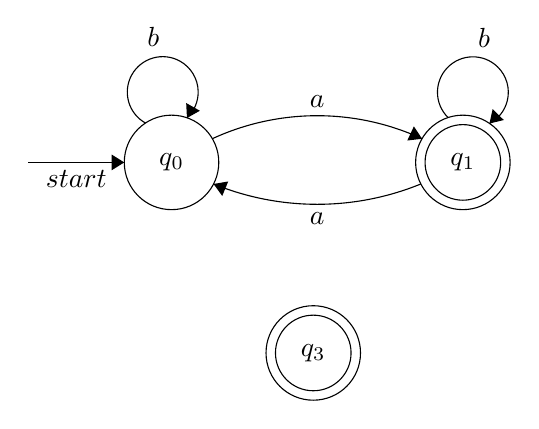
\begin{tikzpicture}[scale=0.2]
        \tikzstyle{every node}+=[inner sep=0pt]
        \draw [black] (16.1,-27) circle (3);
        \draw (16.1,-27) node {$q_0$};
        \draw [black] (34.6,-27) circle (3);
        \draw (34.6,-27) node {$q_1$};
        \draw [black] (34.6,-27) circle (2.4);
        \draw [black] (25.1,-39.1) circle (3);
        \draw (25.1,-39.1) node {$q_3$};
        \draw [black] (25.1,-39.1) circle (2.4);
        \draw [black] (7,-27) -- (13.1,-27);
        \fill [black] (13.1,-27) -- (12.3,-26.5) -- (12.3,-27.5);
        \draw (10.05,-27.5) node [below] {$start$};
        \draw [black] (18.69,-25.495) arc (114.75276:65.24724:15.906);
        \fill [black] (32.01,-25.5) -- (31.49,-24.71) -- (31.07,-25.61);
        \draw (25.35,-23.53) node [above] {$a$};
        \draw [black] (31.934,-28.368) arc (-67.77817:-112.22183:17.409);
        \fill [black] (18.77,-28.37) -- (19.32,-29.13) -- (19.7,-28.21);
        \draw (25.35,-30.16) node [below] {$a$};
        \draw [black] (14.455,-24.505) arc (241.12502:-46.87498:2.25);
        \draw (14.95,-19.7) node [above] {$b$};
        \fill [black] (17.08,-24.18) -- (17.9,-23.72) -- (17.03,-23.23);
        \draw [black] (33.67,-24.16) arc (225.8699:-62.1301:2.25);
        \draw (35.95,-19.71) node [above] {$b$};
        \fill [black] (36.29,-24.53) -- (37.2,-24.31) -- (36.49,-23.61);
    \end{tikzpicture}
\end{center}

Автоматы удобно представлять не набором множеств, а автоматом (Диаграмма Мура).

Каждое состояние обозначаем отдельным кругом (внутри впишем название состояния). Двойной кружок - принимающее состояние. Входная стрелка у начального состояние. Определим переходы: переход из состояния из $q_0$ в $q_1$ по символу a обозначим стрелкой. Впишем обратный переход. Петля будет вести из данного состояния в него же.

Автомат принимает слово с точки зрения графов - есть путь из начального состояния в принимающее, если автомат ДКА, то это путь определенном однозначно, для НКА не обязательно путь должен быть определен однозначно, и вдоль этого пути написано наше слово, принадлежность которого мы проверяем.

Распишем формально наш автомат.
\begin{enumerate}
    \item {\bfseries\itshape{Q}} - \{$q_0, q_1, q_3$\}
    \item $\boldsymbol{\Sigma}$ - \{$a,b$\};
    \item $\boldsymbol{q_0}$ -$q_0$
    \item $\boldsymbol{\delta}$ : $(\{q_0,b,q_0\}, \{q_0,a,q_1\},\{q_1,b,q_1\},\{q_1,a,q_0\})$
    \item $\boldsymbol{F} \subset \boldsymbol{Q}$ - \{$q_1,q_3$\}
\end{enumerate}

\textbf{Конфигурация автомата}
Конфигурацией конечного автомата называется $\mathcal{A} = \langle Q, \Sigma, q_s, F, \delta\rangle$ называется элемент множества $Conf(\mathcal{A}) = Q\times \Sigma^*$

\textbf{Отношение достижимости}
Зададим следующее отношение $\vdash^* \ \subset \ Conf(\mathcal{A})^2$:
\begin{itemize}
    \item $\forall q \in Q, w \in \Sigma^*: (q, w) \vdash^* (q, w)$
    \item $(q_1, xay) \vdash^* (q_2, ay) \vee (q_2, a, q_3) \in \delta \Rightarrow (q_1, xay) \vdash^* (q_3, y).$
\end{itemize}
Если $\forall x: (p, wx) \vdash^* (q, x)$, то будем писать $p \xrightarrow{w} q$.


\textbf{Слово принимаемое автоматом}
Будем говорить что слово $w$ принимается автоматом если для некоторого $q_f \in F$ верно $(q_s, w) \vdash^* (q_f, \varepsilon)$. Иначе говоря, если <<идя по стрелочкам>> в автомате по этому слову и правильно выбирая путь можно дойти до финального состояния.

\textbf{Язык принимаемый автоматом}
Язык автомата $\mathcal{A}$ --- это множество $L(\mathcal{A})$ всех слов принимаемых автоматом. Будем говорить, что конечный автомат принимает язык $B$ если $B = L(\mathcal{
        A})$. Будем говорить что два автомата $\mathcal{A}, \mathcal{B}$ эквивалентны, если $L(\mathcal{A})=L(\mathcal{B})$.

\textbf{Автоматный язык}
Язык называется автоматным если он принимается каким-либо конечным автоматом.

\textbf{Теорема Клини}
Класс автоматных языков и класс регулярных языков совпадают.

\begin{definition}{}{}
    $FollowPos(i \sigma)$ - {i $\sigma'$: i $\sigma'$ может идти в слове после $i\sigma$}
\end{definition}


Будем строить ДКА по следующему РВ с помощью вспомогательного множества --- $FollowPos$
\[
    R = \underset{0}{\rhd}(\underset{1}{a}\underset{2}{a}|\underset{3}{b})^{*}\underset{4}{b}(\underset{5}{a}|\underset{6}{b})^{*}\underset{7}{a}\underset{8}{\lhd}.
\]

Чтобы вычислить множество $FollowPos$, нам понадобится представление формулы в виде графа, который называется синтаксическим деревом:


\begin{figure}[h!tp]
    \centering
    \includegraphics[scale=0.5]{images/SintTree.PNG}
    \caption{Синтаксическое дерево}
    \label{fig:SyntaxTree1}
\end{figure}

Как же с помощью него вычислять функцию $FollowPos$? На самом деле одного синтаксического дерева недостаточно, нам придется ввести ещё три специальных атрибута. Пусть $u$ - узел синтаксического дерева, тогда:
\begin{definition}Символом $f_{u}$ будем обозначать значение атрибута $FirstPos(u)$ "--- множество номеров позиций, с которых может начинаться слово из $R_u$, где ($R_u$ - регулярное выражение, задаваемое вершиной $u$) \end{definition}

\begin{definition}
    Символом $l_{u}$ будем обозначать значение атрибута $LastPos(u)$ "--- множество номеров позиций, в которых может заканчиваться слово из $R_u$, где ($R_u$ - регулярное выражение, задаваемое вершиной $u$)
\end{definition}

\begin{definition}
    Атрибут $nullable(u)$ показывает содержит ли $R_u$ пустое слово ($T$ и $F$)
\end{definition}

Эти атрибуты вычисляются снизу вверх: зная атрибуты дочерних
узлов, вычисляются атрибуты родителя.
\begin{figure}[h!tp]
    \centering
    \includegraphics[scale=0.5]{images/7.PNG}
    \caption{Вычисление атрибутов для одного из узлов}
    \label{fig:SampleNode}
\end{figure}

В примере на рисунке $2$ левый узел имеет атрибут $nullable$ равный $True$, а значит конкатенация (корень данного поддерева) может начинаться как с $f_u$, так и с $f_v$. С другой стороны итоговая конкатенация может заканчиваться только с $f_v$, так как правый узел имеет атрибут $nullable$ равный $False$. Атрибут $nullable$ итоговой конкатенации тоже будет равен $False$, так как мы конкатенируем слова, одно из которых точно не может оказаться пустым.


После нескольких итераций вычислений таких атрибутов мы получаем готовое синтаксическое дерево:
\begin{figure}[h!t!p]
    \centering
    \includegraphics[scale=0.5]{images/FullSintTree.PNG}
    \caption{Готовое синтаксическое дерево}
    \label{fig:SyntaxTree2}
\end{figure}


Теперь, используя рисунок, мы можем найти необходимое множество $FollowPos$ по следующему алгоритму:
\begin{enumerate}
    \item Положим сначала $FollowPos(i) = \varnothing$ для каждого номера $i$
    \item Для каждой вершины-конкатенации $u\cdot v$, для каждого $i \in LastPos(u)$ добавим к $FollowPos(i)$ множество $FirstPos(v)$.
    \item Для каждой вершины-итерации $u^{*}$, для каждого $i \in LastPos(u)$ добавим к
          \\$FollowPos(i)$  множество $FirstPos(u)$.
\end{enumerate}

Построим таблицу множества $FirstPos$ для нашего регулярного выражения:
\begin{table}[h!]
    \centering
    \begin{tabular}{c|c}
        $i$   & $FollowPos(i)$ \\ \hline
        $1_a$ & $2_a$          \\
        $2_a$ & $1_a,3_b,4_b$  \\
        $3_b$ & $1_a,3_b,4_b$  \\
        $4_b$ & $5_a,6_b,7_a$  \\
        $5_a$ & $5_a,6_b,7_a$  \\
        $6_b$ & $5_a,6_b,7_a$  \\
        $7_a$ & $8_{\lhd}$
    \end{tabular}
    \caption{множество $FirstPos$}
\end{table}

Теперь с помощью таблицы с $FirsPos$ мы можем построить следующий ДКА:
\begin{figure}[ht!p]
    \centering
    \includegraphics[scale=0.5]{images/DKA.PNG}
    \caption{ДКА по таблице $FirstPos$}
    \label{fig:DFA}
\end{figure}

Начальное состояние автомата "--- это корень синтаксического дерева, поскольку атрибут $FirstPos(\text{Корень})$ как раз и будет указывать нам $FollowPos$ в самом начале. Далее проходим по таблице и строим итоговый автомат.


$\delta(S,b) = \bigcup followpos(\bigcup b)$

Проблема данного алгоритма в том, что если вы возьмете РВ и построите по нему ДКА, то оно окажется очень большим. Из-за экспоненциального роста возникают проблемы с памятью. Чтобы решить данную проблему зачастую используют НКА.

Алгоритм построения НКА мы рассмотрим на следующей лекции, а сейчас давайте построим НКА использую такой же  формализм, что и выше.

Начальное состояние - нулевая позиция. Из него будеь переход по $\varepsilon$ во все позиции, с которых слово может начинается.

Дальше для каждого отдельного символа и для каждой отдельной позиции будет просто переходы во все позиции по $followpos$. Мы уже знаем, что по символу $a$ идет переход в позицию $2a$. Из кружка, в котором написан символ позиции, идет переход во все кружки с $followpos$ от этой позиции и на переходе будет написан этот символ. Но всюду придется заменить маркер начала слова на пустое слово, и в конце добавляем новую вершину - маркер конца слова, и это состояние сделаем принимающим.

Еще раз алгоритм построения:
\begin{enumerate}
    \item Множество состояний это множество позиций
    \item Из позиции есть переход во все позиции из множества $followpos$ этот переход должен быть именно по символу из $followpos$
    \item Принимающее состояние единственное - маркер конца слова
    \item Все выходы из принимающего состояния - эпсилон переходы
\end{enumerate}


\begin{center}
    \begin{tikzpicture}[scale=0.2]
        \tikzstyle{every node}+=[inner sep=0pt]
        \draw [black] (21.1,-22.9) circle (3);
        \draw (21.1,-22.9) node {$\rhd$};
        \draw [black] (40.6,-14.5) circle (3);
        \draw (40.6,-14.5) node {$1_a$};
        \draw [black] (41.9,-26.2) circle (3);
        \draw (41.9,-26.2) node {$3_b$};
        \draw [black] (27.9,-35.9) circle (3);
        \draw (27.9,-35.9) node {$4_b$};
        \draw [black] (53.2,-14.5) circle (3);
        \draw (53.2,-14.5) node {$2_a$};
        \draw [black] (41.2,-36.6) circle (3);
        \draw (41.2,-36.6) node {$\lhd$};
        \draw [black] (41.2,-36.6) circle (2.4);

        \draw [black] (43.6,-14.5) -- (50.2,-14.5);
        \fill [black] (50.2,-14.5) -- (49.4,-14) -- (49.4,-15);
        \draw (46.9,-15) node [below] {$a$};
        \draw [black] (23.86,-21.71) -- (37.84,-15.69);
        \fill [black] (37.84,-15.69) -- (36.91,-15.54) -- (37.31,-16.46);
        \draw (31.84,-19.21) node [below] {$\varepsilon$};
        \draw [black] (24.06,-23.37) -- (38.94,-25.73);
        \fill [black] (38.94,-25.73) -- (38.23,-25.11) -- (38.07,-26.1);
        \draw (31.09,-25.15) node [below] {$\varepsilon$};
        \draw [black] (22.49,-25.56) -- (26.51,-33.24);
        \fill [black] (26.51,-33.24) -- (26.58,-32.3) -- (25.7,-32.76);
        \draw (23.82,-30.55) node [left] {$\varepsilon$};
        \draw [black] (30.9,-36.06) -- (38.2,-36.44);
        \fill [black] (38.2,-36.44) -- (37.43,-35.9) -- (37.38,-36.9);
        \draw (34.49,-36.81) node [below] {$b$};
        \draw [black] (9.9,-22.9) -- (18.1,-22.9);
        \fill [black] (18.1,-22.9) -- (17.3,-22.4) -- (17.3,-23.4);
        \draw (14,-23.4) node [below] {$start$};
    \end{tikzpicture}
\end{center}

Очевидно, регулярность будет сохраняться для любых композиций приведенных выше операций. Поэтому регулярным языком будет результат любой операции, которую можно, так сказать, "выразить в элементарных функциях". \\
Например, симметрическая разность двух регулярных языков:
\[X \triangle Y = (X \ \backslash \ Y) \cup (Y \ \backslash \ X) = (X \cup Y) \ \backslash \ (Y \cap X)\]
будет регулярным языком. \\
Разность двух регулярных языков также будет регулярна, так как
\[X \ \backslash \ Y = X \cap \overline{Y}\]

    \section{Контекстно-свободные грамматики. Автоматы с магазинной памятью. Эквивалентность
    автоматов с магазинной памятью и контекстно-свободных грамматик.}

    \section{Архитектура Фон-Неймана. Принципы однородности памяти, адресности и
    программного управления. Гарвардская архитектура, отличия от архитектуры Фон-
    Неймана. Примеры реализаций.}

    \section{Абстрактные структуры данных: списка, вектора, деревья поиска. Их асимптотики для
    операций поиска элемента и вставки новых элементов в середину или конец. Примеры
    реализаций.}

    \section{Целочисленная арифметика в представлении компьютера. Знаковые и беззнаковые
    значения, способы представления отрицательных значений. Целочисленное
    переполнение и его контроль. Длинная целочисленная арифметика.}
    \columnbreak

    \section{Вещественная арифметика. Представления с фиксированной и плавающей точкой.
    Стандарт IEEE754. Специальные вещественные значения, определенные стандартом
    IEEE754 и операции над ними.}

    \section{Устройство виртуального адресного пространства процесса. Стек и куча. Динамическая
    загрузка библиотек. Механизм трансляции адресов из виртуального в физическое
    адресное пространство.}
    \section{Операционные системы и их компоненты. Ядро операционных систем. Системные
    вызовы и их отличия от обычных библиотечных функций. Способы реализации
    системных вызовов (прерывания, sysenter, syscall).}
    \subsection*{Компоненты операционной системы}

      \begin{definition}{}{}
        \textit{Ядро} --- программа, которая запускается самой первой. Имеет привилегированное положение на процессоре и может взаимодействовать с <<железом>> напрямую.
      \end{definition}

      \begin{definition}{}{}
        \textit{Базовые библиотеки}: зачастую входят в состав операционной системы, потому что привязаны к определенному ядру (версии ядра), чтобы максимально использовать его функциональность. 
      \end{definition}

      \begin{definition}{}{}
      \textit{Служебные сервисы} --- ведение логов, обработка сетевых соединения, и т.д.
      \end{definition}

      \begin{definition}{}{}
      \textit{Минимальная пользовательская оболочка} --- чтобы пользователь мог взаимодействовать с системой.
      \end{definition}

      \subsection*{Процессы}

      \begin{definition}{}{}
      \textit{Процесс} --- любой экземпляр программы, работающей в операционной системе.
      \end{definition}

      Примеры:
      \begin{itemize}
        \item Приложения
        \item Фоновые сервисы (демоны)
        \item Команды в терминале
      \end{itemize}

      Главные команды для мониторинга процессов:
      \begin{itemize}
        \item ps -A -- список процессов
        \item pstree -- иерархия процессов
        \item top
      \end{itemize}

      \subsection*{UNIX программы}

      Программы:
      \begin{itemize}
        \item \textbf{Бинарные исполняемые файлы.}
        \item \textbf{Текстовый файл, начинающийся с \#!.} После \#! указывается путь к интерпретатору (например, \#!/bin/bash). Это могут быть скрипты на Python/Perl/Escript или Shell скрипт.
      \end{itemize}

      Название файла и его расширение не имеет значения. Любой файл, имеющий атрибут 
      <<исполняемый>> является программой.

      \subsection*{UNIX пользователи}

      Единственные привилегированный пользователь: root (UID = 0).

      Непривилегерованные пользователи:
      \begin{itemize}
        \item Реальные пользователи, которые могут войти в систему (UID $\ge$ 1000)
        \item Фейковые пользователи, привязанные к сервисам (UID $<$ 1000).
      \end{itemize}

      \textbf{Зачем сервисам нужны фейковые пользователи?}
      Допустим, у вас есть веб-сервер и сервер баз данных. Теоретически какой-то пользователь
      может подключиться к веб-серверу и найти там уязвимость. Для того, чтобы 
      минимизировать возможный ущерб от уязвимости в одном из процессов, процессы запускаются
      под разными пользователями и не имеют права общаться друг с другом.

      Непривилегерованные пользователи могут временно получить 
      дополнительные привилегии:

      \begin{itemize}
        \item su - запускает терминал от имени root
        \item sudo - запускает любую программу от имени root
        \item Запустить программу с атрибутом SUID и владельцем root. SUID атрибут означает, что при запуске программа
        исполняется от того пользователя, кто является владельцем файла. Кстати, так и 
        работает команда sudo, владелец sudo - root, а также у sudo проставлен атрибут SUID.
        \item Запустить программу с <<capabilities>> флагами. Эти флаги позволяют тонко настроить, что можно делать программе, а что - нельзя.
      \end{itemize}

      \subsection*{UNIX межпроцессорное взаимодействие}

      Процессы работают изолированно друг от друга. Единственный способ взаимодействовать друг с другом --- использовать методы межпроцессорного взаимодействия ядра (Inter-Process Communication, IPC):

      \begin{itemize}
        \item {Сигналы} для коротких сообщений
        \item {Каналы и сокеты} для последовательных данных
        \item {Разделяемая память}, в которой хранятся большие куски данных
      \end{itemize}

      \subsection*{Процесс запуска}

      \begin{enumerate}
        \item {Загрузчик} с диска или UEFI материнской платы выполняется в привилегированном режиме
        \item Загрузчик запускает {ядро}, тоже в привилегированном режиме.
        \item Ядро запускает первый непривелигерованный процесс: {init или systemd}.
      \end{enumerate}

      \subsection*{Сервисы (``Демоны'')}
      \begin{definition}{}{}
        \textit{Сервисы} --- это специальные системные службы, которые работают в фоновом режиме.
      \end{definition}

      Минимальный сет во многих системах:

      \begin{itemize}
        \item \textbf{dhclient} -- держит активным полученный IP адрес в сети
        \item \textbf{getty} -- переключение между графическим/консольным входом в систему
        \item \textbf{sshd} -- подключение по ssh
        \item \textbf{ntpd или chronyd} -- синхронизация времени
        \item \textbf{syslogd} -- системный лог
      \end{itemize}

      \subsection*{\#!/bin/sh}

      В терминале вы работаете в интерпретаторе \texttt{shell}. \texttt{shell} предоставляет возможность выполнять
      команды и последовательности команд.

      Бывают разные интерпретаторы \texttt{shell}:
      \begin{itemize}
        \item самодостаточный \texttt{shell} program: \textbf{FreeBSD}
        \item основной в \texttt{Linux}: \textbf{bash}
        \item debian: \textbf{dash}
        \item alpine: \textbf{busybox}
        \item maxOS X: \textbf{zsh}
      \end{itemize}

      \subsection*{Системный демон (systemd)}
      \begin{definition}{}{}
      Процесс, который управляет всеми остальными процессами. При этом сам является обычным процессом. \texttt{Systemd} пришел на замену INIT-процессу.

      \end{definition}

      Чем systemd лучше?
      \begin{itemize}
        \item Устранение интерпретации \texttt{shell} скриптов. 
        \item Запуск сервисов параллельно
      \end{itemize}

      \subsubsection*{Концепты systemd}

      \begin{itemize}
        \item Сервисы
        \item Цели:
          \begin{itemize}
            \item \textit{Стандартные цели}. Например, уровни \texttt{init} в System-V:
              \begin{itemize}
                \item poweroff.target (init 0)
                \item rescue.target (init 1)
                \item multi-user.target (init 3)
                \item graphical.target (init 5)
                \item reboot.target (init 6)
                \item sleep.target и hibertate.target (не присутствуют в System-V)
              \end{itemize}
            \item \textit{Специальные цели}
          \end{itemize}
      \end{itemize}

      \subsection*{Фоновые задачи}

      \begin{itemize}
        \item \textbf{Нет привязанного к задаче терминала.} Для того, чтобы сигнал \texttt{SIGHUP}
        не останавливал исполнение задачи используется команда \texttt{nohup}.
        \item \textbf{Пишут в лог.} Иногда пишут данные в какую-то старинную 
        локальную почтовую систему.
        \item \textbf{Запускается в единственном экземпляре.} Обычно это достигается
        с помощью file lock.
      \end{itemize}

      \subsection*{Дистрибутивы \texttt{Linux}}

      Ядро называется Linux. Базовая система --- минимальная юзабельная система.

      \textit{Дистрибутив}:
      \begin{itemize}
        \item Ядро
        \item Базовая система
        \item GUI оболочка
        \item Программное обеспечение 
      \end{itemize}

      \subsubsection*{Какие есть дистрибутивы?} 

      Общего назначения:
      \begin{itemize}
        \item OpenSUSE
        \item Fedora
        \item Debian
        \item Ubuntu
      \end{itemize}

      Специфические дистрибутивы:
      \begin{itemize}
        \item Alpine Linux --- очень легковесный, поэтому его
        хорошо ставить на виртуальную машину.
        \item Kali Linux --- используется для тестов на безопасность.
      \end{itemize}
      \begin{definition}{}{}
        \underline{Прерывание} --- это сигнал от программного или аппаратного обеспечения,
        сообщающий процессору о наступлении какого-либо события, требующего немедленного внимания.
      \end{definition}
      
      \subsection*{Обработка прерывания в x86}
      
      \begin{itemize}
        \item Каждое устройство имеет свой собственный номер прерывания (IRQ).
        \item Процессор получает сигнал INT и прекращает исполнение текущекого контекста.
        \item Каждое прерывание имеет свой адрес в векторе прерываний.
        \item Прерывания бывают не только аппаратные. Его можно сымитировать, 
        вызвав прерывание программно.
      \end{itemize}
      
      \subsection*{Маска прерывания}
      
      Иногда хочется запретить прерывания в каком-то месте. Для этого существует маска прерываний.
      
      \subsection*{Номера прерываний}
      
      \begin{itemize}
        \item 0 --- нажатие на кнопку включения или Reset
        \item 1...15 --- Аппаратные прерывания. Тут задействованы реальные железяки.
        \item 16+ --- программные прерывания, вызванные через int.
      \end{itemize}
      
      \subsection*{Базовый вектор прерываний}
      
      Кто прописывает нам функции, которые будут вызваны при прерывании?
      \begin{itemize}
        \item BIOS --- содержит весь минимальный набор функций, нужный после включения.
        \item Обработка железяк (клавиатура, ...).
        \item Функции для обращения к данным на диске и загрузки операционной системы.
      \end{itemize}
      
      \subsection*{Обработка прерываний}
      
      \begin{itemize}
        \item Сохранить EIF на стек
        \item Проставить 1 в флаг IF
        \item Перейти на инструкцию по адресу IDTR + offset
      \end{itemize}
      
      \underline{Перед вызовом обработчика прерывания:}
      \begin{itemize}
        \item Сбросить флаги
        \item Переключить текущее адресное пространство
        \item Заменяется стек
      \end{itemize}
      
      \underline{Выполнение функции обработчика прерывания:}
      \begin{itemize}
        \item Сохранить текущее значение регистров и флагов
        \item что-то поделать...
        \item бернуть состояние регистров и флагов обратно
      \end{itemize}
      
      \subsection*{Ядро}
      
      При запуске операционной системы есть одна программа - ядро. Она может делать все что угодно.
      
      \subsection*{Режимы исполнения (x86)}
      
      \textbf{Обычный режим:}
      \begin{itemize}
        \item Процесс имеет доступ только к своей собственной памяти.
        \item Виртуальное адресное пространство каждого процесса начинается с адреса 0.
        \item Процесс не может взаимодействовать с устройствами.
      \end{itemize}
      
      \textbf{Превилегированный режим:}
      \begin{itemize}
        \item Полный доступ к физической (не виртуальной) памяти.
        \item Полный доступ к портам ввода/вывода.
        \item Некоторые дополнительные команды, не доступные в обычном режиме исполнения.
      \end{itemize}
      
      \begin{definition}{}{}
        \underline{Системный вызов} --- механизм для взаимодействия обычных процессов с ядром. 
        Он позволяет обратиться к функциональности ядра, чтобы сделать недоступные в обычном
        режиме операции.
      \end{definition}
      
      \subsection*{Ядро}
      
      \begin{itemize}
        \item Обычный ELF файл.
        \item Запускается в привилегированном режиме.
        \item Отвечает за взаимодействие с железом.
      \end{itemize}
      
      \subsection*{Запуск ядра}
      
      \begin{itemize}
        \item Проинициализировать устройства.
        \item Проинициализировать вектор прерываний.
        \item Найти, загрузить и запустить все драйвера.
        \item Понизить привилегии процессора.
        \item Запустить первый пользовательский процесс --- init.
      \end{itemize}
      
      \subsection*{Взаимодействие с ядром (x86)}
      
      \begin{itemize}
        \item Все процессы непривилегированы.
        \item Единственный способ получить доступ к железу --- переключиться в 
        режим ядра.
        \item Все прерывания переключают процессор в привилегированный режим.
        \item Используйте int для того, чтобы получить доступ к системным вызовам.
      \end{itemize}
      
      \subsection*{Типы архитектуры ядер}
      
      \begin{itemize}
        \item \textbf{Монолитные ядра.} Одна большая программа, которая исполняется 
        в привилегированном режиме. Примеры: Linux.
        \item \textbf{Микроядерная.} Только небольшая часть ядра запускается в привилегированном
        режиме. Большая часть подсистем работает как пользовательские процессы. Примеры: Minix3.
        \item \textbf{Гибридная.} Модульная, но не одна большая программа, запускаемая в
        привилегированном режиме. Примеры: Windows, Mac, BSD или Linux.
      \end{itemize}
      
      \subsection*{Системные вызовы}
      
      Системный вызов можно осуществить с помощью:
      \begin{itemize}
        \item int 0x80 (Linux, BSD)
        \item sysenter/sysleave инструкции (Intel)
        \item syscall/sysret инструкции (AMD64/x86\_64)
      \end{itemize}
      
      \subsection*{INT 0x80}
      
      \begin{itemize}
        \item В eax сохраняется номер системного вызова
        \item Параметры сохраняются в ebx, ecx, ...
        \item Возвращаемое значение сохраняется в eax
        \item Конвенции вызовов отличаются от принятых в языке C!
      \end{itemize}
      
    \section{Процессы и потоки. Сходства и различия между ними. Реализация многозадачности и
    алгоритмы планирование задач в операционных системах.}
    \subsection*{Что такое процесс?}

    \begin{definition}{}{}
      \underline{Процесс} --- это экземпляр программы в одном из состояний выполнения. Каждый
      из процессов выполняется в своем изолированном адресном пространстве.
    \end{definition}
    
    \subsection*{Аттрибуты процесса}
    
    Память:
    \begin{itemize}
      \item Значения регистров процессора.
      \item Таблицы и каталоги страниц виртуального адресного пространства.
      \item Private и Shared страницы памяти.
      \item Отображение файлов в память.
      \item Отдельный стек в ядре для обработки системных вызовов.
    \end{itemize}
    
    Файловая система:
    \begin{itemize}
      \item Таблица файловых дескрипторов.
      \item Текущий каталог.
      \item Корневой каталог.
      \item Маска аттрибутов создания нового файла umask. 
    \end{itemize}
    
    Другие аттрибуты:
    \begin{itemize}
      \item Переменные окружения
      \item Лимиты
      \item Счетчики ресурсов
      \item Идентификаторы пользователя и группы
    \end{itemize}
    
    \subsection*{Информация о процессах}
    
    Команда \textbf{ps} показывает список процессов, \textbf{top} --- потребление ресурсов.
    
    \subsection*{Жизненный цикл процессов}
    
    \begin{itemize}
      \item Выполняется (Running)
      \item Остановлен (Stopped)
      \item Временно приостановлен
        \begin{itemize}
          \item Suspended --- может быть завершен
          \item Disk Suspended --- не может быть завершен
        \end{itemize}
      \item Исследуется (Tracing)
      \item Зомби (Zombie)
    \end{itemize}
    
    \textbf{Как устроен планировщик заданий?}
    
    \subsection*{Round Robin}
    \textit{Windows 9x, старые UNIX}
    
    Аппаратный таймер время от времени генерирует прерывание, после чего планировщик
    выбирает, какой процесс будет выполняться дальше.
    
    \subsection*{Приоритет}
    
    \begin{definition}{}{}
      \underline{Приоритет процесс} --- это численное значение от -20 до 19. 
      Оно обозначает то, сколько раз пропустить планировщиком заданий.
    \end{definition}
    
    \begin{itemize}
      \item Значение от 
      \item Численное значение --- 
    \end{itemize}
    
    \subsection*{Многоуровневая очередь}
    \textit{Linux, xBSD, Mac, Windows}
    
    Эта схема отталкивается от того, что есть два типа процессов:
    \begin{itemize}
      \item Не очень активно взаимодействующие с внешним миром (что-то вычисляют). 
      Им надо просто не мешать выполняться. 
      \item Много взаимодействующие с пользователем. Их надо переключать быстро.
    \end{itemize}
    
    Есть набор очередей, уровней, которые рассположены по увеличению времени переключения.
    При переключении очереди, если процесс освободил процессор до следующего события, он
    перемещается в следующую очередь (более редко переключаемую), иначе --- в предыдущую.
    
    \subsection*{Ничегонеделание}
    
    while (1) {
      // Так делать очень плохо, потому что вы загружаете процессор
    }
    
    while (1) {
      sched\_yield(); // Передаем управление другому процессу
    }
    
    \subsection*{Создание процесса}
    
    Системный вызов fork().

    \subsection*{Копия процесса}
    
    При fork создается полная копия процесса. Память, регистры, ... --- точная копия.
    
    Не копируются:
    \begin{itemize}
      \item eax, rax
      \item Сигналы, ожидающие доставки
      \item Таймеры
      \item Блокировки файлов
    \end{itemize}
    
    \textbf{В связи с копированием всего адресного пространства может возникать необычное поведение.} Например, 
    буфер ввода и вывода тоже копируется. Поэтому если не сделать fflush, один и тот
    же текст может продублироваться.
    
    \subsection*{Ограничения}
    
    /proc/sys/kernel/pid\_max --- максимальное число одновременно запущенных процессов.
    /proc/sys/kernel/threads\_max --- максимальное число одновременно 
    выполняющихся потоков (каждый процесс --- уже один поток).
    
    \subsection*{Дерево процессов}
    
    \begin{itemize}
      \item Процесс с номером 1 --- systemd
      \item У каждого процесса кроме systemd есть свой родитель
      \item Если родитель процесса умирает, то его родителем становится systemd.
      \item Если ребенок умирает, про это узнает его родитель. 
    \end{itemize}
    
    \subsection*{Завершение работы процесса}
    
    \begin{itemize}
      \item Системный вызов \_exit(int)
      \item Функция exit(int)
      \item Оператор return в main
    \end{itemize}
    
    \subsection*{Ожидание завершения процесса}
    
    Системный вызов waitpid.
    
    \subsection*{Zombie процессы}
    
    Удалением зомби из таблицы процессов занимается родитель --- 
    вызовом wait или waitpid.
    
    \subsection*{exec}
    
    Системный вызом exec позволяет заместить тело процесса другой программой.
    
    \subsection*{Аттрибуты процесса, сохраняемые exec}
    
    \begin{itemize}
      \item Открытые файловые дескрипторы 
      \item Текущий каталог
      \item Лимиты процесса
      \item UID, GID
      \item Корневой каталог --- root.
    \end{itemize}
    \section{Проблема многопоточной синхронизации. Атомарные переменные и объекты
    блокировки. Неблокирующие структуры данных и их реализация.}
    \section{Интерконнект в вычислительном кластере. Отличие интерконнекта от глобальных
    компьютерных сетей. Основные характеристики интерконнекта. Топологии соединений
    узлов в вычислительном кластере, характеристики топологий.}
    \columnbreak

    \section{Понятие ускорения и масштабируемости параллельных программ. Закон Амдала.
    Оценка эффективности параллельных программ. Ярусно-параллельная форма
    программы.}

    \section{Параллельные и распределённые вычислительные системы. Парадигма Map-Reduce.
    Примеры, отличия. Распределенные файловые системы. Особенности хранения файлов
    в них. Репликация.
    }
\end{multicols}
\chapter{Основы анализа данных}

\AddToShipoutPictureBG*{%
  \AtPageUpperLeft{%
    \hspace{\paperwidth}%
    \raisebox{-\baselineskip}{%
      \makebox[-10pt][r]{\textbf{ТИИ}}
}}}%

\begin{multicols}{2}
    \raggedcolumns
    \section{Основные понятия машинного обучения. Основные постановки задач. Примеры
    прикладных задач.}

    \section{Линейные пространства. Векторы и матрицы. Линейная независимость. Обратная
    матрица.}

    \section{Производная и градиент функции. Градиентный спуск. Выпуклые функции.}

    \section{Случайные величины. Дискретные и непрерывные распределения. Примеры.}

    \section{Оценивание параметров распределений, метод максимального правдоподобия.
    Бутстрэппинг.}

    \section{Линейные методы классификации и регрессии: функционалы качества, методы
    настройки, особенности применения.}

    \section{Метрики качества алгоритм регрессии и классификации.}

    \section{Оценивание качества алгоритмов. Отложенная выборка, ее недостатки. Оценка полного
    скользящего контроля. Кросс-валидация. Leave-one-out.}

    \section{Деревья решений. Методы построения деревьев. Их регуляризация.}

    \section{Композиции алгоритмов. Разложение ошибки на смещение и разброс.}
    \columnbreak
    \section{Случайный лес, его особенности. Методы поиска выбросов в данных. Методы
    восстановления пропусков в данных. Работа с несбалансированными выборками.}

    \section{Нейронные сети: перцептрон, многослойный перцептрон. Автоэнкодеры и
    рекуррентные нейронные сети.}

    \section{Задача кластеризации. Алгоритм K-Means. Оценки качества кластеризации.
    Литература
    }
\end{multicols}
\chapter{Теория управления и\\[-20pt] \hfill эксперные системы}

\AddToShipoutPictureBG*{%
  \AtPageUpperLeft{%
    \hspace{\paperwidth}%
    \raisebox{-\baselineskip}{%
      \makebox[-10pt][r]{\textbf{ТИИ}}
}}}%

\begin{multicols}{2}
    \raggedcolumns
    \section{Собственные числа и собственные векторы матриц.}
    \section{Квадратичные формы. Свойства положительно полуопределенных и положительно
    определенных матриц.}
    \section{Теорема о существовании и единственности решения задачи Коши для системы
    обыкновенных дифференциальных уравнений.}
    \section{Устойчивость по Ляпунову динамических систем.}
    \section{Логика исчисления предикатов первого порядка. Дайте определения понятиям терм,
    предикат, формула. Перечислите основные отличия логики предикатов от логики
    высказываний. Синтаксис и семантика языка первого порядка. Примеры.}
    \section{Преобразование Фурье. Понятие о прямом и обратном преобразовании Фурье. Свойства
    преобразования Фурье.}
    \section{Вейвлет-преобразование и анализ временных рядов. Непрерывное, дискретное и
    быстрое вейвлет-преобразования. Основные понятия теории принятия решений, задача
    принятия решения, процесс принятия решения. Способы оценки, сравнения и выбора
    варианта. Описание подходов к решению задач коллективного выбора.}
    \columnbreak
    \section{Математические методы в экспертных системах. Основные компоненты экспертных
    систем. Этапы разработки. Инструменты разработки. Инженерия знаний.}
\end{multicols}
\end{document}
